% Options for packages loaded elsewhere
\PassOptionsToPackage{unicode}{hyperref}
\PassOptionsToPackage{hyphens}{url}
%
\documentclass[
]{book}
\usepackage{amsmath,amssymb}
\usepackage{lmodern}
\usepackage{iftex}
\ifPDFTeX
  \usepackage[T1]{fontenc}
  \usepackage[utf8]{inputenc}
  \usepackage{textcomp} % provide euro and other symbols
\else % if luatex or xetex
  \usepackage{unicode-math}
  \defaultfontfeatures{Scale=MatchLowercase}
  \defaultfontfeatures[\rmfamily]{Ligatures=TeX,Scale=1}
\fi
% Use upquote if available, for straight quotes in verbatim environments
\IfFileExists{upquote.sty}{\usepackage{upquote}}{}
\IfFileExists{microtype.sty}{% use microtype if available
  \usepackage[]{microtype}
  \UseMicrotypeSet[protrusion]{basicmath} % disable protrusion for tt fonts
}{}
\makeatletter
\@ifundefined{KOMAClassName}{% if non-KOMA class
  \IfFileExists{parskip.sty}{%
    \usepackage{parskip}
  }{% else
    \setlength{\parindent}{0pt}
    \setlength{\parskip}{6pt plus 2pt minus 1pt}}
}{% if KOMA class
  \KOMAoptions{parskip=half}}
\makeatother
\usepackage{xcolor}
\IfFileExists{xurl.sty}{\usepackage{xurl}}{} % add URL line breaks if available
\IfFileExists{bookmark.sty}{\usepackage{bookmark}}{\usepackage{hyperref}}
\hypersetup{
  pdftitle={Aplicación para el costeo de intervenciones de conservación marina},
  pdfauthor={Juan Carlos Villaseñor-Derbez},
  hidelinks,
  pdfcreator={LaTeX via pandoc}}
\urlstyle{same} % disable monospaced font for URLs
\usepackage{longtable,booktabs,array}
\usepackage{calc} % for calculating minipage widths
% Correct order of tables after \paragraph or \subparagraph
\usepackage{etoolbox}
\makeatletter
\patchcmd\longtable{\par}{\if@noskipsec\mbox{}\fi\par}{}{}
\makeatother
% Allow footnotes in longtable head/foot
\IfFileExists{footnotehyper.sty}{\usepackage{footnotehyper}}{\usepackage{footnote}}
\makesavenoteenv{longtable}
\usepackage{graphicx}
\makeatletter
\def\maxwidth{\ifdim\Gin@nat@width>\linewidth\linewidth\else\Gin@nat@width\fi}
\def\maxheight{\ifdim\Gin@nat@height>\textheight\textheight\else\Gin@nat@height\fi}
\makeatother
% Scale images if necessary, so that they will not overflow the page
% margins by default, and it is still possible to overwrite the defaults
% using explicit options in \includegraphics[width, height, ...]{}
\setkeys{Gin}{width=\maxwidth,height=\maxheight,keepaspectratio}
% Set default figure placement to htbp
\makeatletter
\def\fps@figure{htbp}
\makeatother
\setlength{\emergencystretch}{3em} % prevent overfull lines
\providecommand{\tightlist}{%
  \setlength{\itemsep}{0pt}\setlength{\parskip}{0pt}}
\setcounter{secnumdepth}{5}
\usepackage{booktabs}
\usepackage{amsthm}
\usepackage[spanish]{babel}
\makeatletter
\def\thm@space@setup{%
  \thm@preskip=8pt plus 2pt minus 4pt
  \thm@postskip=\thm@preskip
}
\makeatother
\ifLuaTeX
  \usepackage{selnolig}  % disable illegal ligatures
\fi
\usepackage[]{natbib}
\bibliographystyle{apalike}

\title{Aplicación para el costeo de intervenciones de conservación marina}
\usepackage{etoolbox}
\makeatletter
\providecommand{\subtitle}[1]{% add subtitle to \maketitle
  \apptocmd{\@title}{\par {\large #1 \par}}{}{}
}
\makeatother
\subtitle{Manual de usuario}
\author{Juan Carlos Villaseñor-Derbez}
\date{Última actualzación: Julio 25, 2022}

\begin{document}
\maketitle

{
\setcounter{tocdepth}{1}
\tableofcontents
}
\hypertarget{bienvenida}{%
\chapter{Bienvenida}\label{bienvenida}}

\hypertarget{sobre-la-aplicaciuxf3n}{%
\section{Sobre la aplicación}\label{sobre-la-aplicaciuxf3n}}

La aplicación de costeo de intervenciones de conservación marina te permite diseñar y costear una intervención. La intervención puede ser en forma de reservas marinas o proyectos de mejoramiento pesquero. La aplicación está disponible en \href{https://innovacionazul.shinyapps.io/AppCosteo/}{este link}.

\hypertarget{sobre-el-manual}{%
\section{Sobre el manual}\label{sobre-el-manual}}

El manual está disponible en tres formatos: página web, documento de PDF, o E-pub para kindle o similares. En la ágina web, la barra lateral te permite navegar entre capítulos y secciones. El capítulo \ref{intro} presenta una breve descripción de la jararquia de un presupusto y la interfaz de usuario. El capítulo \ref{llenado} muestra dos ejemplos de llenado de datos par aun presupuesto de REMA y un presupuesto de FIP. El capítulo \ref{explorar} describe el área de exploración y visualización de datos, así como la opción de dividir el presupuesto entre diferentes actores. El capítulo \ref{guardar} te muestra como guardar tu progreso, mientras que el capítulo \ref{cargar} te muestra como continuar un presupuesto anterior. Finalmente, el capítulo \ref{compartir} te muestra cómo compartir un presupuesto.

\hypertarget{contacto-a-desarrolladores}{%
\section{Contacto a desarrolladores}\label{contacto-a-desarrolladores}}

Para cualquier pregunta o comentario sobre este producto escribe al correo \href{mailto:rema@cobi.org.mx}{\nolinkurl{rema@cobi.org.mx}}. Tus observaciones nos ayudarán a mejorar nuestras herramientas.

\hypertarget{intro}{%
\chapter{Introducción}\label{intro}}

El número de iniciativas para establecer redes de Reservas Marinas (REMA) y Proyectos de Mejora Pesquera (FIP) está en aumento, y la gran mayoría de los esfuerzos se realizan con fondos filantrópicos. Sin embargo, al iniciar cualquier intervención, es común que los costos proyectados al futuro no estén claramente definidos. Esto puede afectar la sustentabilidad de la intervención al largo plazo.

Esta aplicación ayuda a estimar los costos aproximados necesarios para llevar a cabo dos tipos de intervenciones: establecer una reserva marina utilizado el modelo COBI, o un proyecto de mejoramiento pesquero. Su objetivo es ayudar a comunidades, organizaciones de la sociedad civil y tomadores de decisiones de planear sus inversiones con mayor claridad y transparencia.

\hypertarget{estructura}{%
\section{Estructura de un presupuesto}\label{estructura}}

La aplicación te permite generar un presupuesto jerárquico, definido de la siguiente manera:

\begin{itemize}
\item
  \textbf{Secciones}: Hay dos, una para Reservas Marinas (REMA) y una para Proyctos de Mejoramiento Pesquero (FIPS).
\item
  \textbf{Fases}: Las intervenciones se dividen en tres fases: Diseño, Implementación y Seguimiento.
\item
  \textbf{Subfase}: El número de subfases varía según el tipo de intervención y la fase, pero nos ayudan a categorizar los costos de manera más específica. La siguiente sección proporciona más detalles al respecto.
\item
  \textbf{Actividad}: Cada subfase se compone de diferentes actividades. Por ejemplo, la subfase de Socialización para el Diseño de una reserva marina tiene únicamente una actividad: Reuniones para presentar información de ZRP. Por otro lado, la subfase de identificación y socialización en la fase de diseño de FIPs tiene cuatro actividades.
\item
  \textbf{Elemento}: Para llevar a cabo cada actividad, es necesar con ciertos elementos. Es aquí donde pudes combinar precios y cantidades para determinar los costos de la actividad.
\end{itemize}

Por lo tanto, las secciones se dividen en fases. Las fases se dividen en subfases. Las subfases se dividen en actividades. Y las actividades se dividen en elementos.

\hypertarget{interfaz-de-usuario}{%
\section{Interfaz de Usuario}\label{interfaz-de-usuario}}

\hypertarget{barra-lateral}{%
\subsection{Barra lateral}\label{barra-lateral}}

La interfaz de usuario está diseñada para reflejar las estructura del presupuesto. Al entrar a la aplicación, lo primero que verás es una pantalla (Fig. \ref{fig:landing-page}). El lado izquierdo muestra el panel de control y navgación. El panel te permite navegar a través de las diferentes secciones de la aplicación. La sección predeterminada es la sección de ``Inicio'', donde se encuentra un pequeño resumen de la aplicación, así como enlances a este manual. También están disponibles las dos secciones que identifican el tipo de intervención (``Costeo de Reservas'' y ``Costeo de FIP''), y la sección para visualizar el presupuesto (``Gráficos''). Finalmente, observarás la zona de herramientas disponibles, como cargar un presupuesto anterior, descargar el presupuesto de la sesión, o compartir el estado de tu sesión con alguien más.

\begin{figure}
\centering
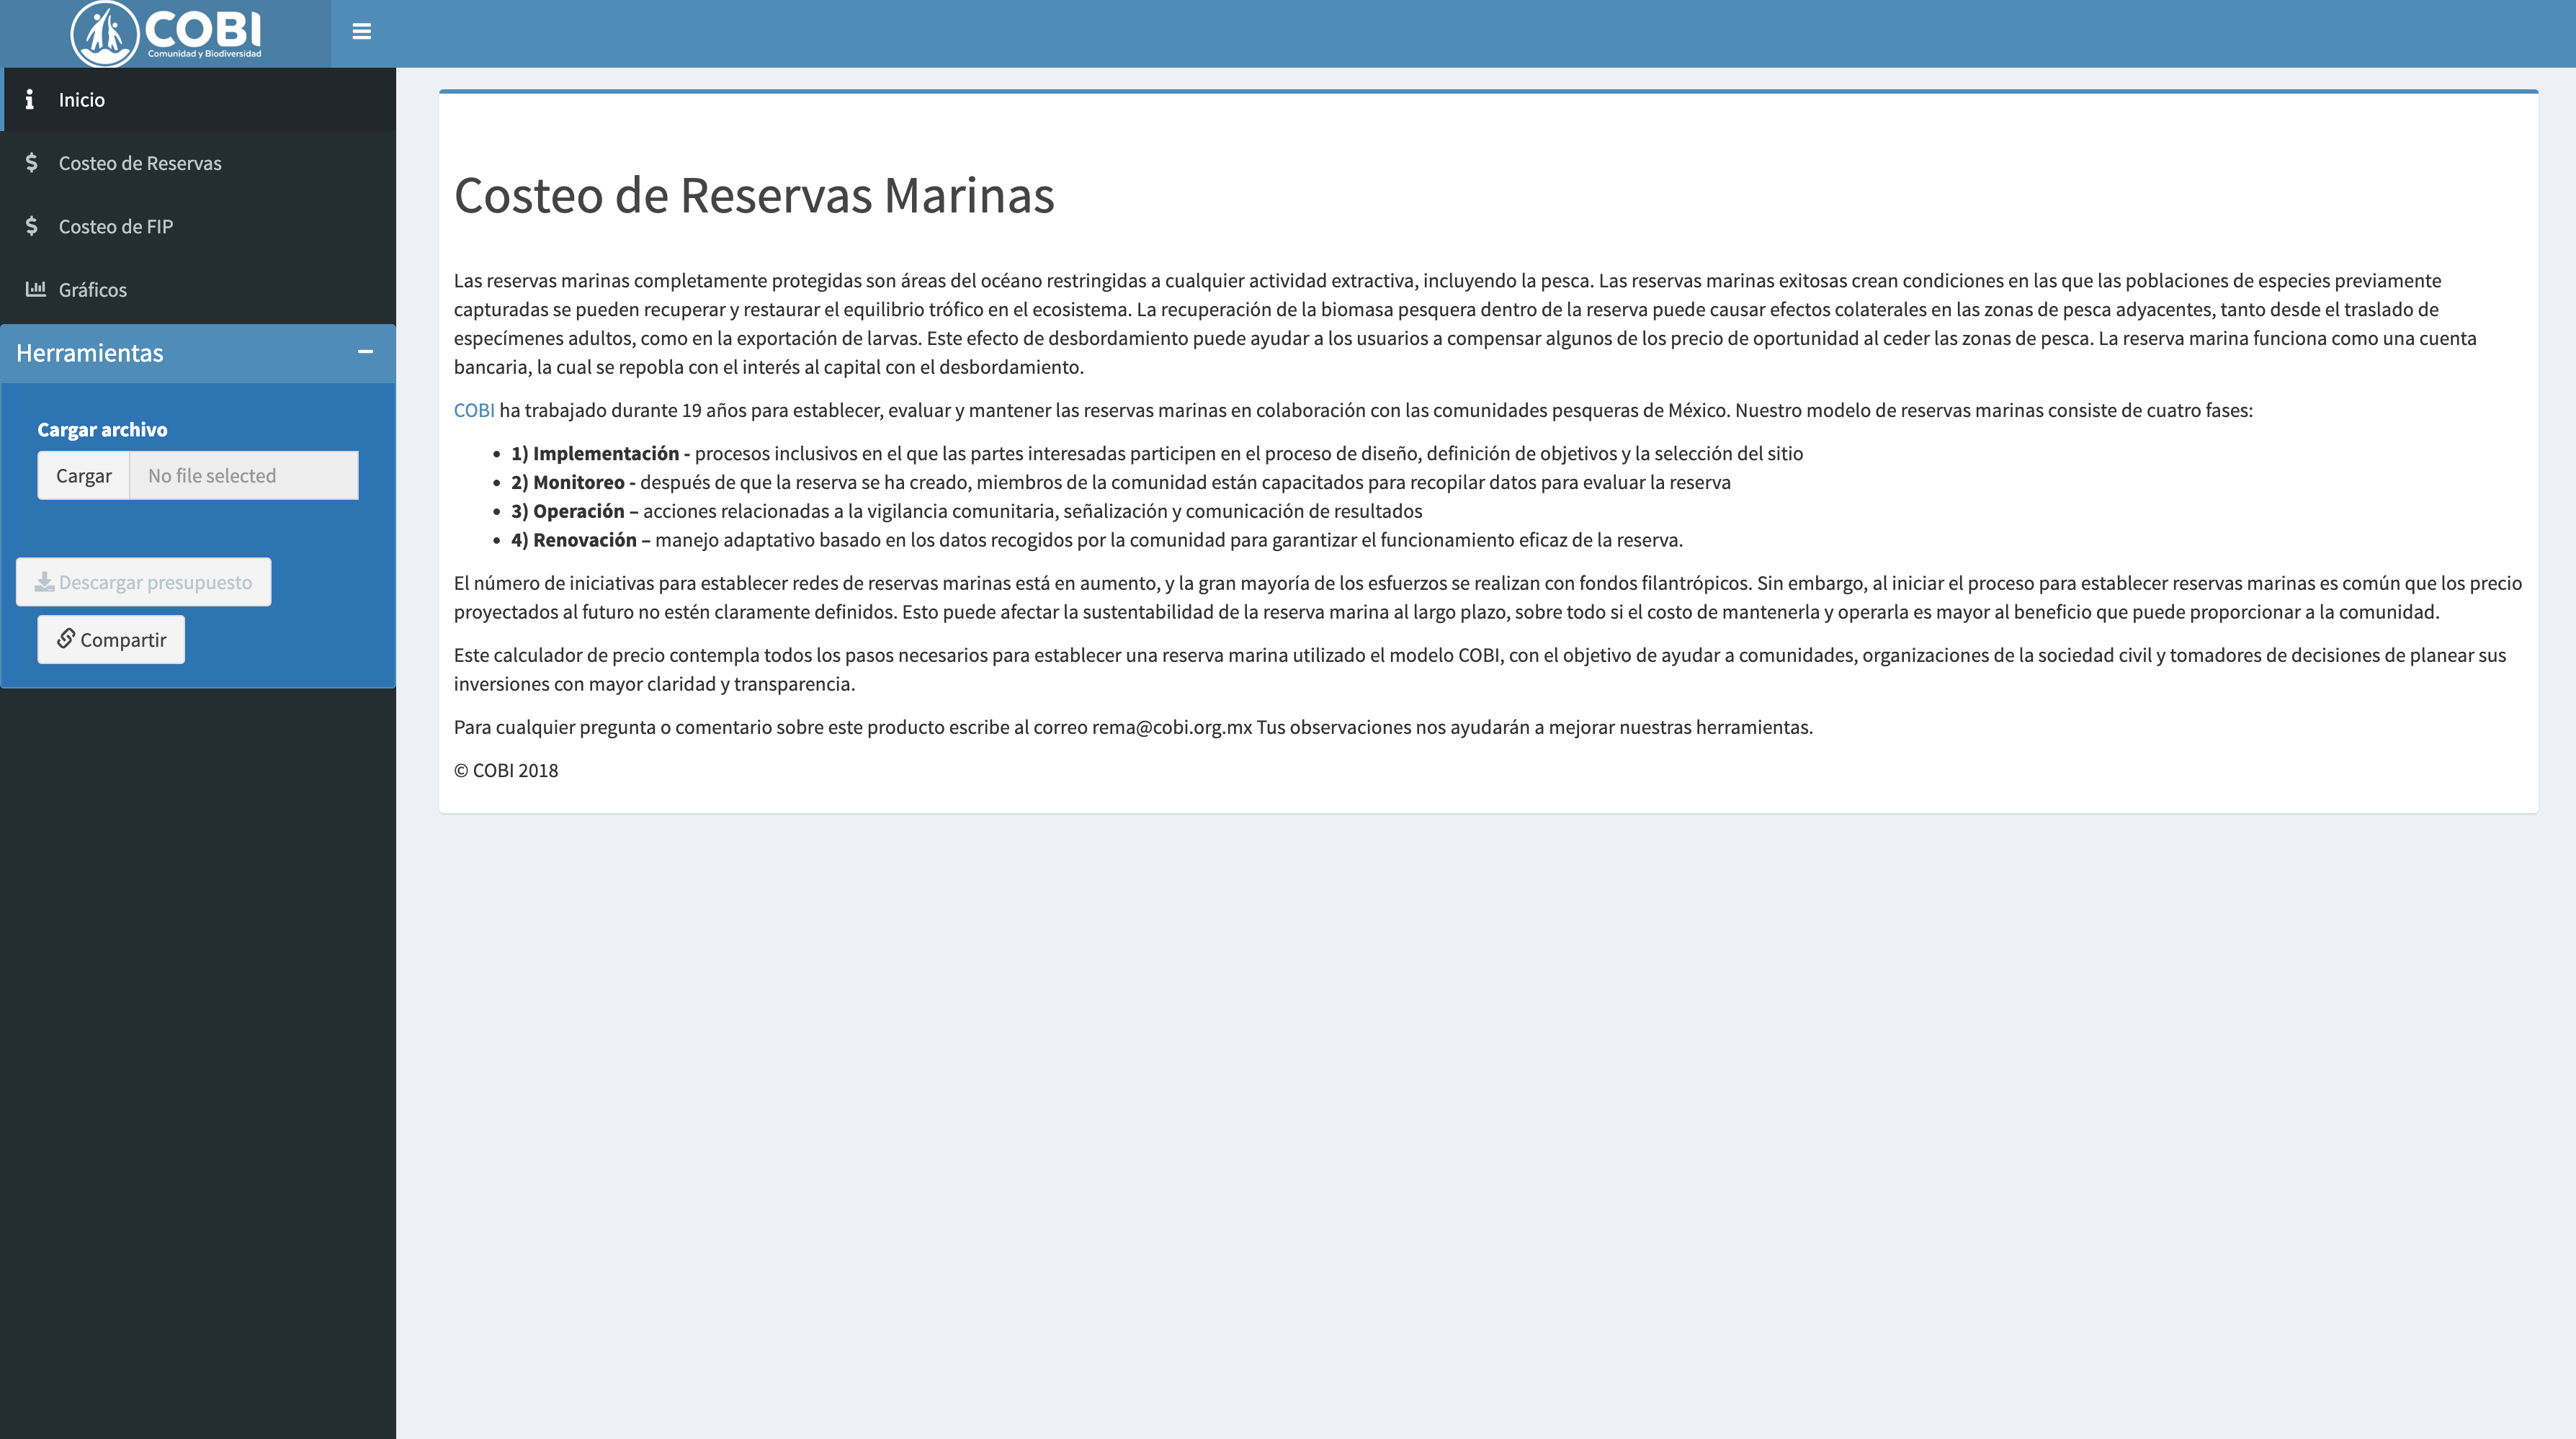
\includegraphics{images/Screen Shot 2022-07-25 at 2.43.50 PM.png}
\caption{\label{fig:landing-page}Página de bienvenida en la aplicación web.}
\end{figure}

\hypertarget{uxe1rea-de-trabajo}{%
\subsection{Área de trabajo}\label{uxe1rea-de-trabajo}}

Del lado derecho observarás el área de trabajo principal. Si estás trabajando en el llenado de un presupuesto, esta sección te mostrará los diferentes campos para que puedas ingresar los valores o explorar el presupuesto. Exploremos más a detalle cada una de estas.

La figura \ref{fig:filling-page} muestra el estado de la aplicación cuando el usuario ha seleccionado ``Costeo de Reservas'' en el menú lateral. En la zona superior del área de trabajo principal podrás observar tres pestañas con los nombres de ``Diseño'', ``Implementación'', y ``Seguimiento'', stas son las tres fases descritas en sección \ref{estructura}. La pestaña ``Implementación'' está seleccionada, indicado por la barra azul sobre su nombre. En este punto, la aplicación te muestra una ventana titulada ``Duración de la fase'' en la que especificaremos la duración del a fase de diseño de las reservas marinas.

\begin{figure}
\centering
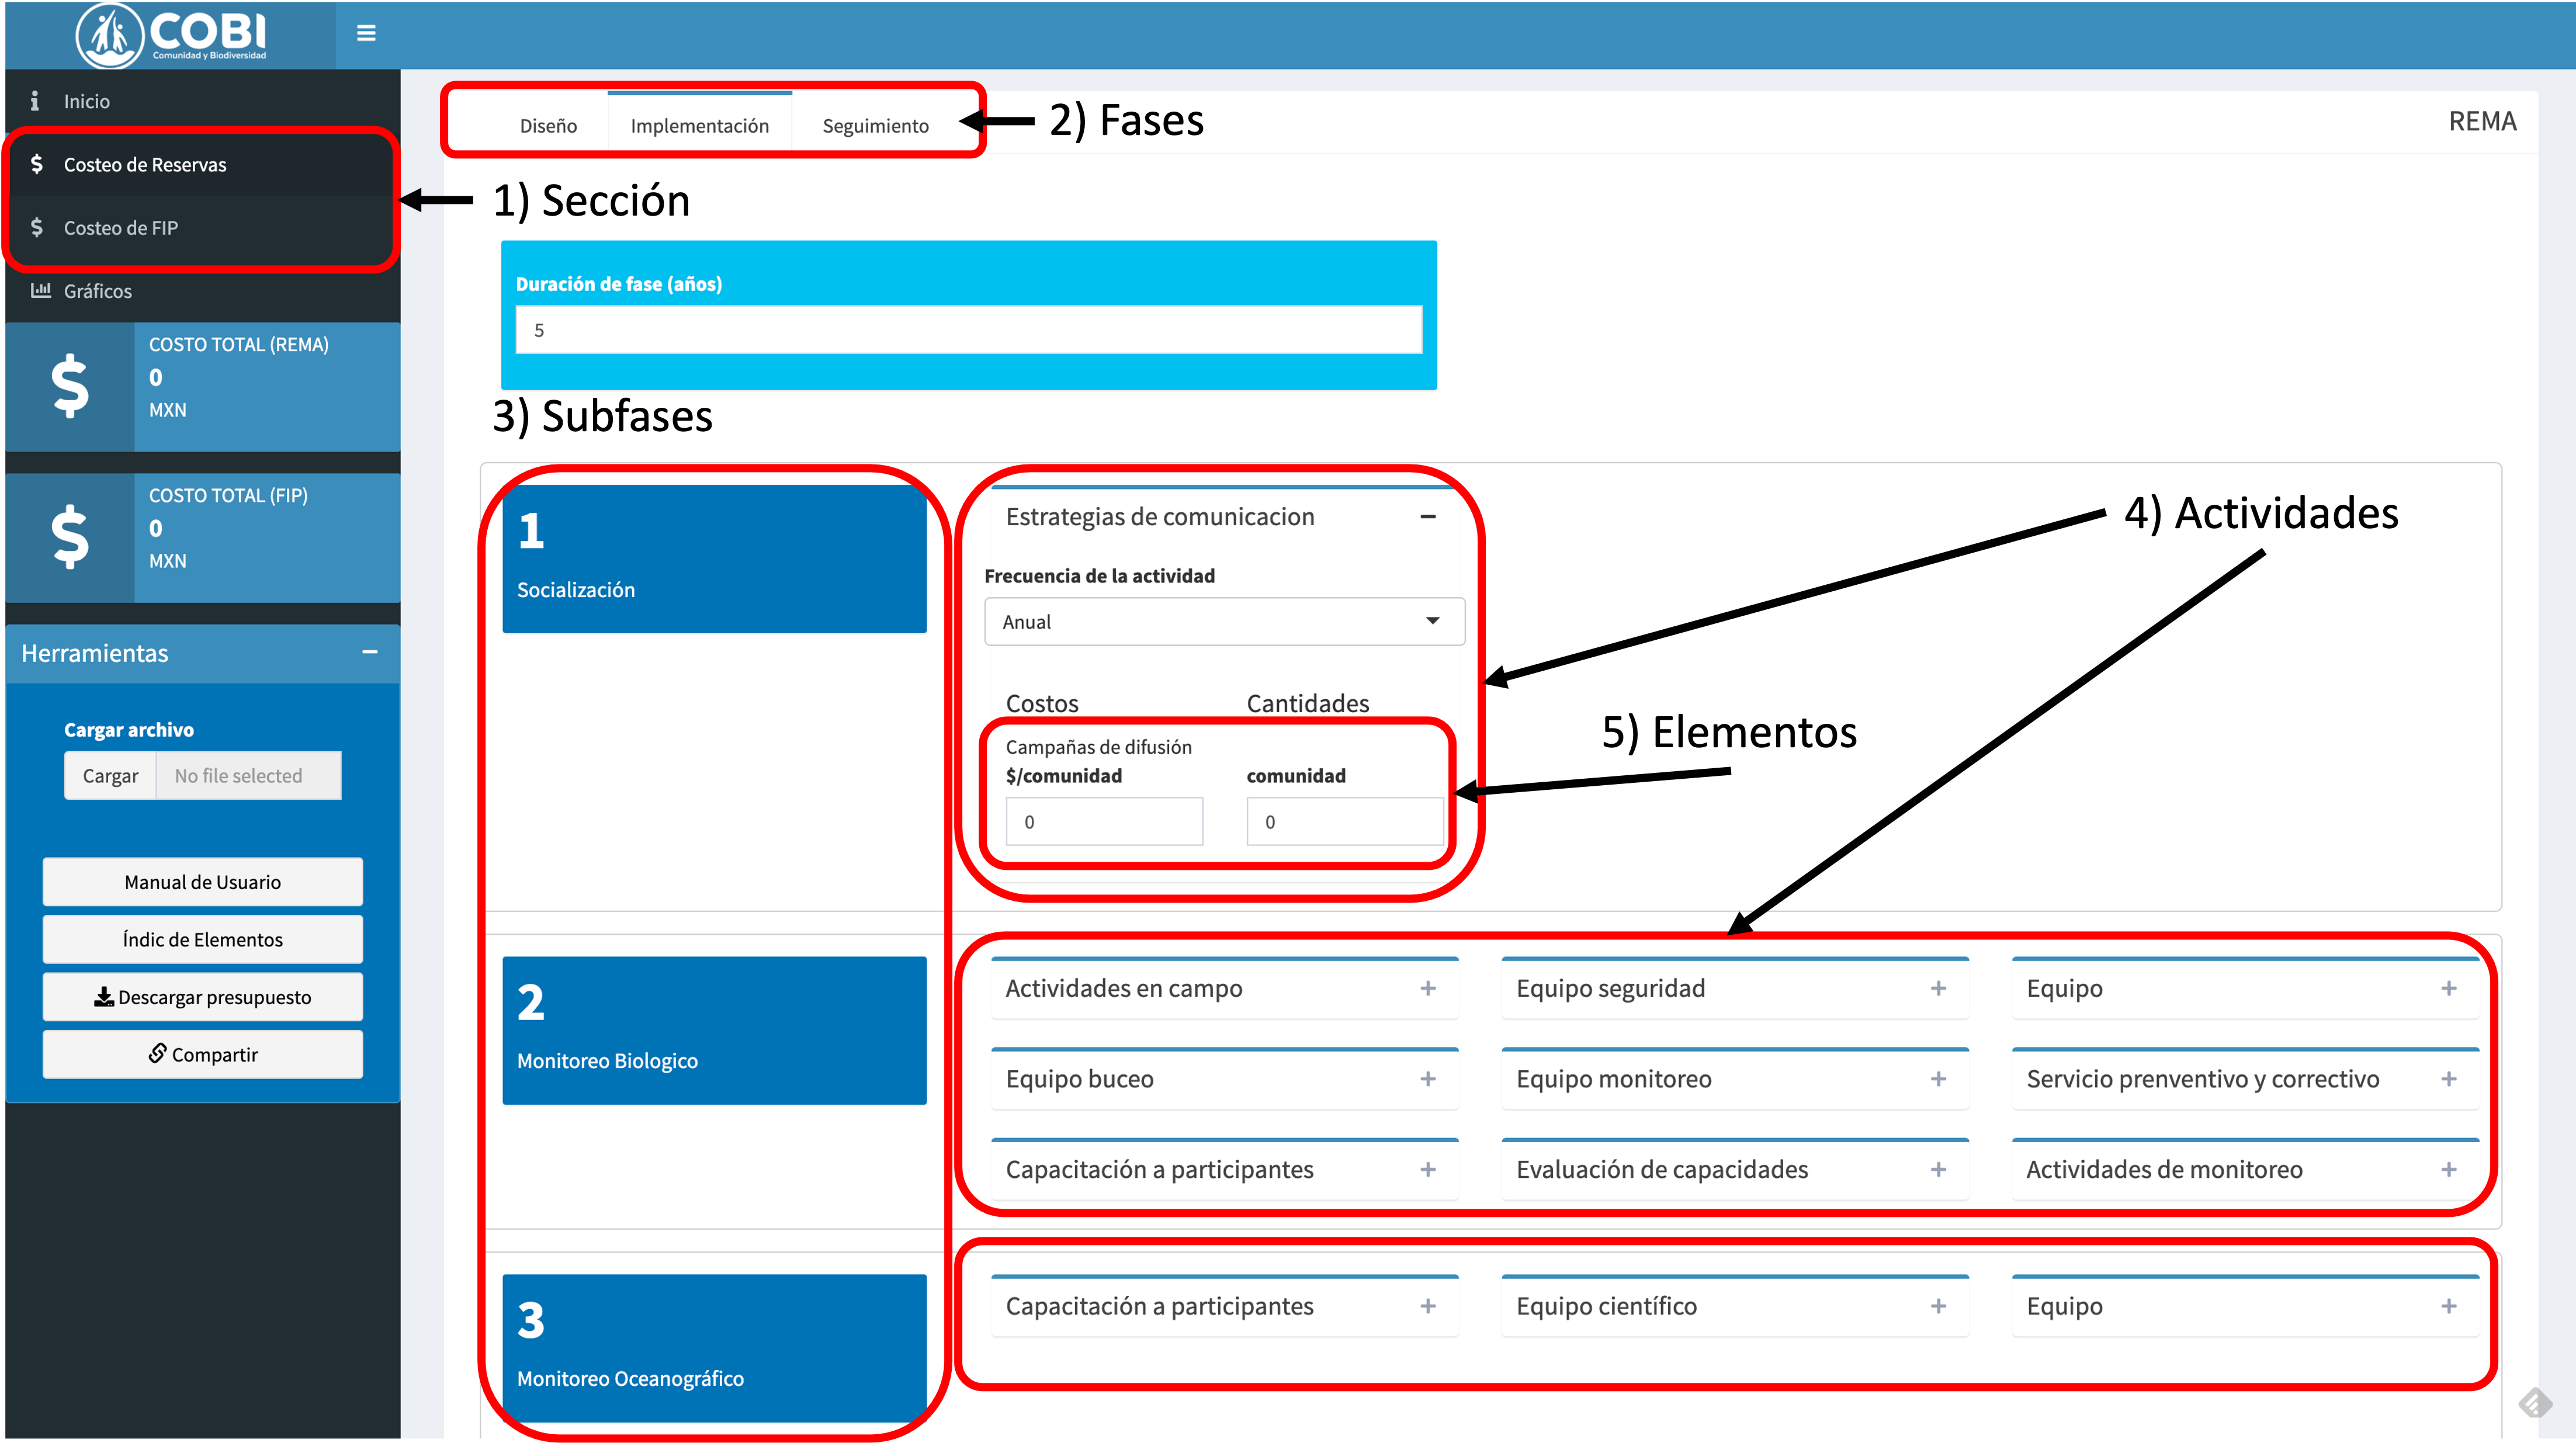
\includegraphics{images/jerarquia.png}
\caption{\label{fig:filling-page}Página de llenado de datos en la aplicación web.}
\end{figure}

La fase de diseño de reservas marinas se subdivide en cuatro subfases, indicadas por los bloques azules del lado izquierdo. En este caso, el diseño de una reserva marina requiere de Socialización, Definicion de Objetivos, Elaboración de un Estudio Técnico Justificativo, y ``Otros'' (otros costos que el usuario puede incluir). Como dijimos en la sección \ref{estructura}, las subfases se dividen en actividades. Por ejemplo, la subfase de socialización cuenta con una única actividad: ``Reuniones para presentar información de ZRP''. Al hacer ``click'' en el signo de \textbf{+} a la derecha del título de la actividad, la aplicación despliega la lista de elementos a costear (Fig. \ref{fig:elements}), así como la frecuencia de la actividad. Aprenderemos más sobre el llenado de un presupuesto en el capítylo \ref{llenado}.

\begin{figure}
\centering
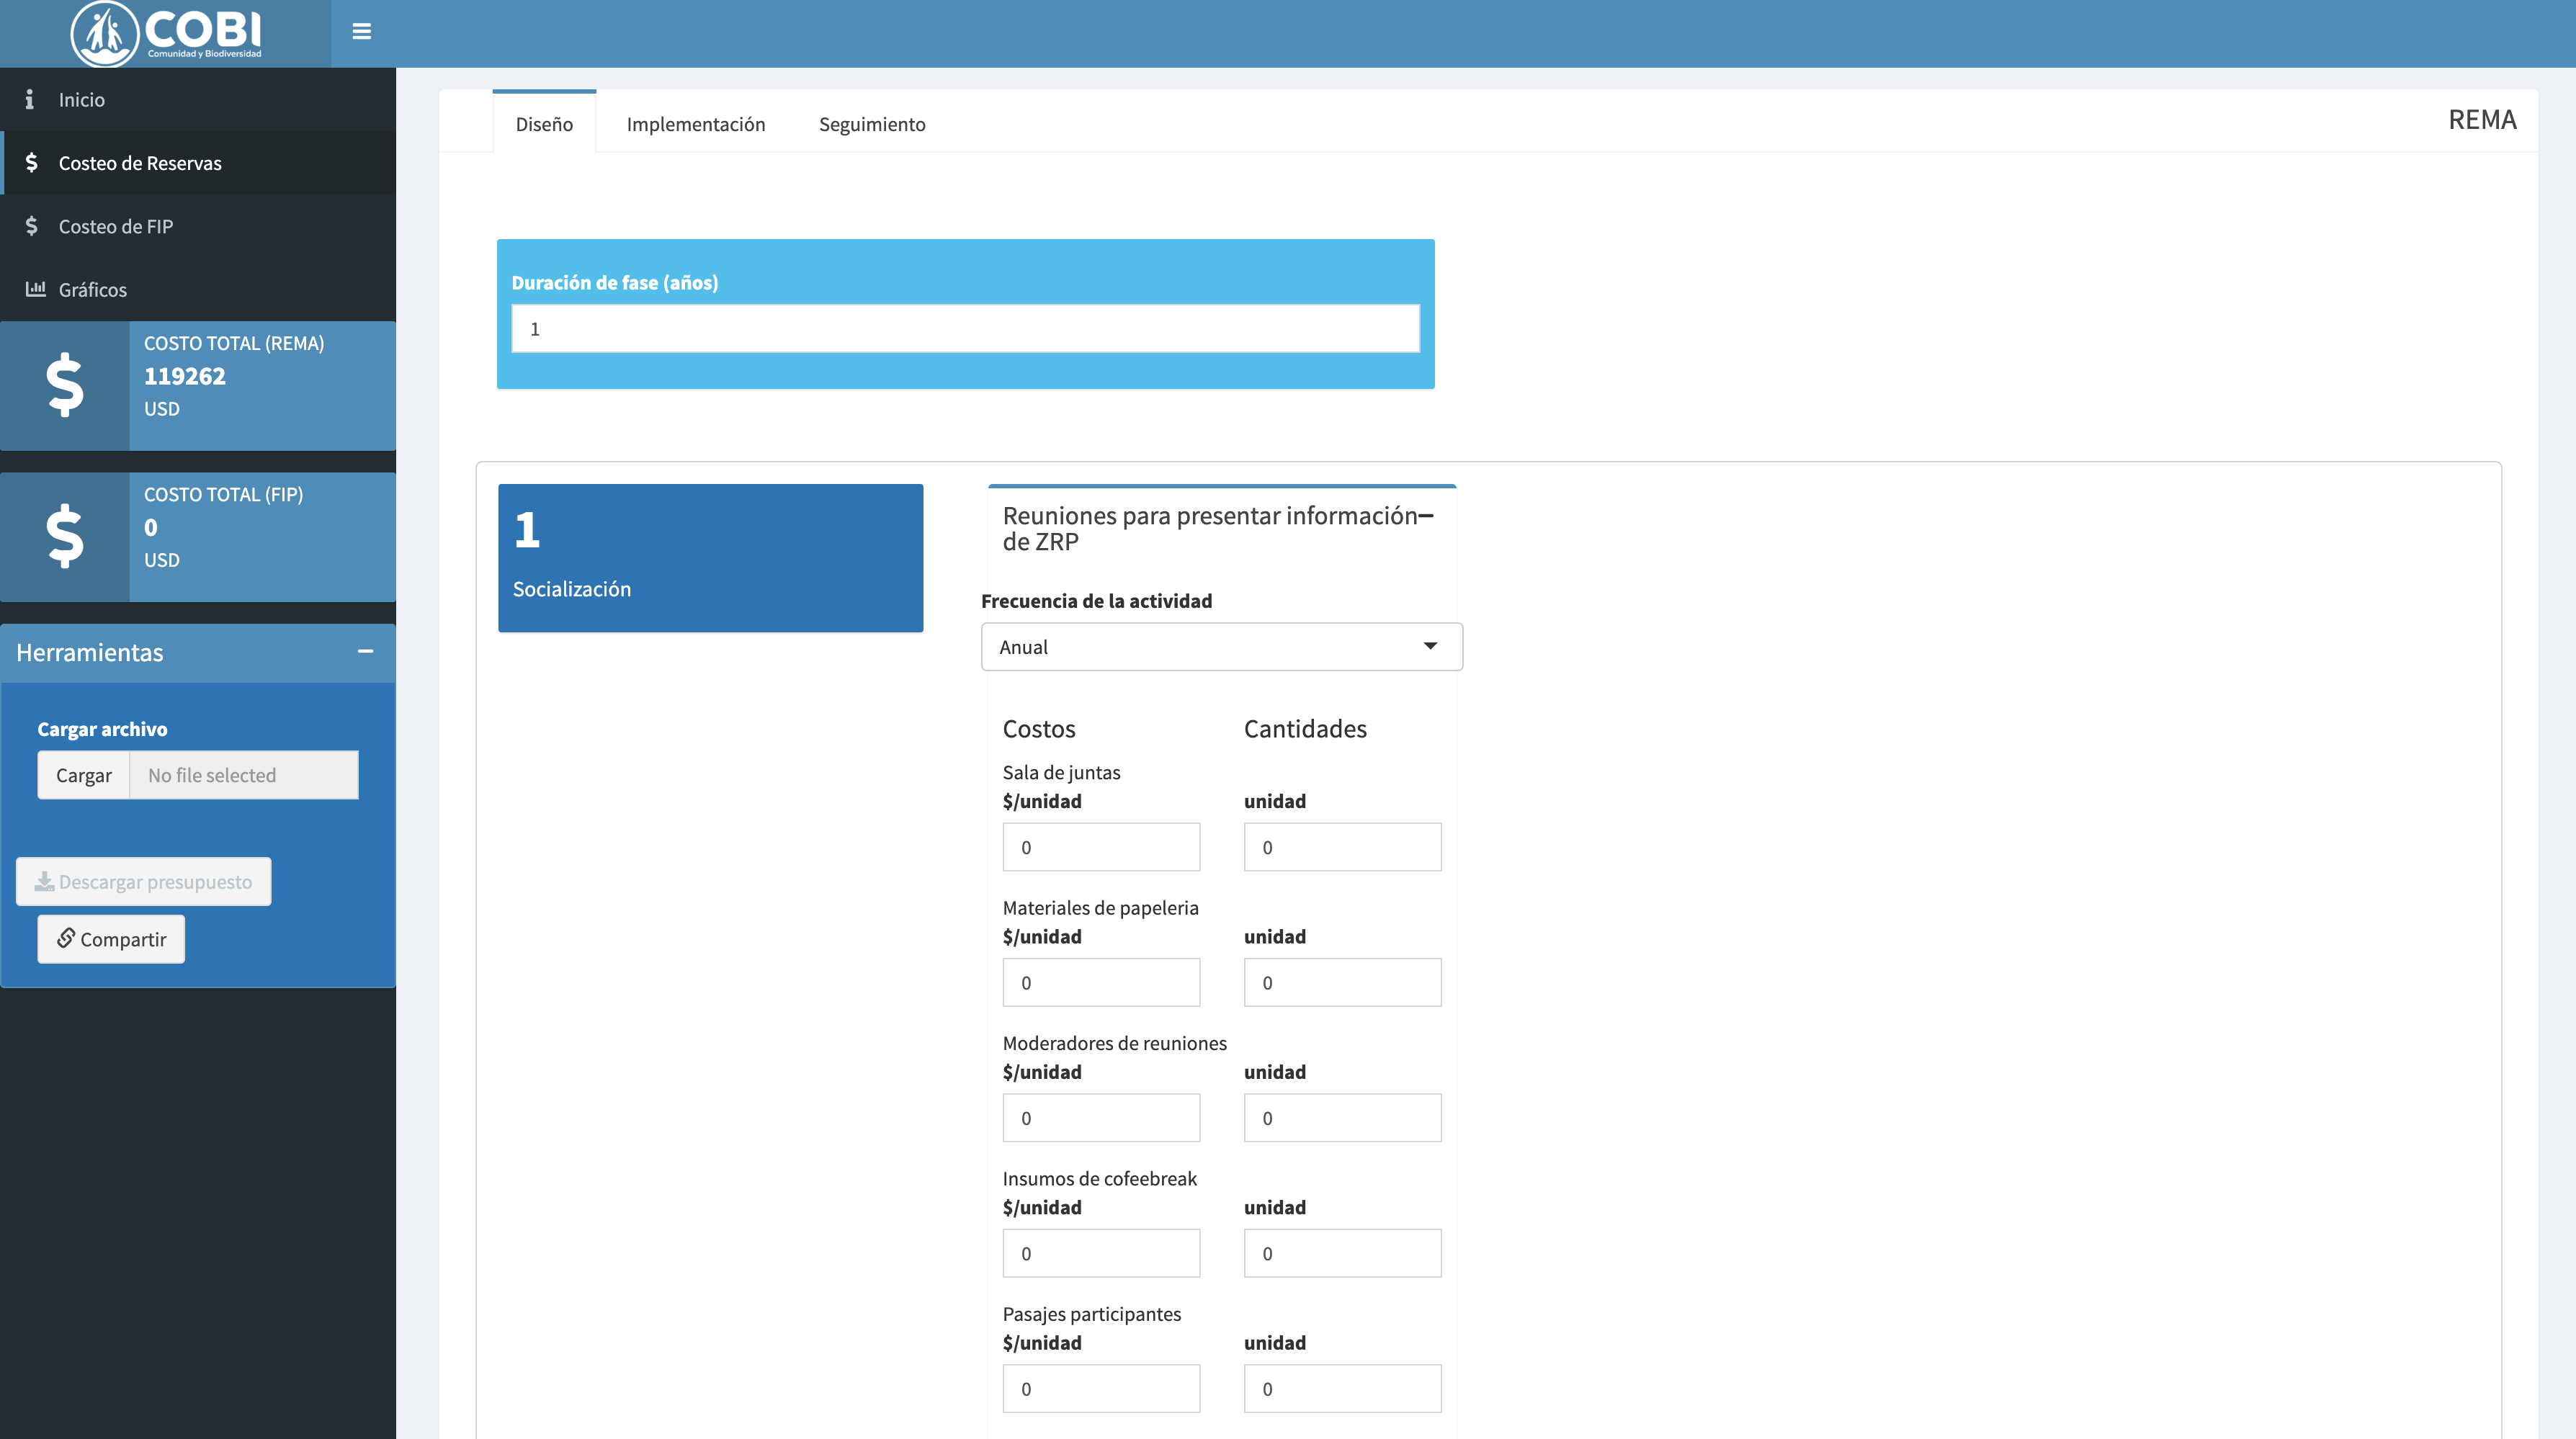
\includegraphics{images/Screen Shot 2022-07-25 at 3.08.10 PM.png}
\caption{\label{fig:elements}Elementos para la actividad de `Reuniones para presentar información de ZRP'.}
\end{figure}

La figura \ref{fig:viewing-page} muestra el último área de trabajo, donde podrás visualizar el presupuesto. Además, contiene una nueva característica de esta versión de la aplicación: Te permite dividir el presupuesto entre diferentes actores, y anticipar el monto de sus contribuciones. Aprenderemos más a detalle sobre esta sección en el capítulo \ref{explorar}.

\begin{figure}
\centering
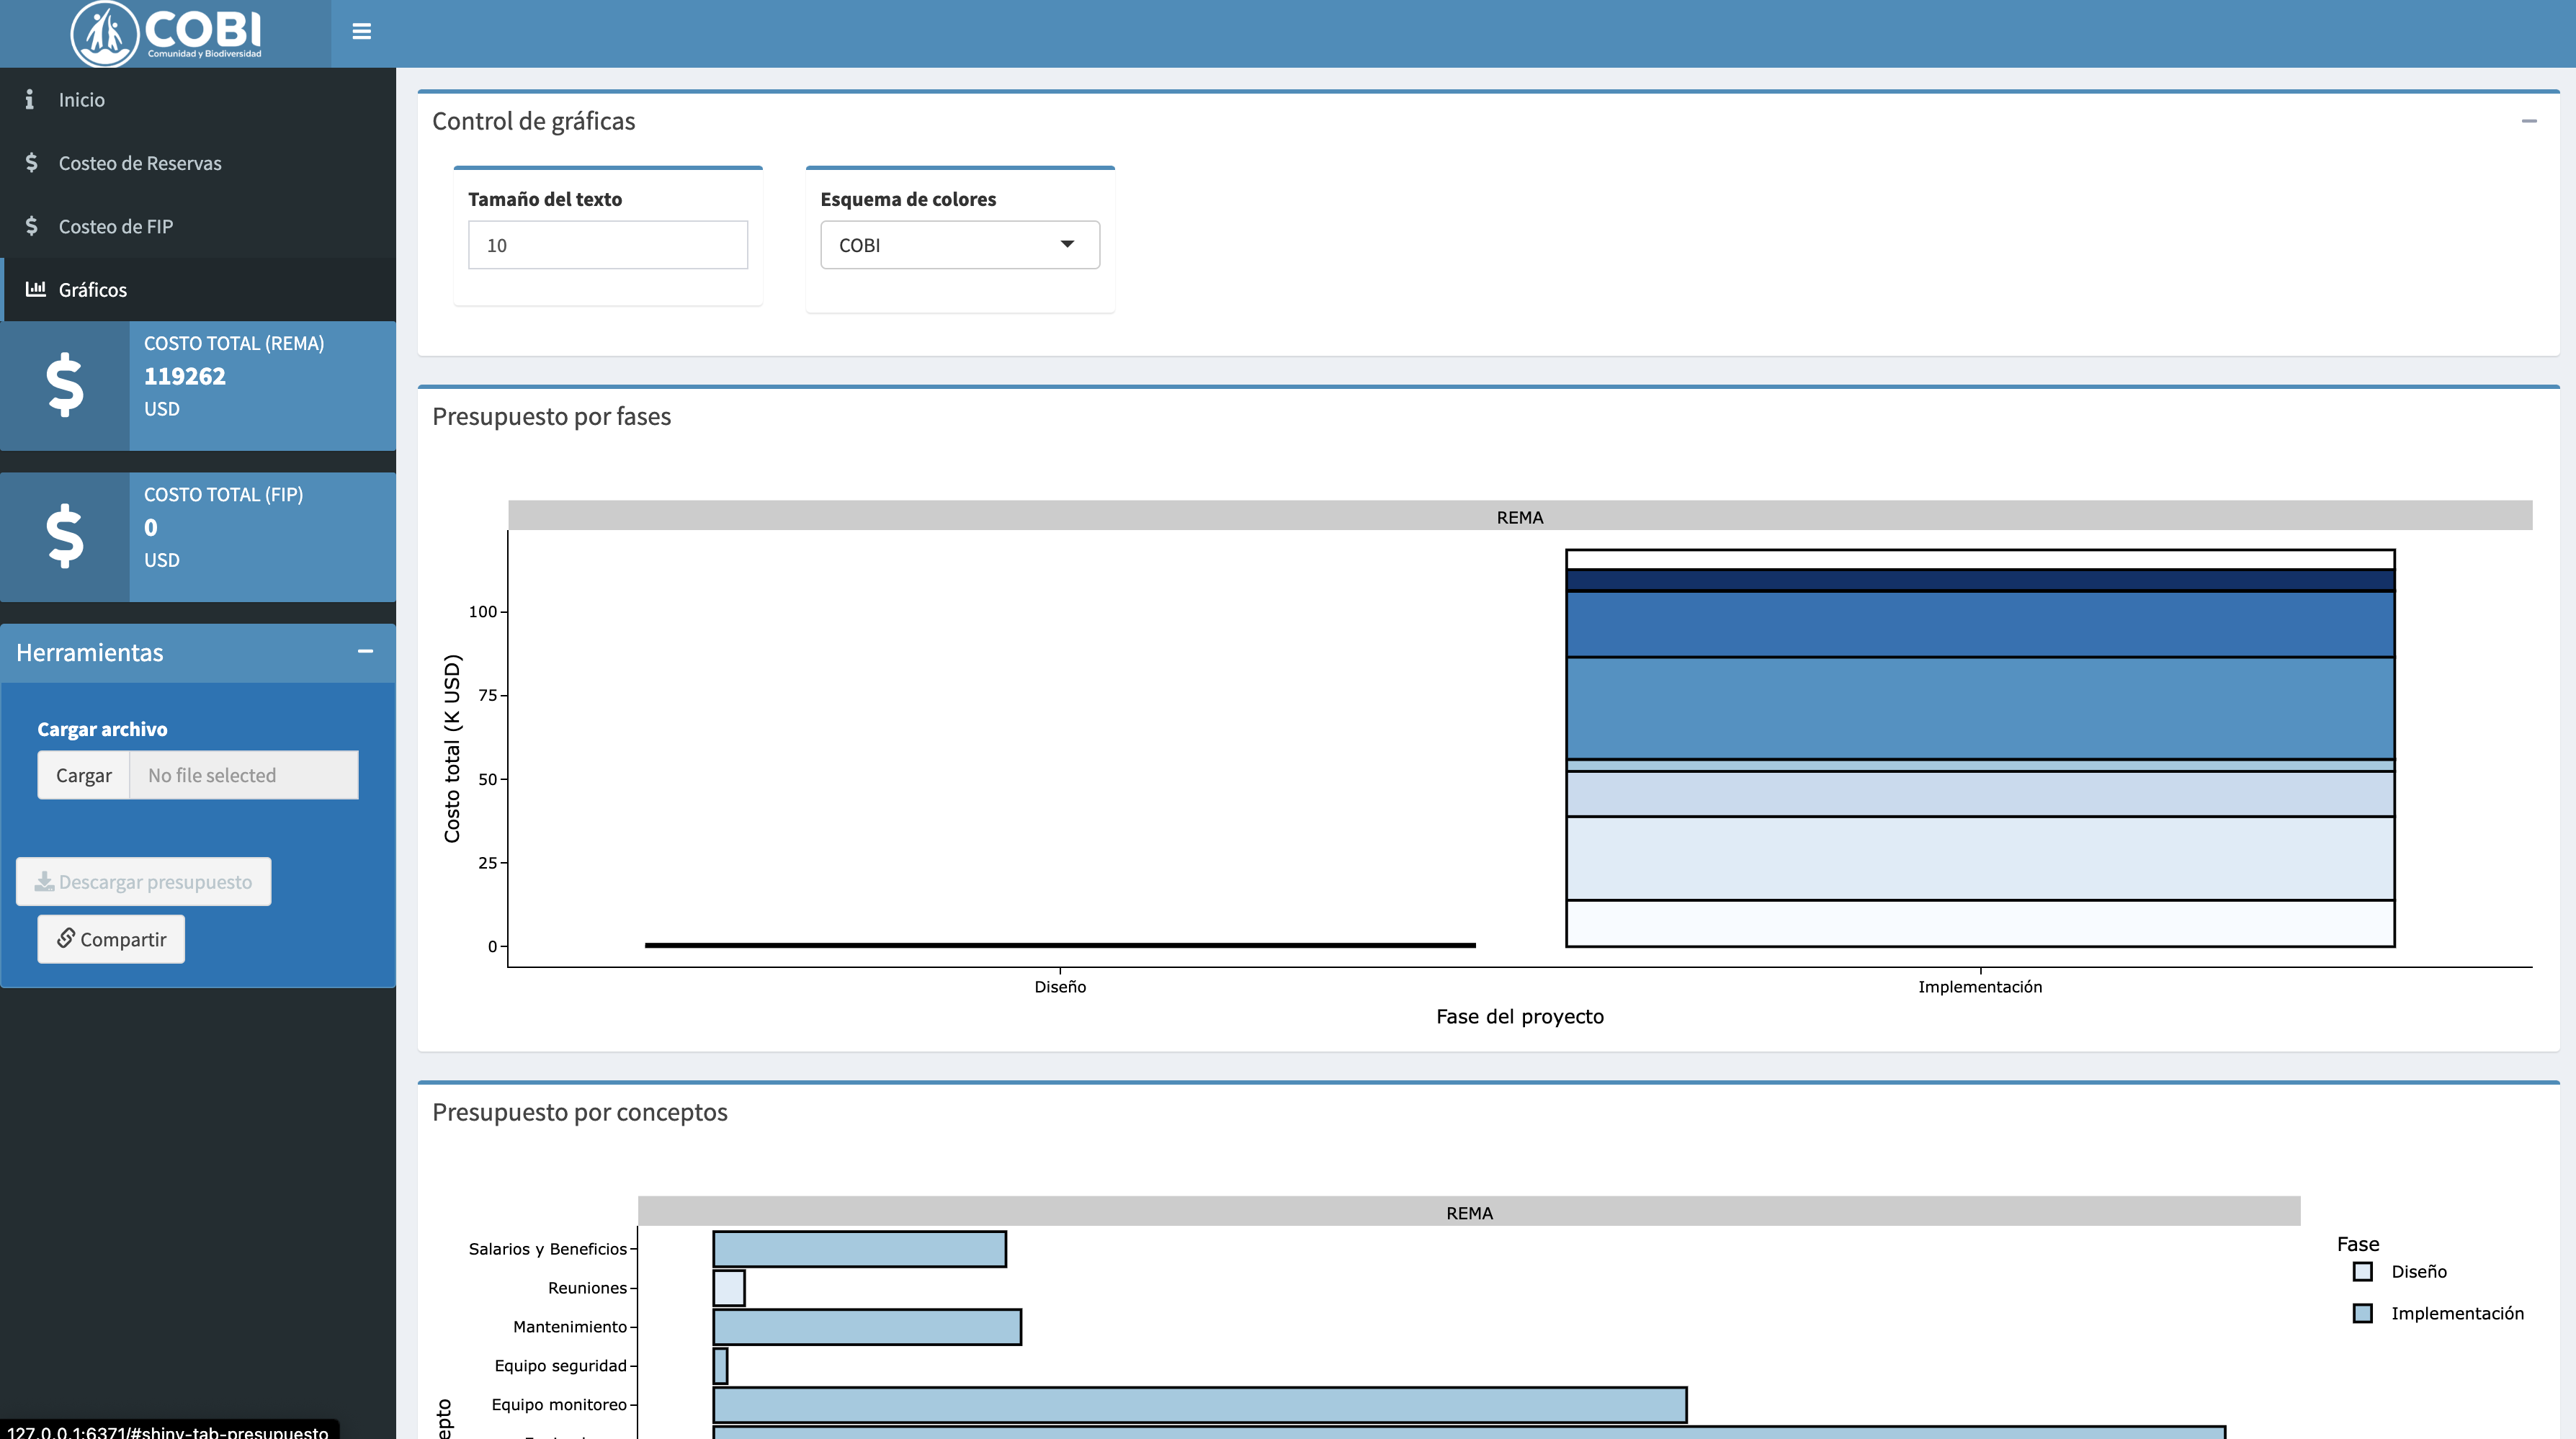
\includegraphics{images/Screen Shot 2022-07-25 at 2.56.18 PM.png}
\caption{\label{fig:viewing-page}Página de exploración de presupuesto en la aplicación web.}
\end{figure}

\hypertarget{llenado}{%
\chapter{Llenado de datos}\label{llenado}}

En este capítulo exploramos la interfaz para el llenado de datos. Recuerda que el presupuesto sigue una regla de jerarquías descrita en la sección \ref{estructura}. El primer ejercicio se enfocará en la fase de diseño de reservas marinas. El segundo ejemplo se enfocará en la fase de implementación de un FIP. En ambos casos, utiizaremos un recuadro rojos obre las capturas de pantall para resaltar el módulo en la que estamos trabajando.

\hypertarget{rema}{%
\section{Ejemplo de REMA}\label{rema}}

\textbf{Paso 1 - } Selecciona la pestaña de ``Costeo de Reservas'' (Fig. \ref{fig:rem-dis-1}). Auomáticamente, la app te muestra la fase de diseño (primer pestaña del área de trabajo).

\begin{figure}
\centering
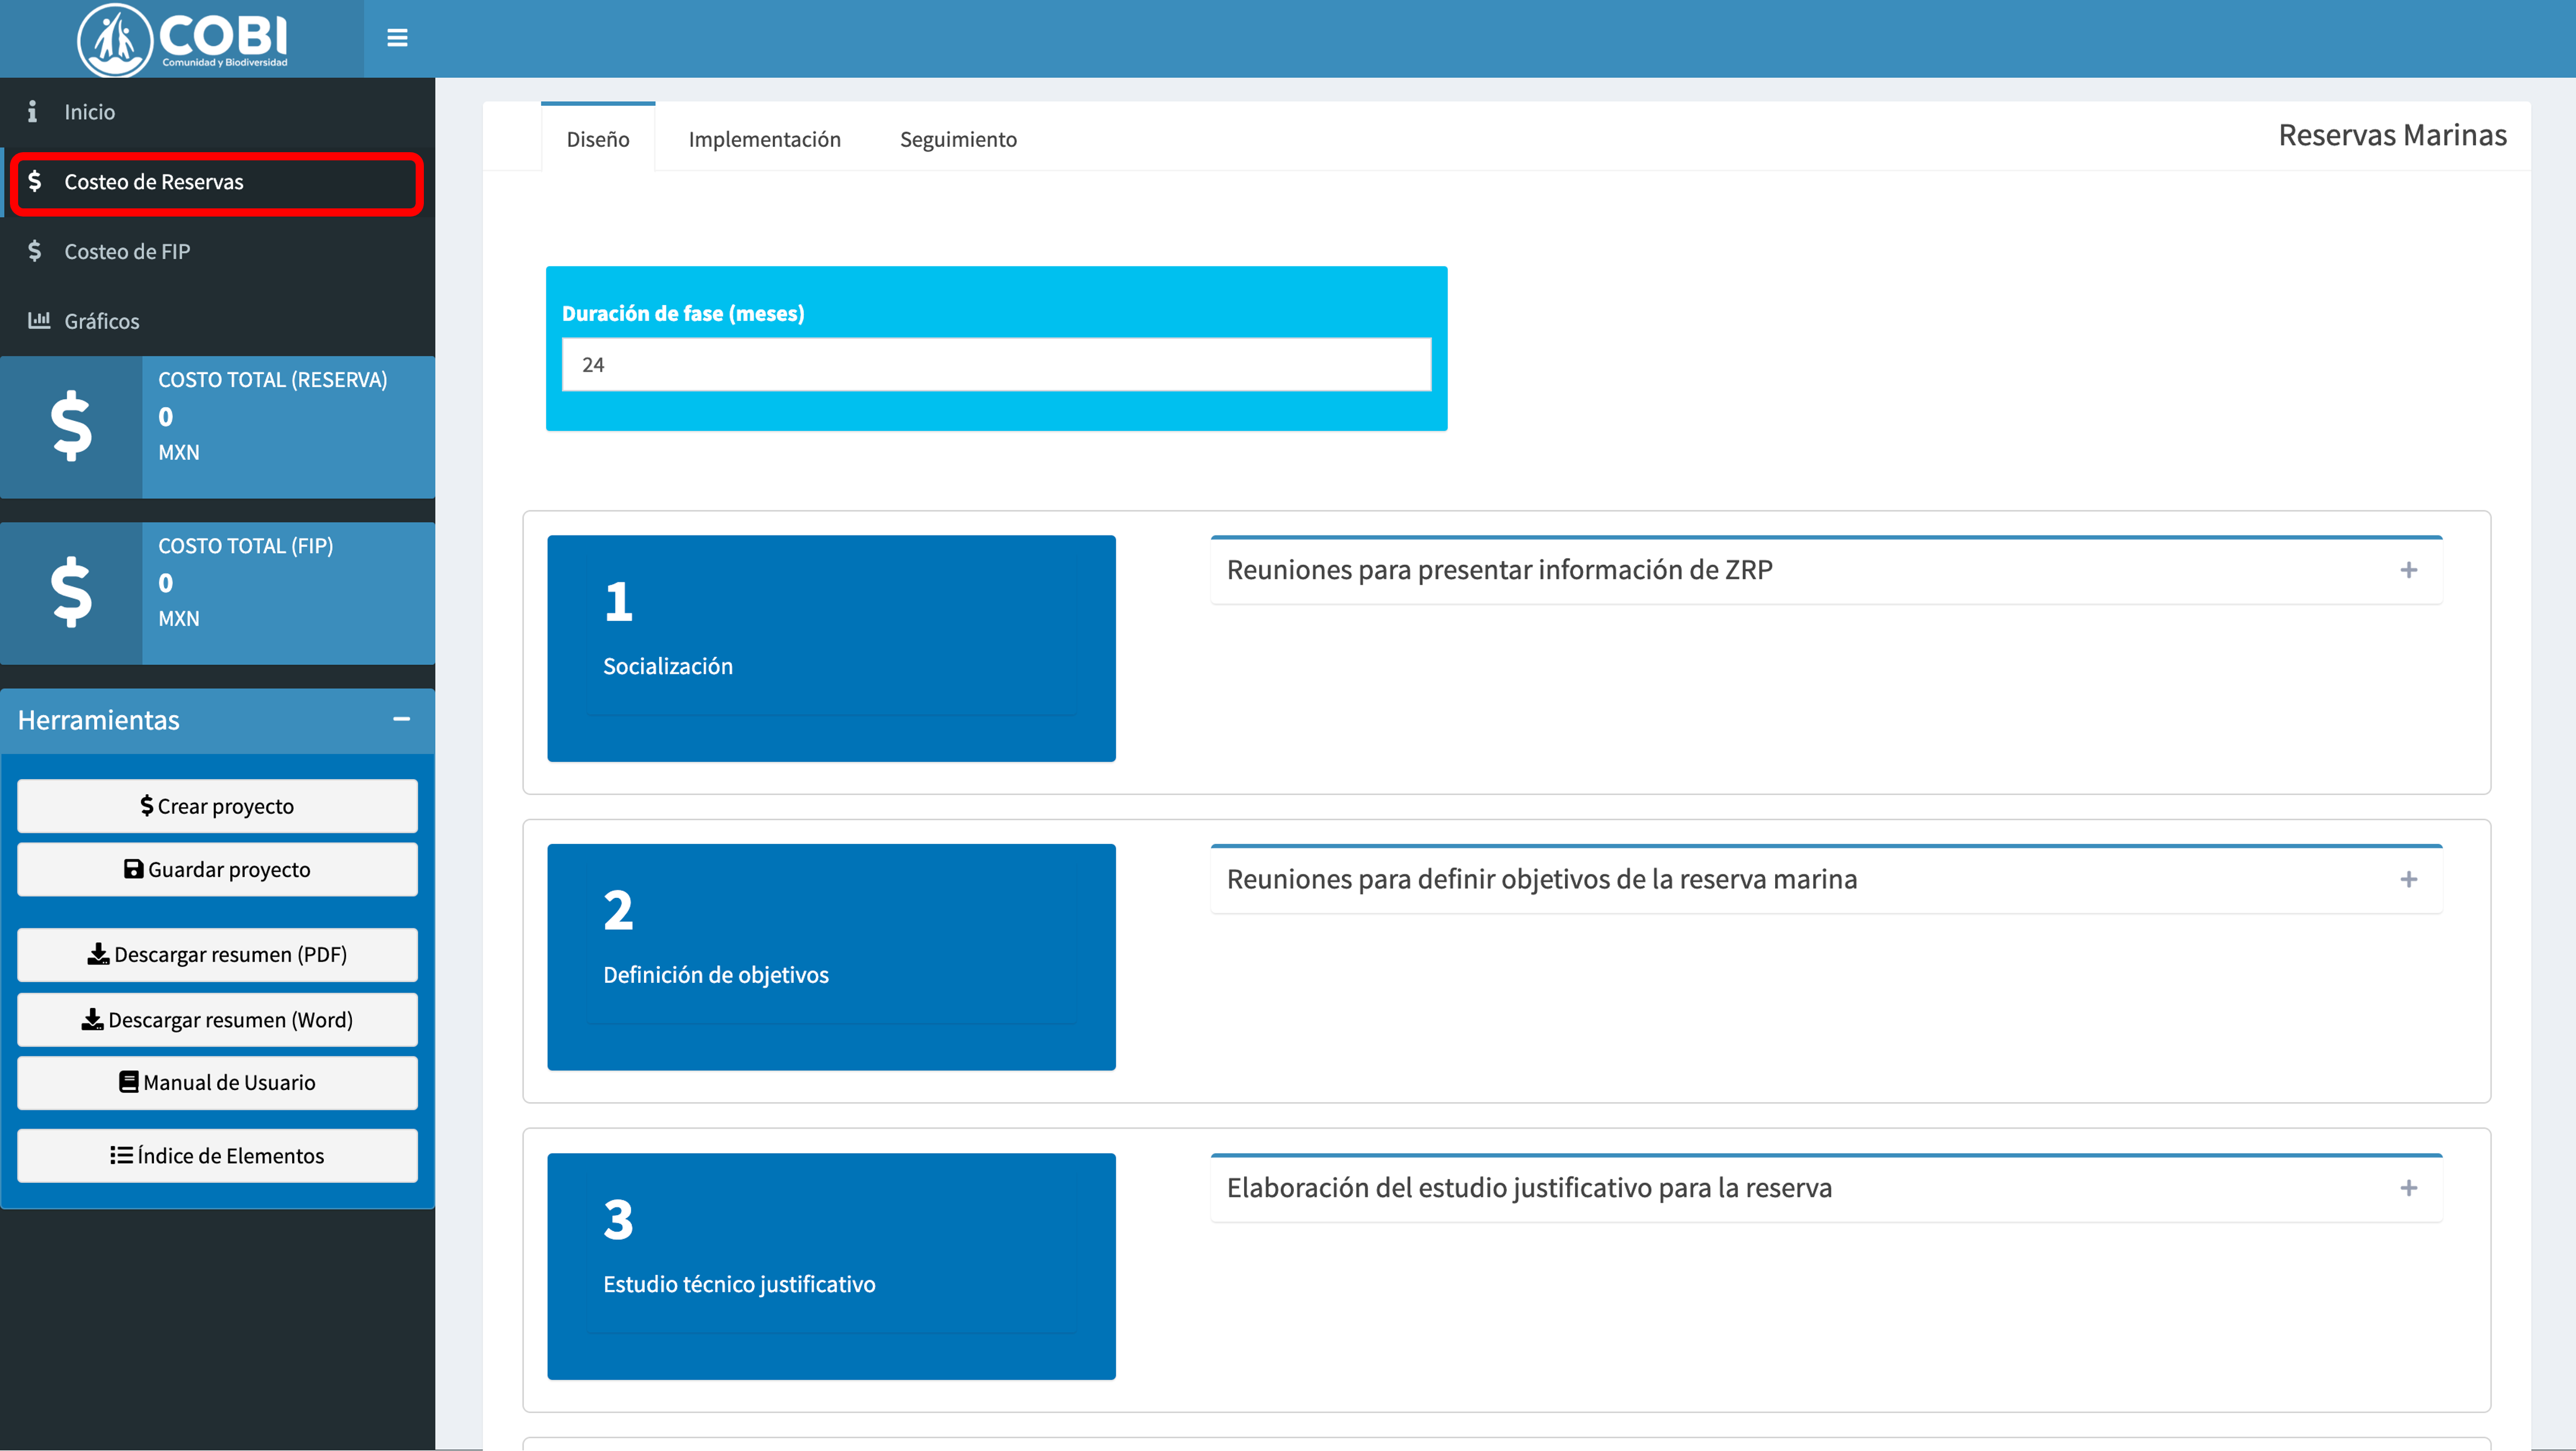
\includegraphics{images/rema_dis_1.png}
\caption{\label{fig:rem-dis-1}Interfaz de usuario con la sección de Costeo de Reservas seleccionada}
\end{figure}

\textbf{Paso 2 - } Actualiza la duración de la fase de diseño a 2 años en el recuadro azul sobre las cuatro subfases (Fig \ref{fig:rem-dis-2}).

\begin{figure}
\centering
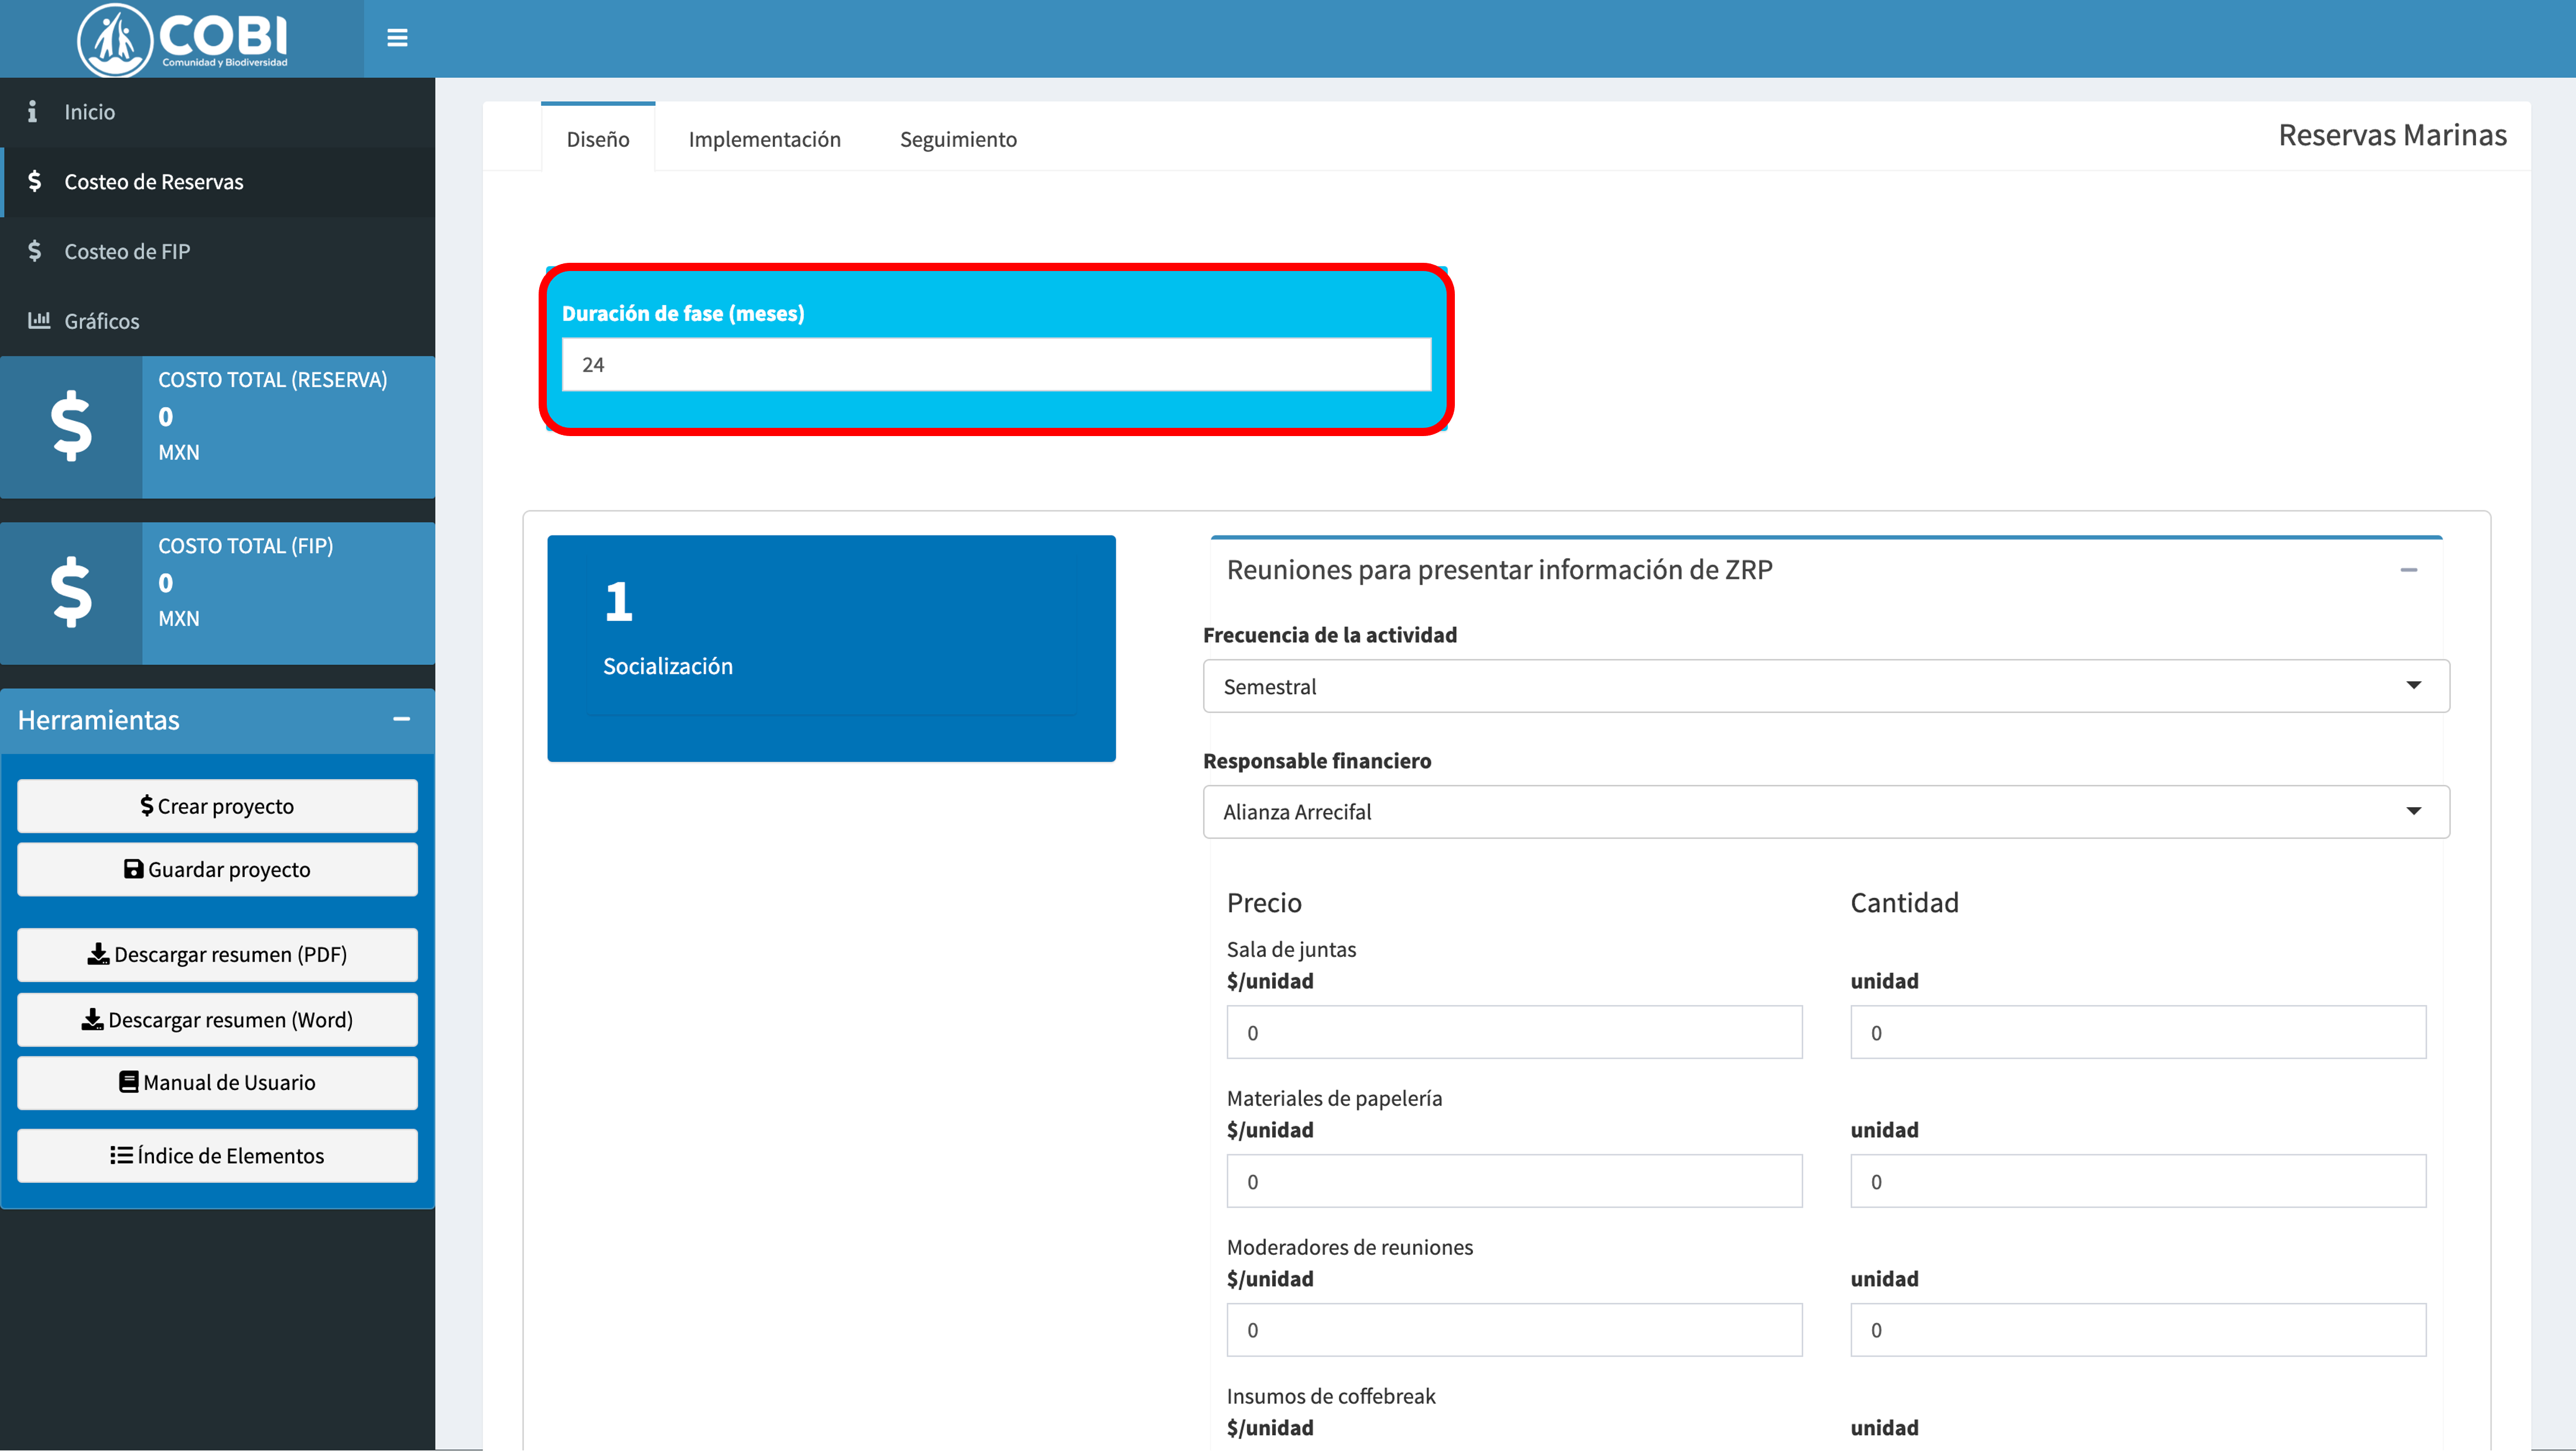
\includegraphics{images/rema_dis_2.png}
\caption{\label{fig:rem-dis-2}Modificación de la duración de fase.}
\end{figure}

\textbf{Paso - 3 } Para llenar la subfase de Socialización, haz click en el simbolo de \textbf{+} en la esquina superior derecha cada actividad. Esto te mostrará todos los elementos que corresponden a esta actividad (Fig \ref{fig:rem-dis-3}).

\begin{figure}
\centering
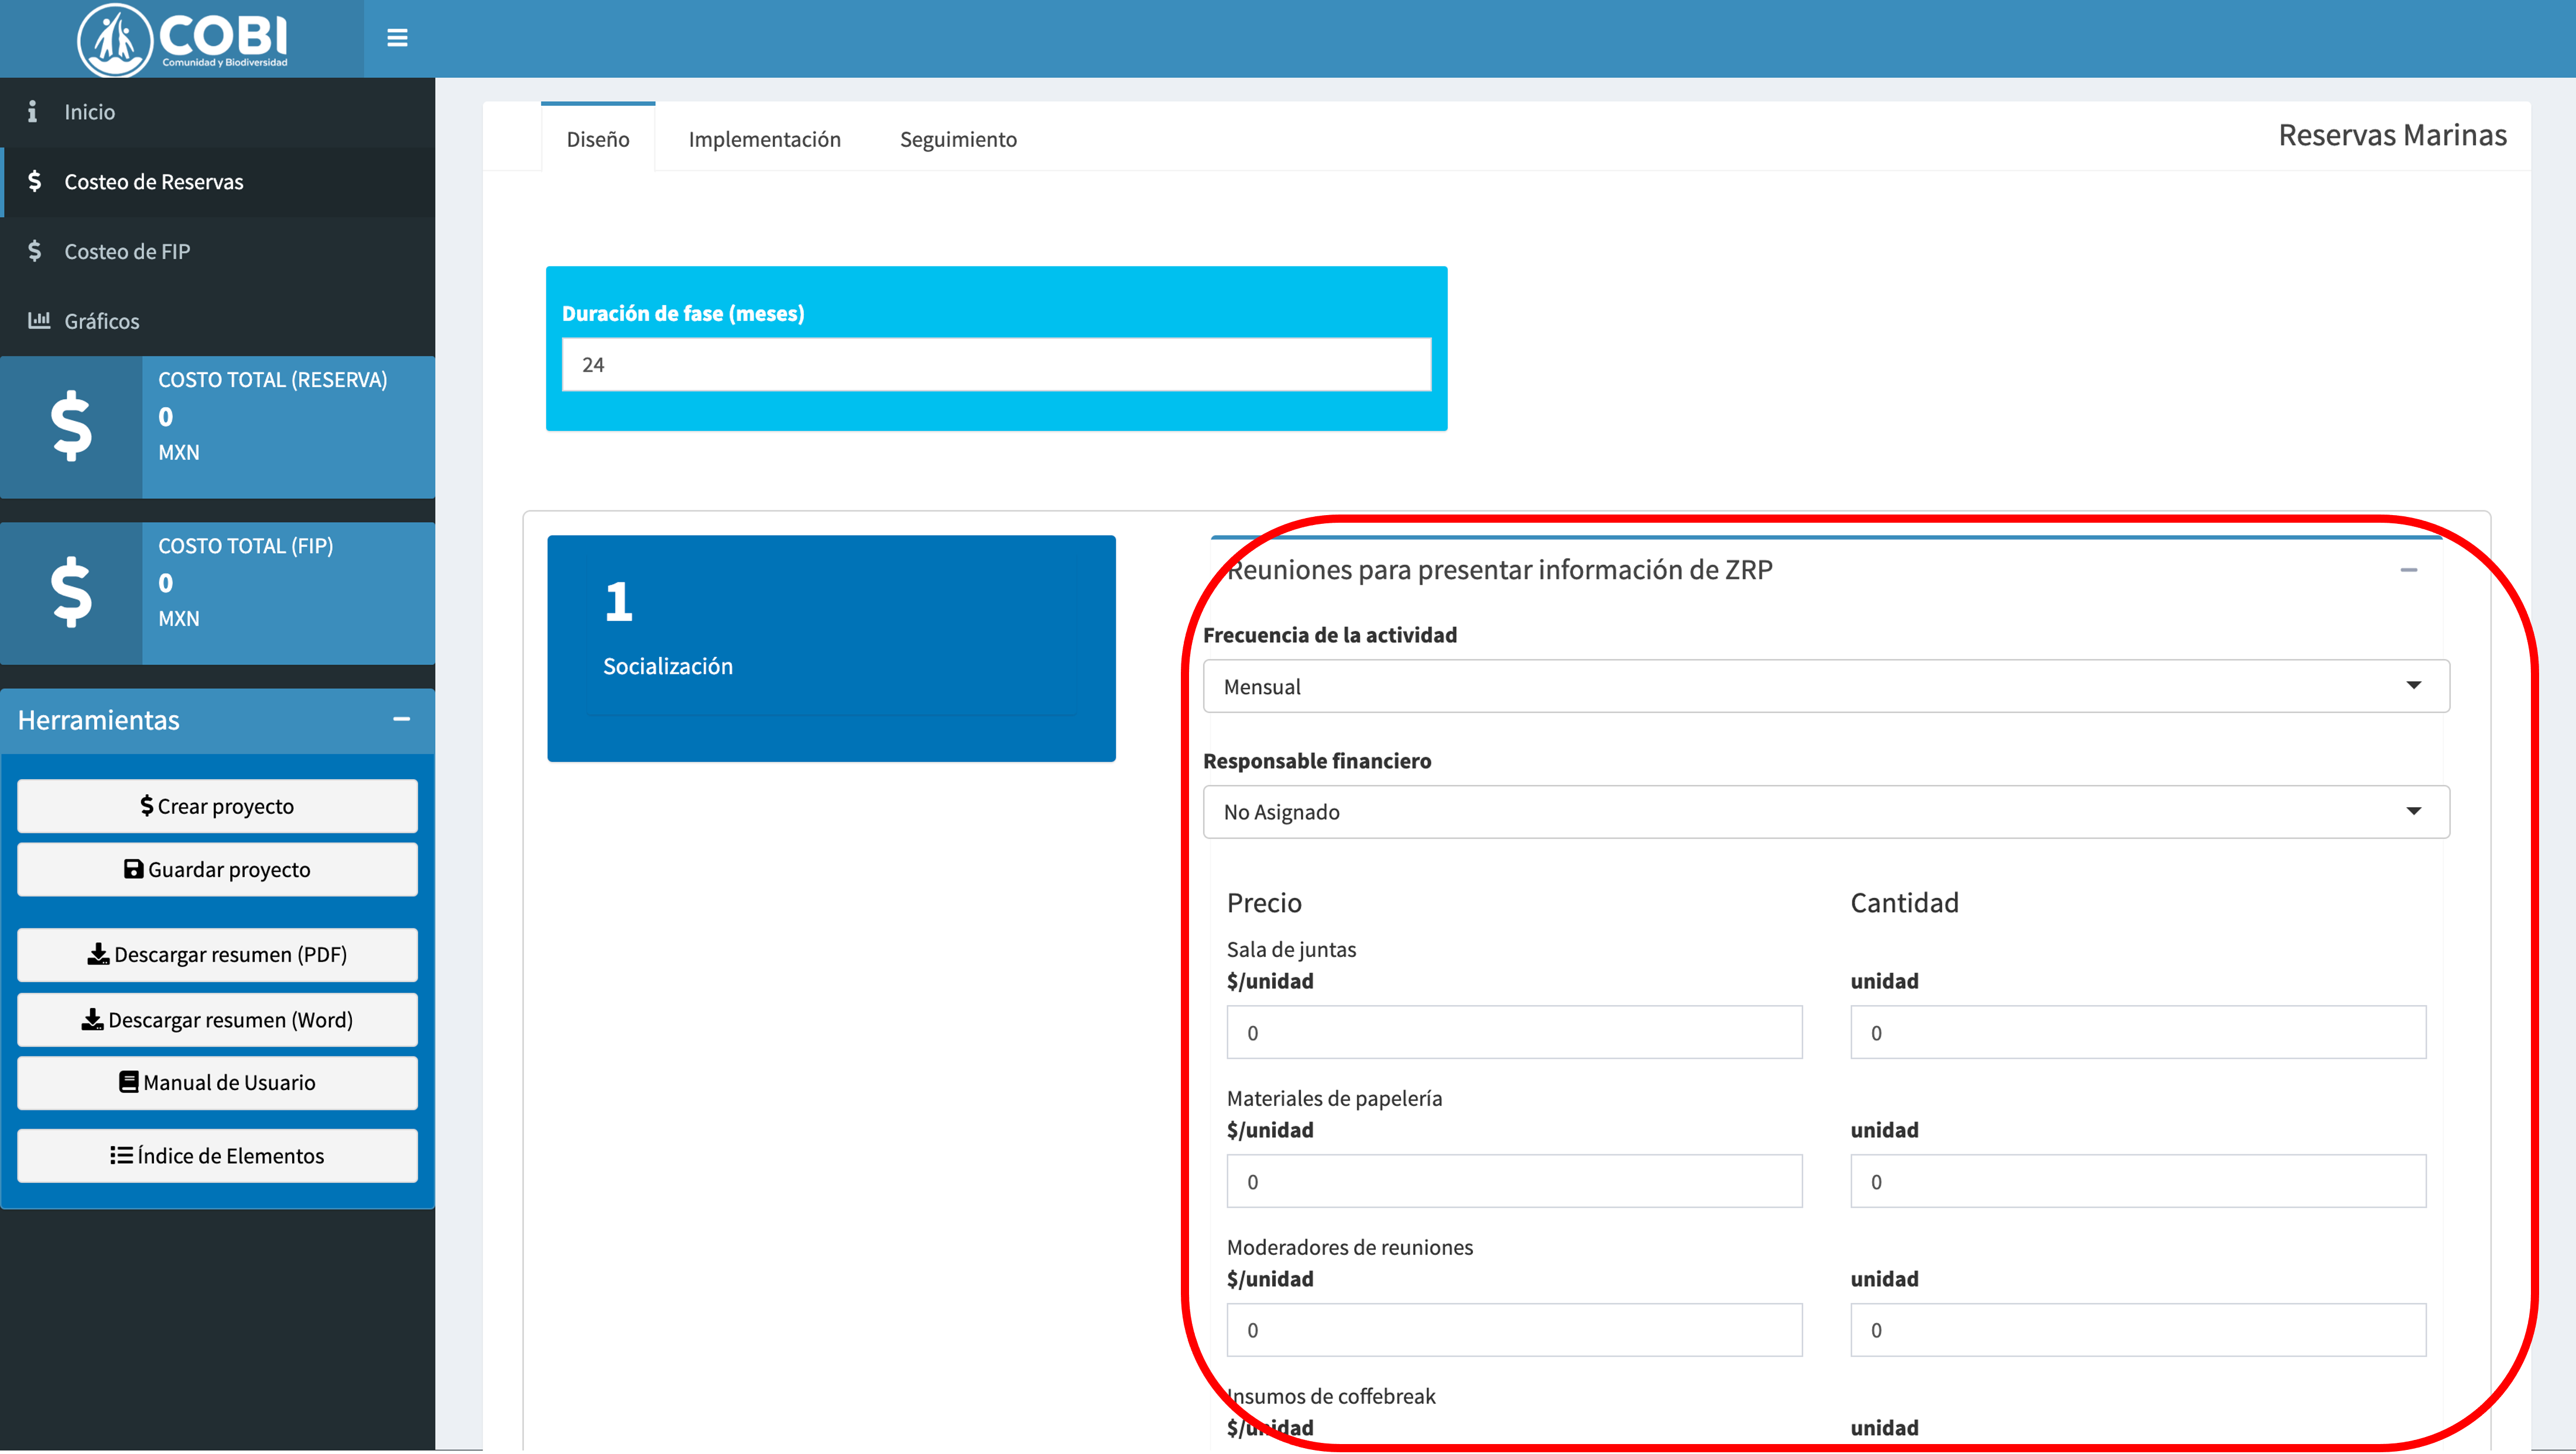
\includegraphics{images/rema_dis_3.png}
\caption{\label{fig:rem-dis-3}Despliegue de una actividad.}
\end{figure}

\textbf{Paso 4 - } Selecciona la frecuencia de las reuniones. En este caso la frecuencia es semestral, pes habrá dos reuniones al año a lo largo de dos años de diseño (Fig \ref{fig:rem-dis-4}).

\begin{figure}
\centering
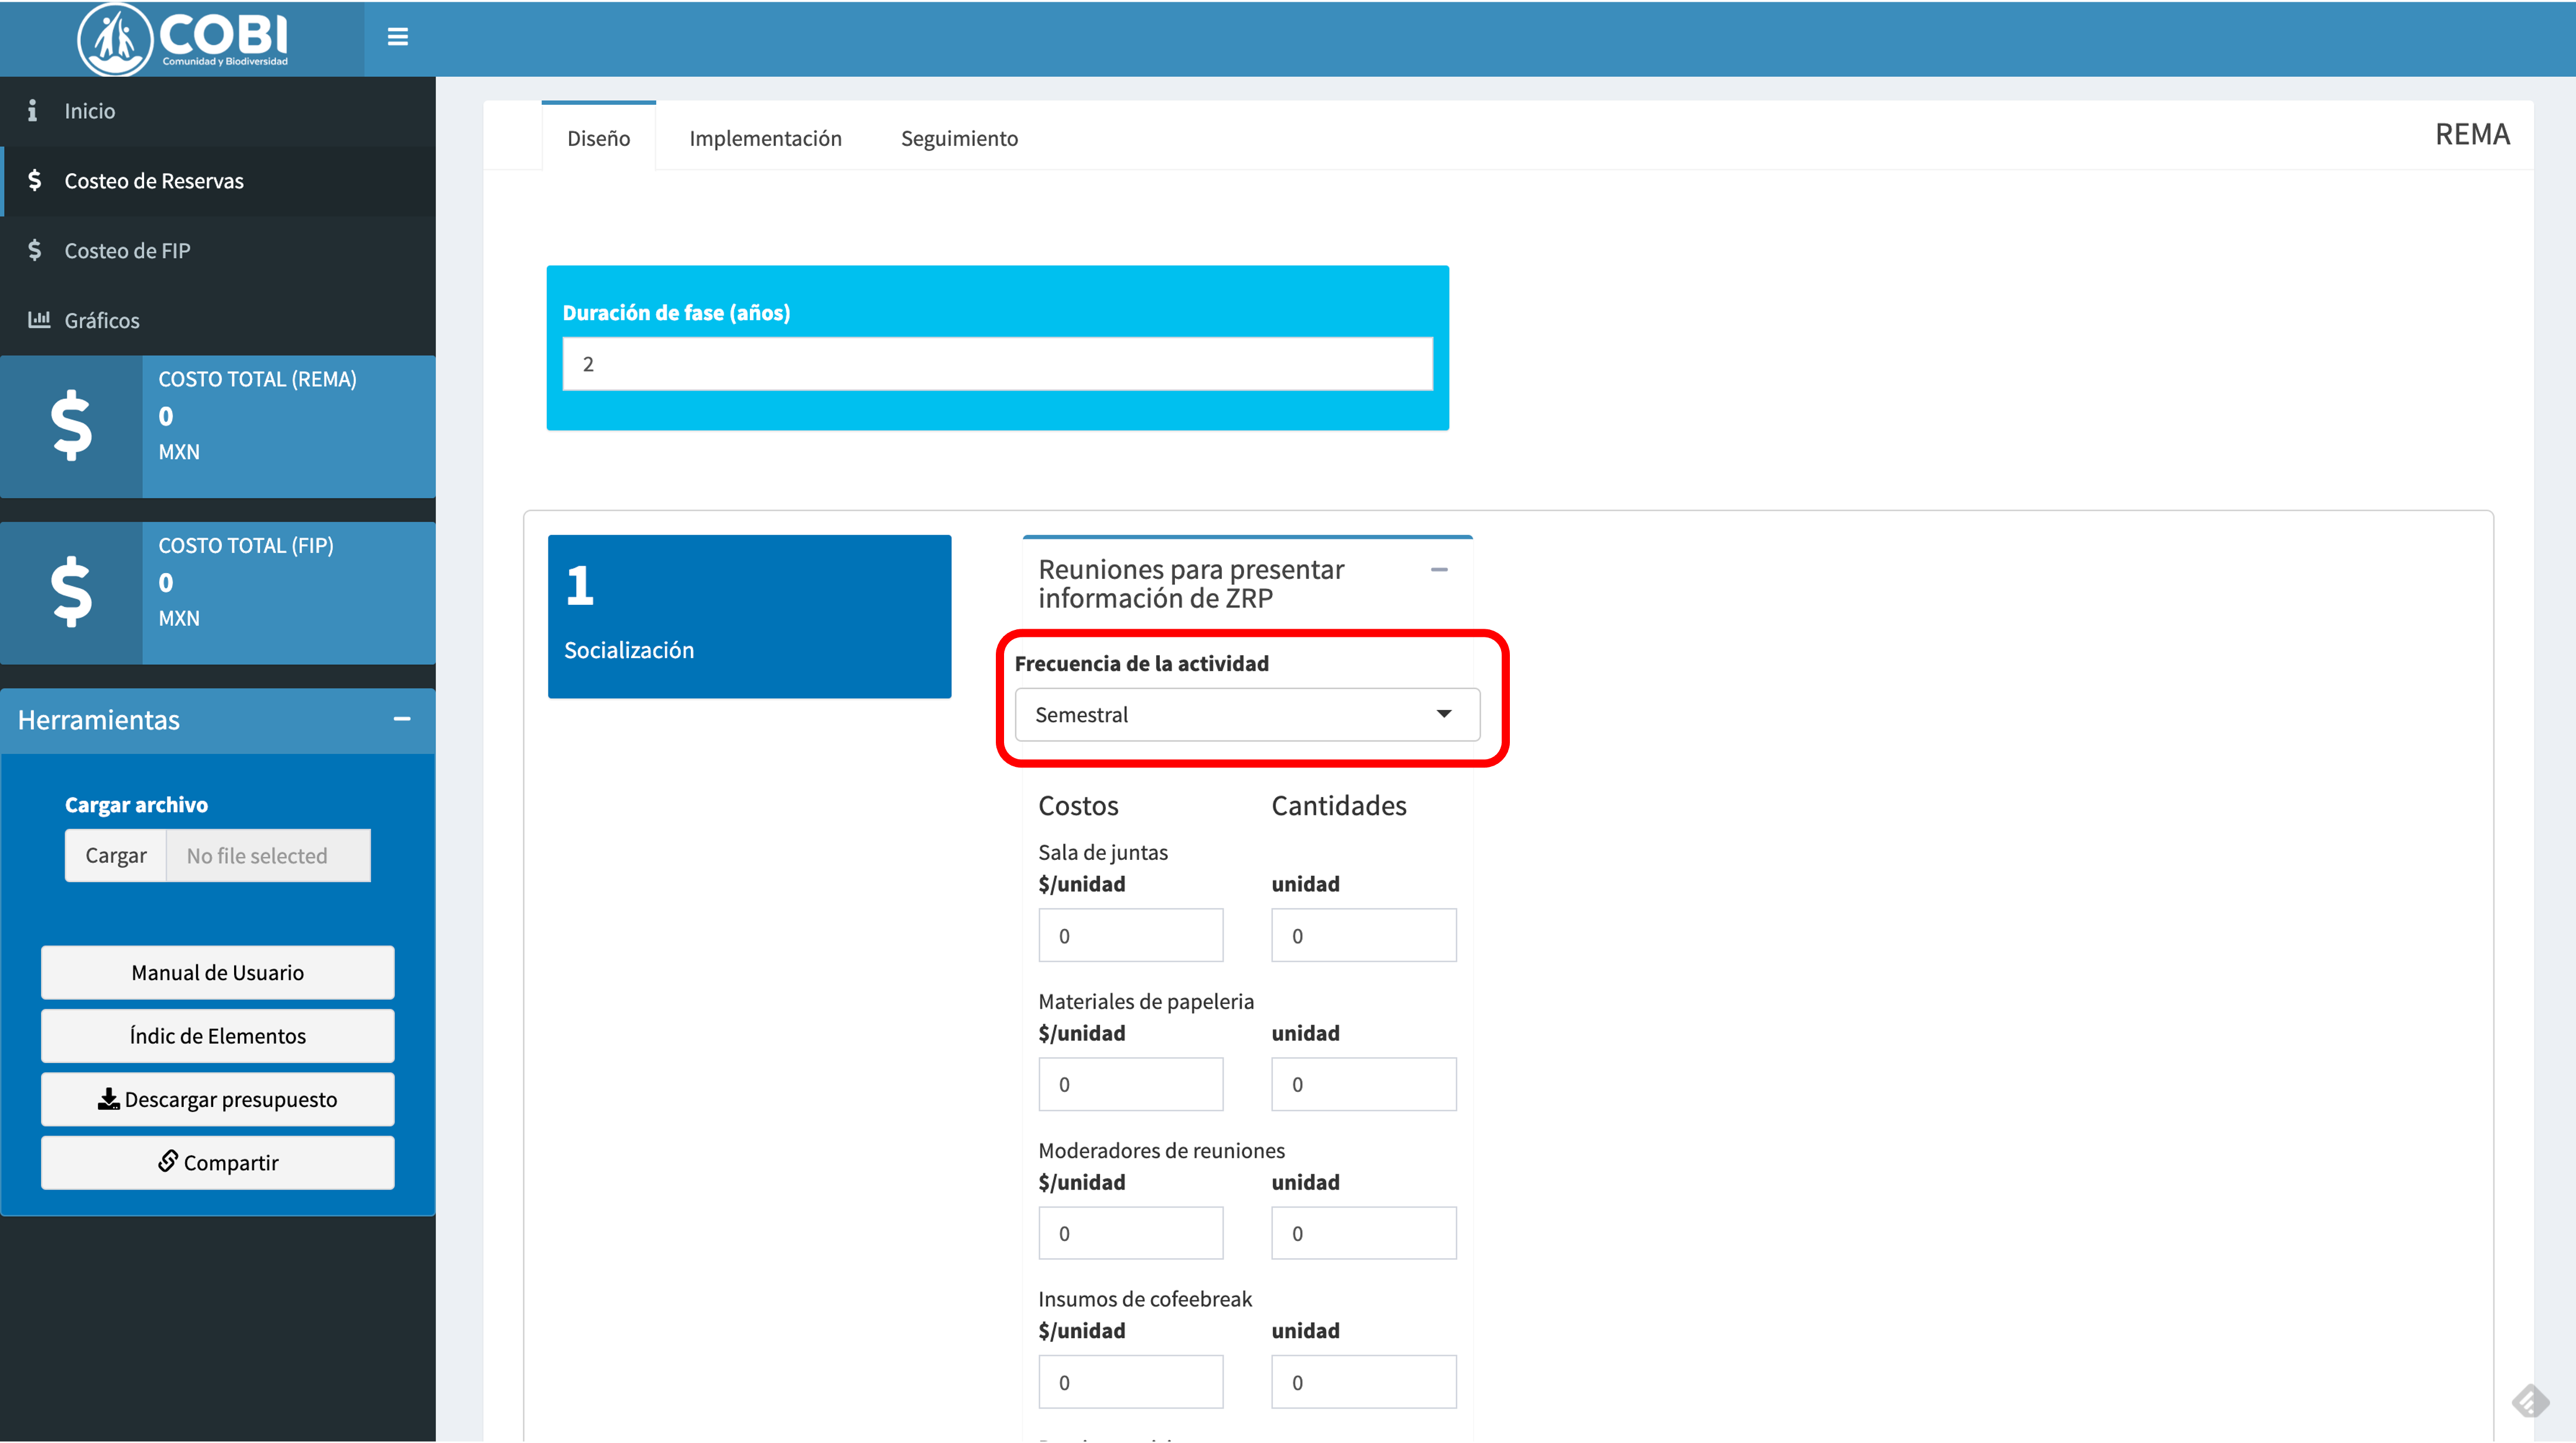
\includegraphics{images/rema_dis_4.png}
\caption{\label{fig:rem-dis-4}Frecuencia de la actividad.}
\end{figure}

\textbf{Paso 5 - } Ingresa los costos y cantidades de cada elemento. En este ejemplo la reunión semestral requiere de \textbf{una} sala de juntas que \textbf{cuesta \$1,500} (Fig \ref{fig:rema-dis-5}). En el panel izquierdo podrás ver las actualizaciones a costos en tiempo real. En este caso, el costo hasta el momento es de \$6,000 pesos, pues 1 sala de juntas de 1,500 que se usa 2 veces al año durante 2 años = \(1500 \times 1 \times 2 \times 2 = 6,000\).

\begin{figure}
\centering
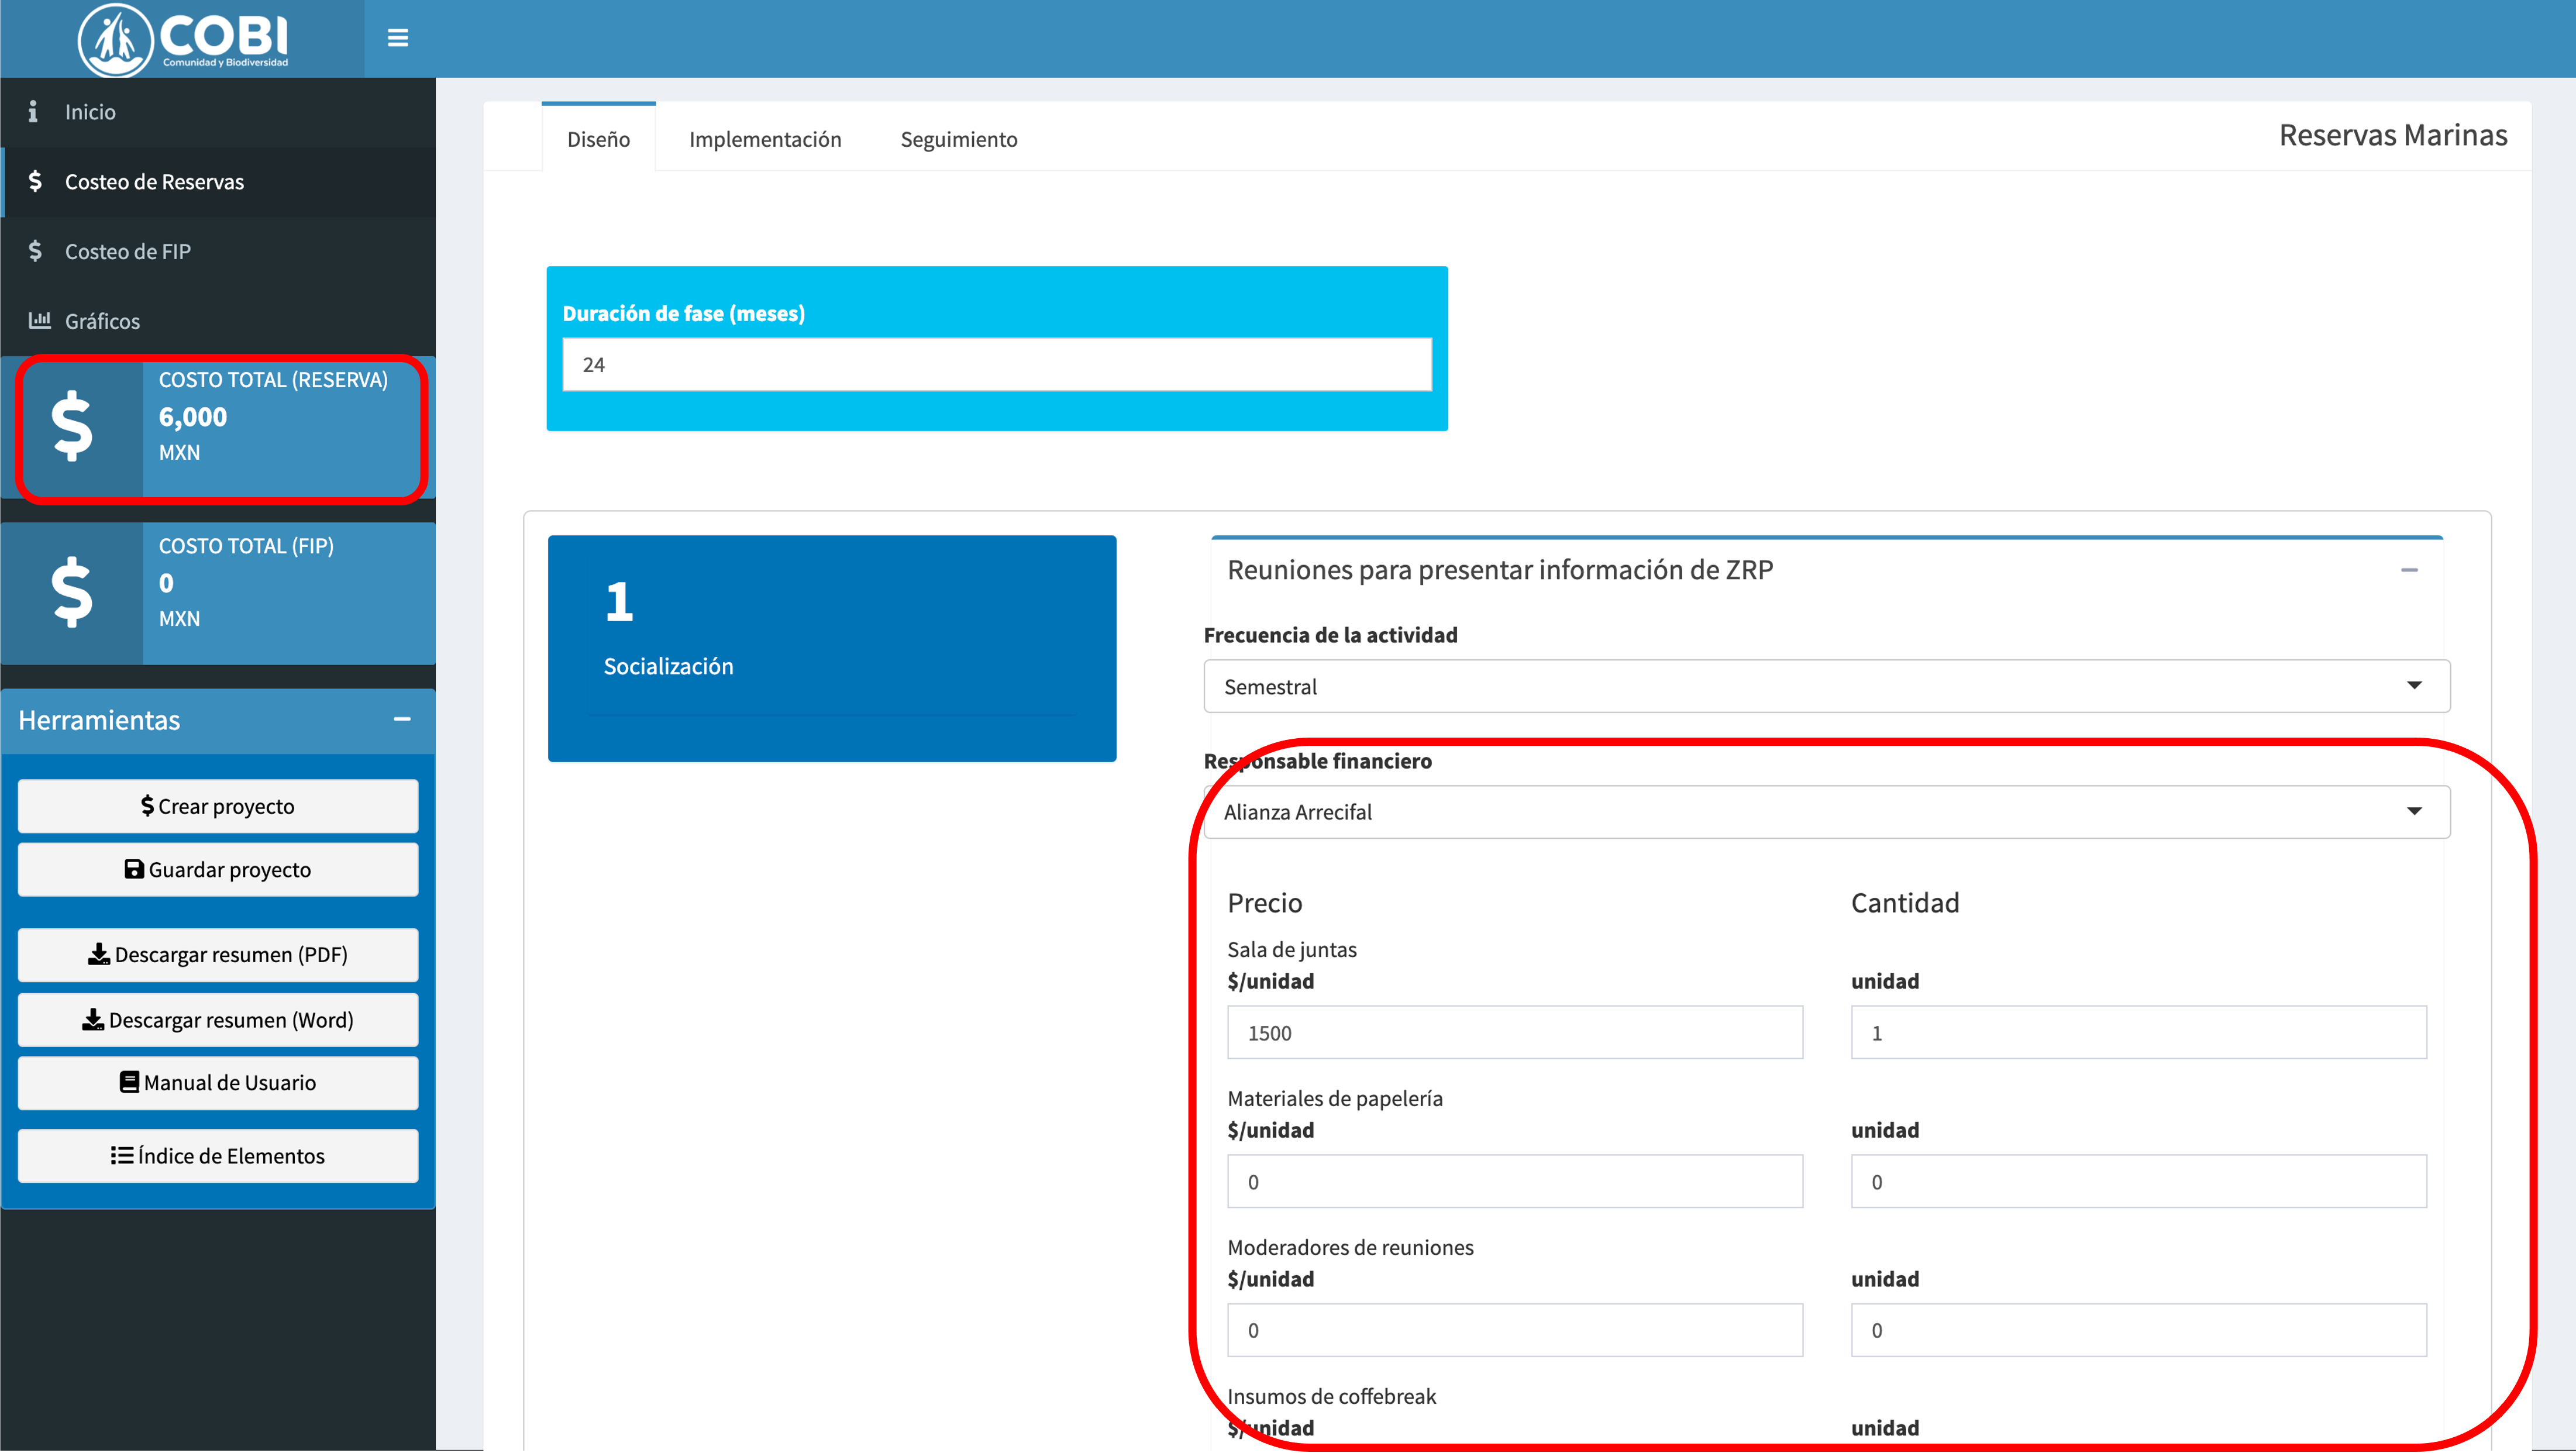
\includegraphics{images/rema_dis_5.png}
\caption{\label{fig:rem-dis-5}Llenado de datos y actualización del presupuesto.}
\end{figure}

\textbf{Paso 6 - } Continua llenando los datos de la actividad, incluyendo los costos y cantidades de todos los elementos relevantes (Fig \ref{fig:rem-dis-6}). En este caso, necesitaremos \$200 en materiales de papelería y 2 moderadores que cobrarán \$3,000 por reunión cada uno. También incluimos los insumos de coffee break, estimados en \$500 por reunión.

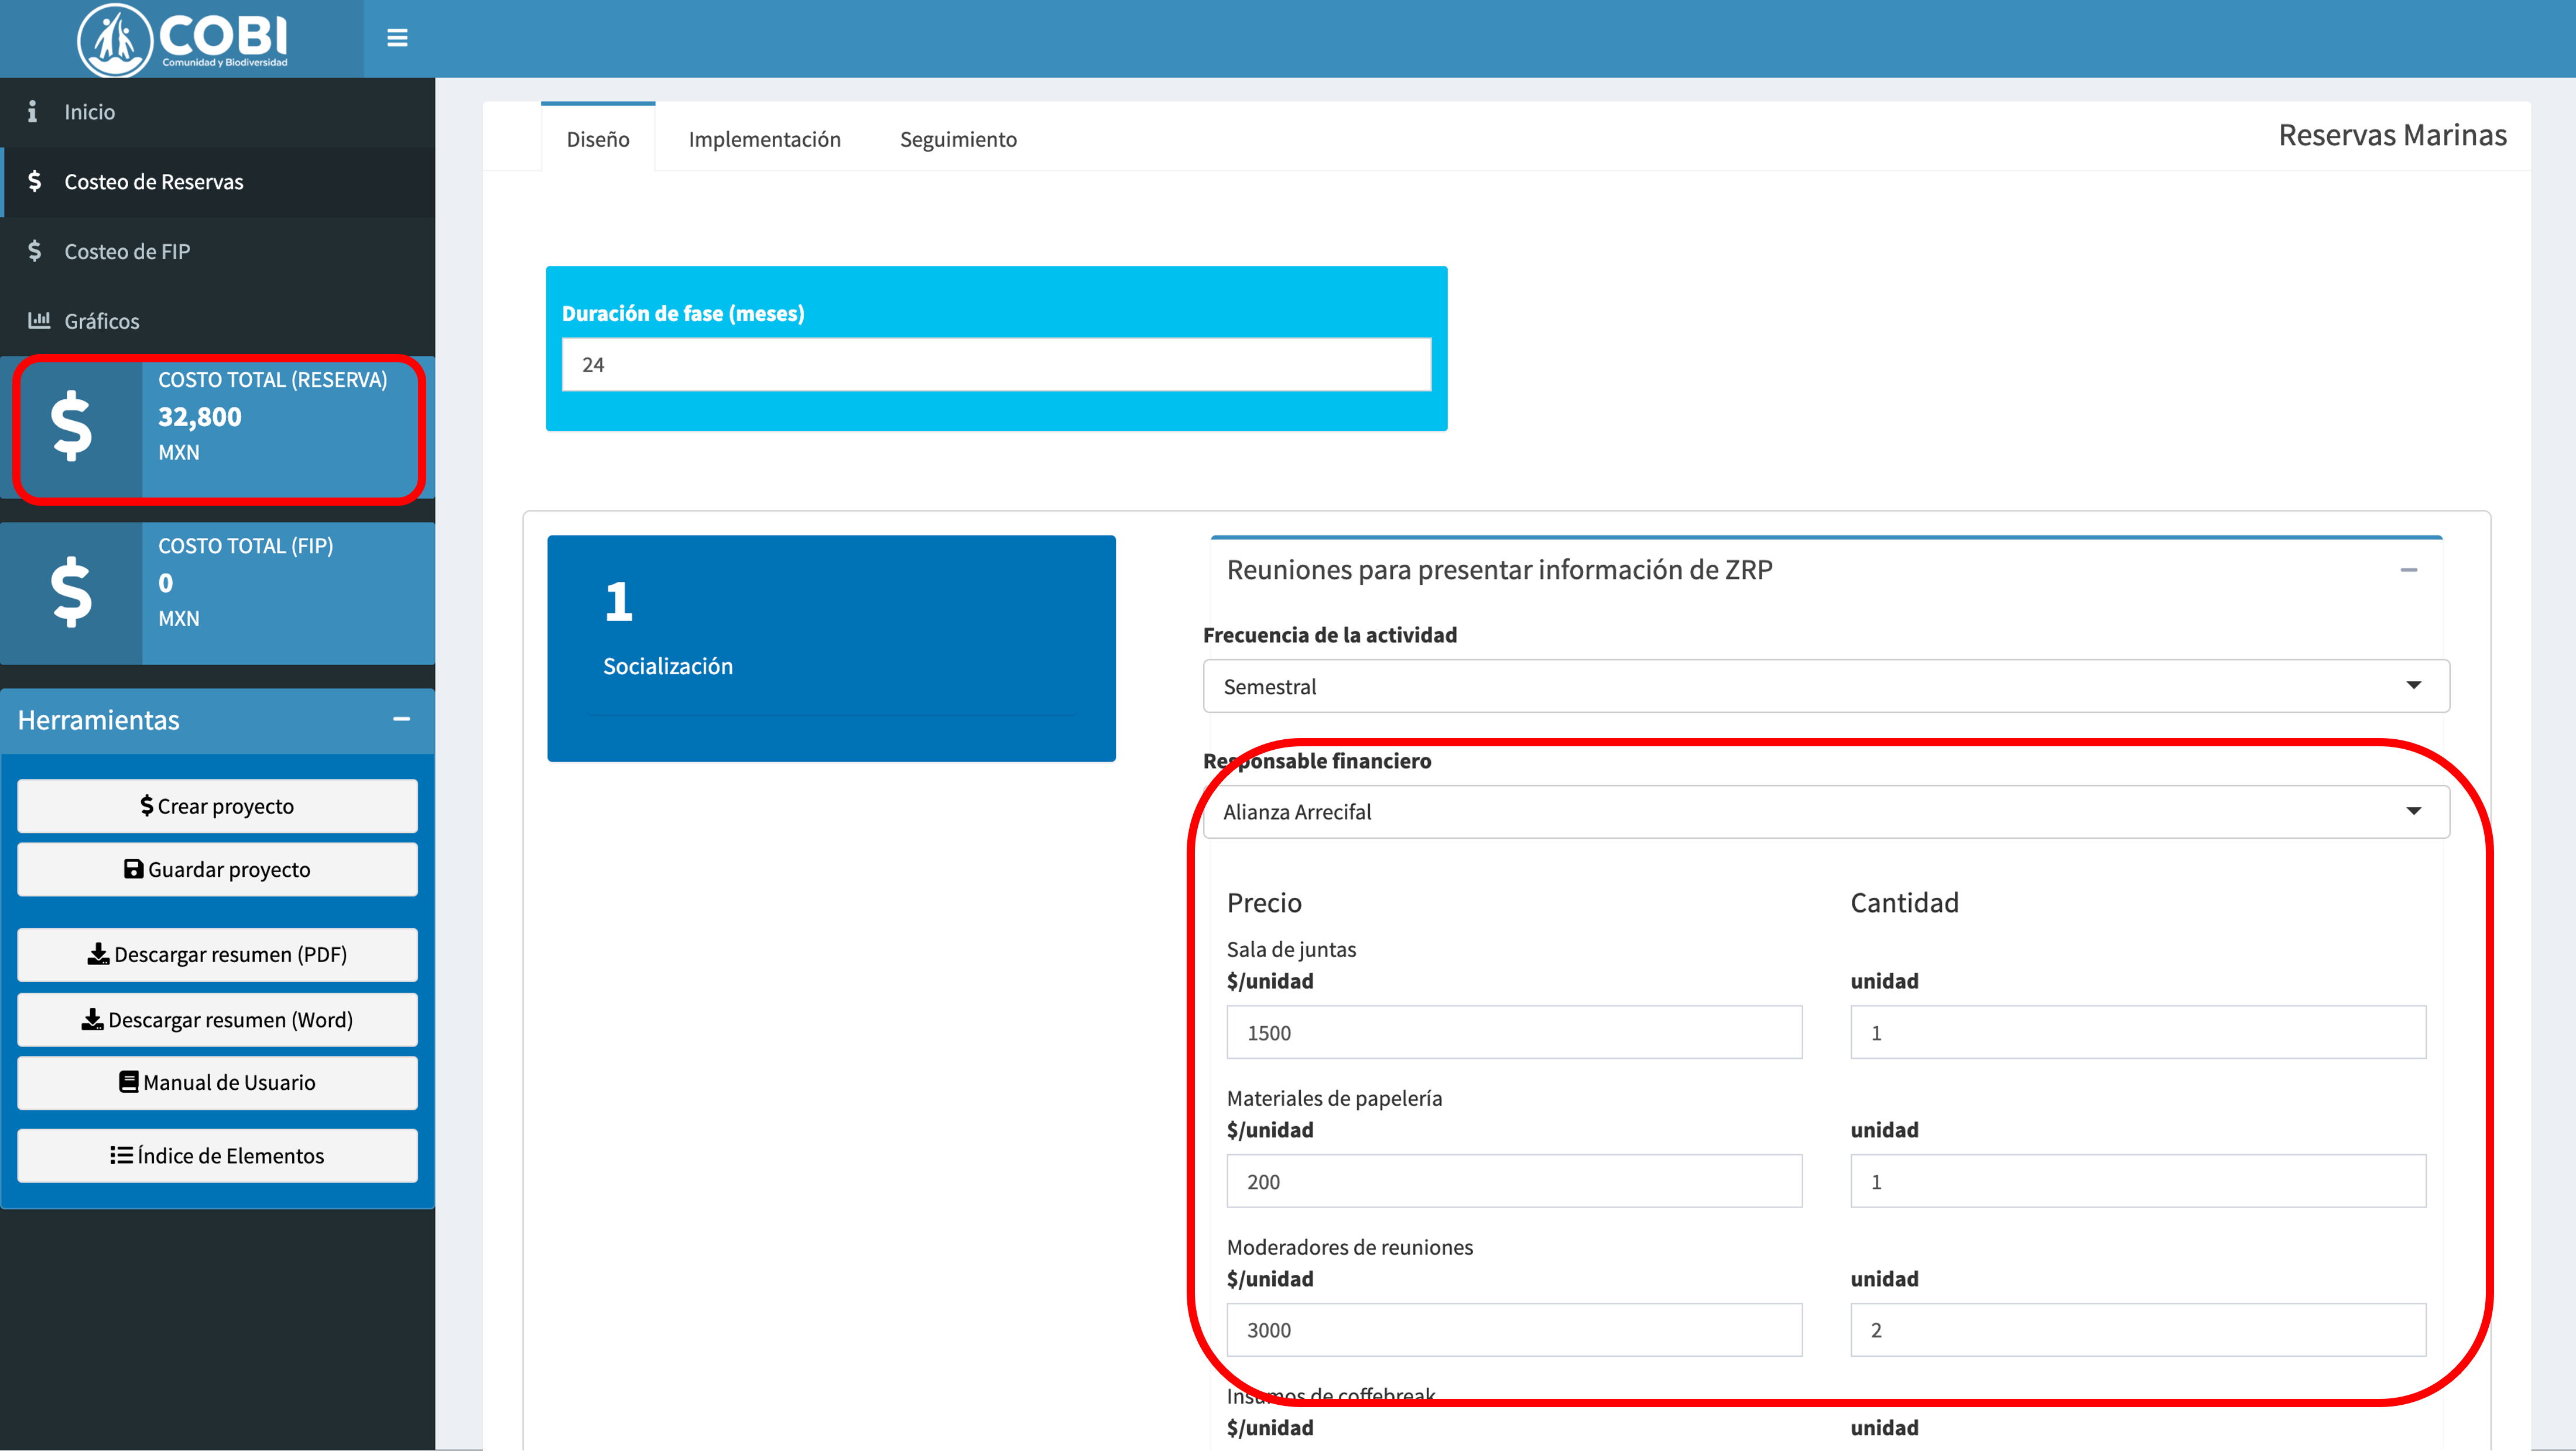
\includegraphics{images/rema_dis_6.png}
\textbf{Paso 7 - } Una vez hayas terminado con la actividad, ha click en el signo \textbf{-} para colapsar el formato de entrada y repite los pasos 3 - 6 para llenar las siguientes actividades (Fig \ref{fig:rem-dis-7}). Observa cómo la actividad de reuniones está colapsada, mientras que la actividad de reunión para definir objetivos ahora está disponible.

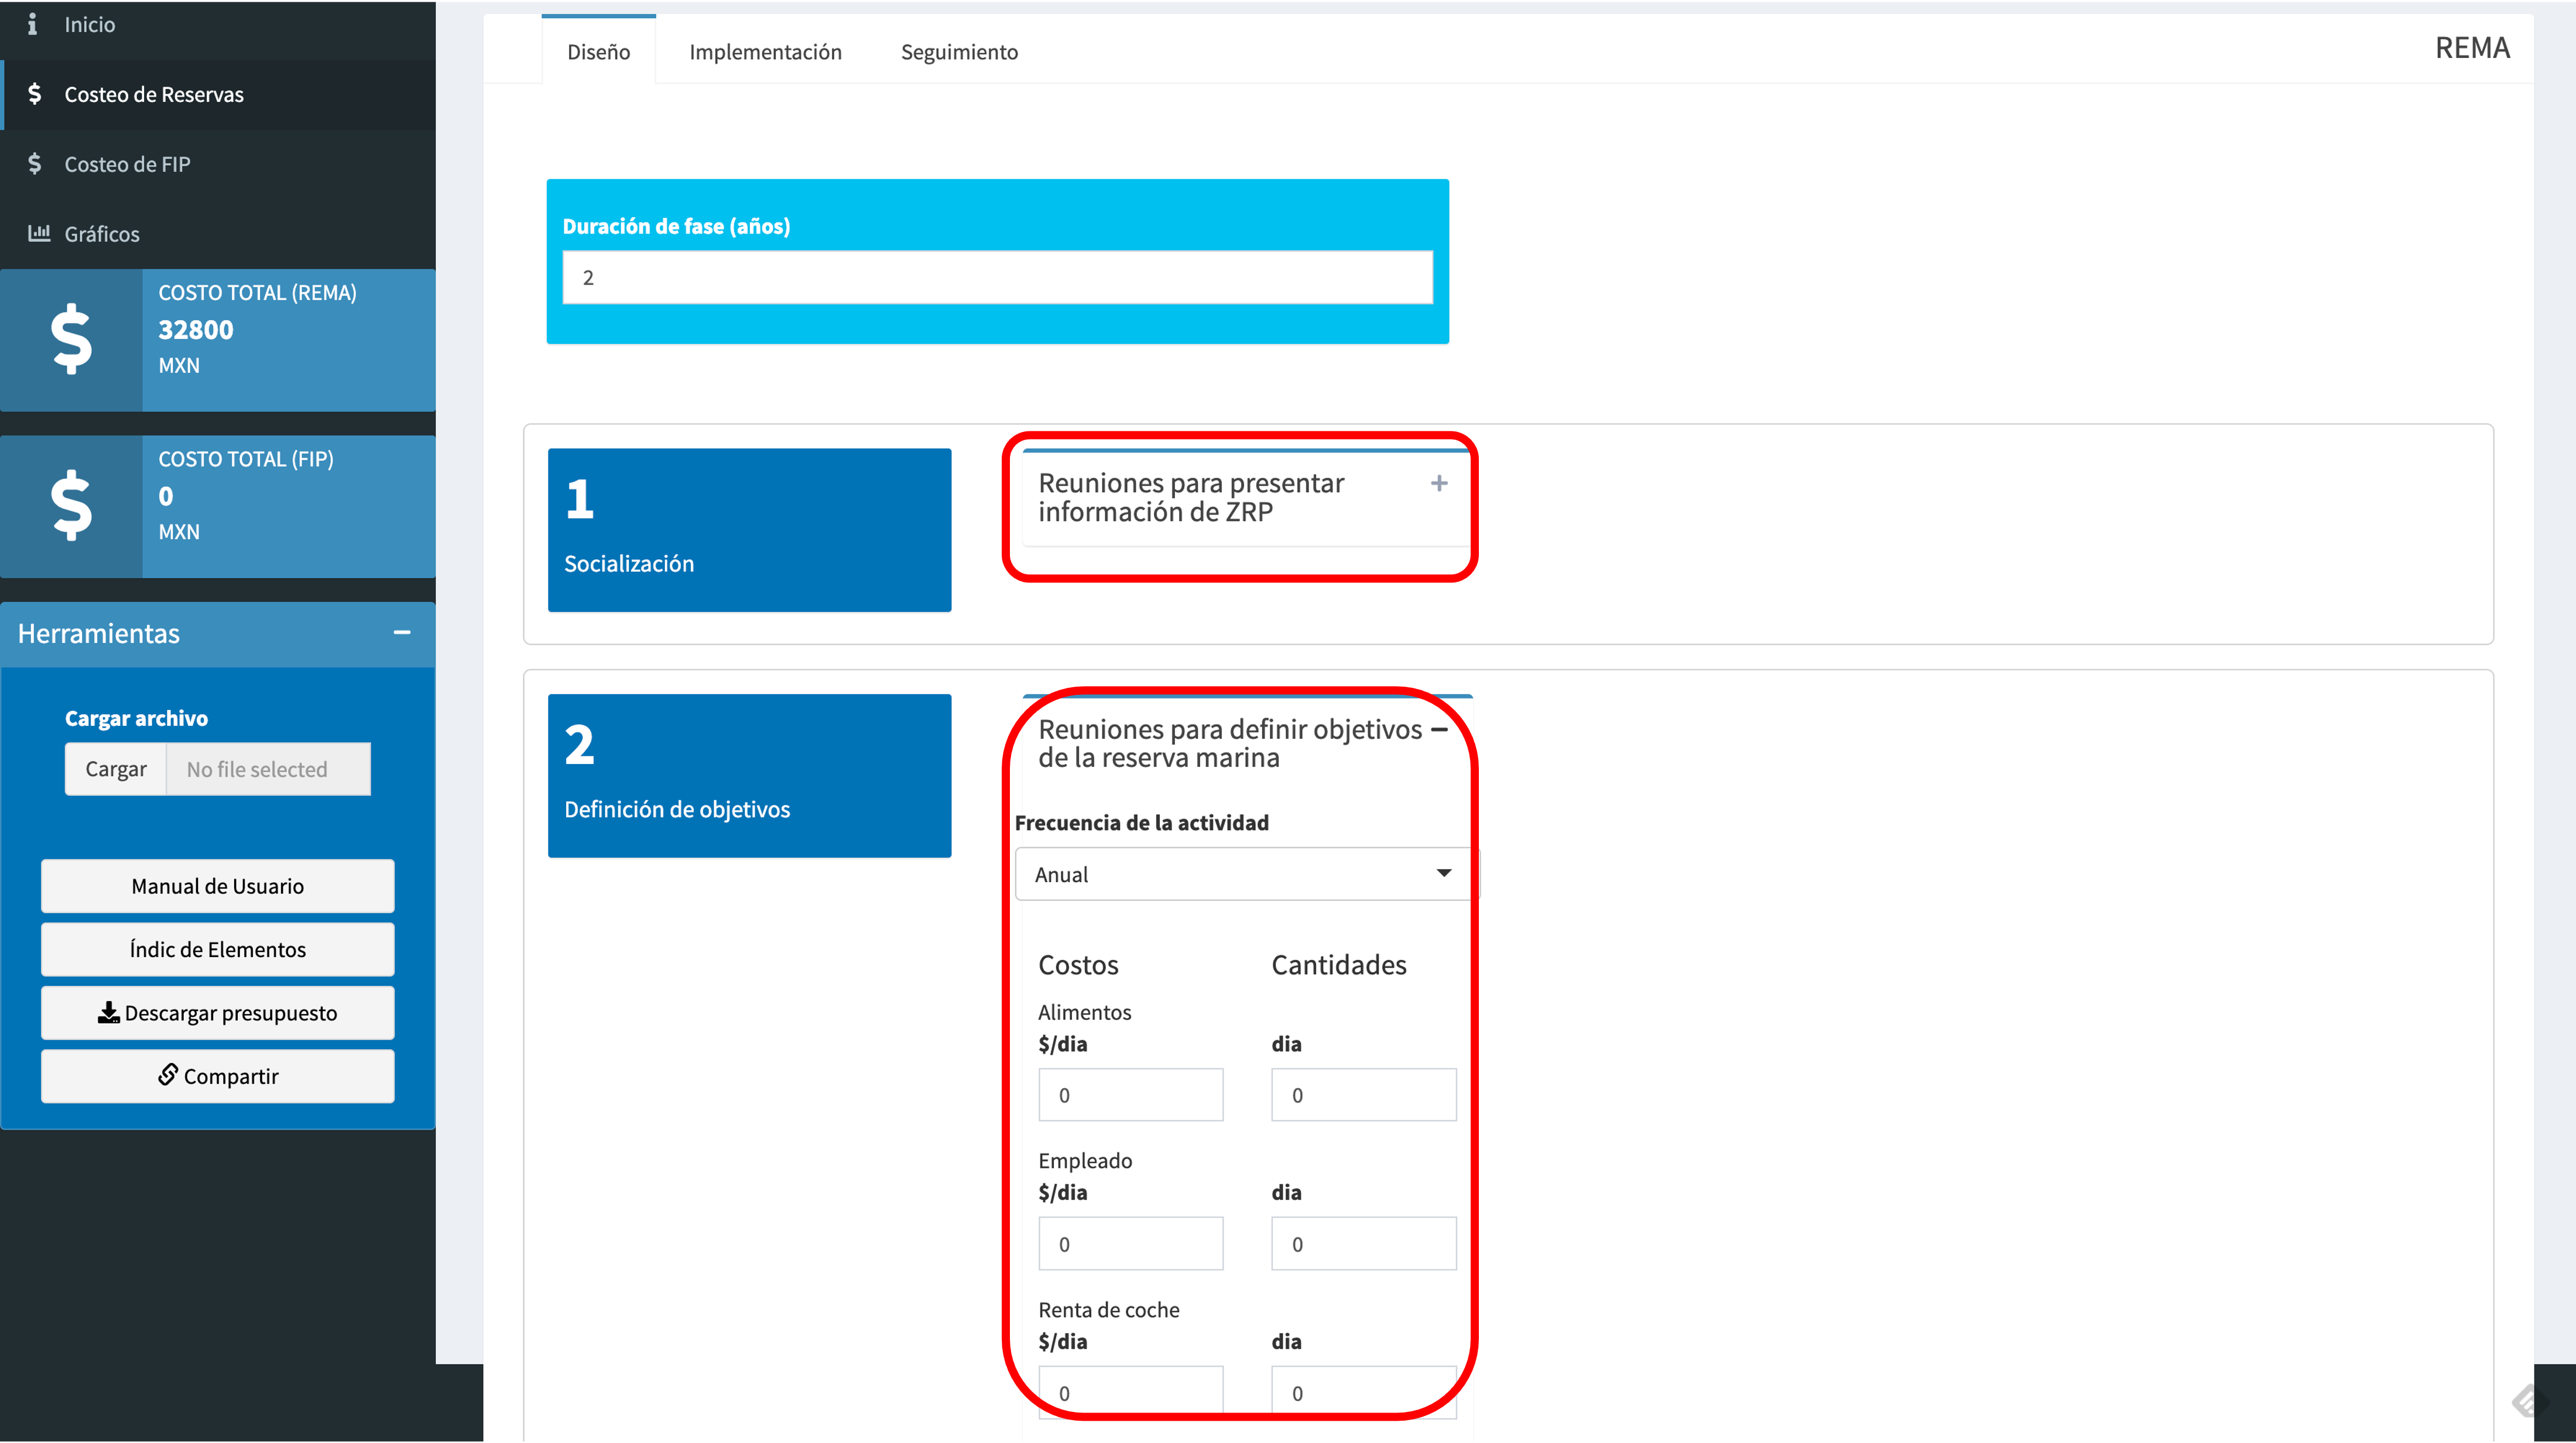
\includegraphics{images/rema_dis_7.png}

Esto concluye la breve introducción para el llenado de un presupuesto para REMA. En un ejercicio real, probablemente necesites iterar más entre fases, subfases y actividades. En cualquier momento puedes navegar a otras secciones, por ejemplo para explorar y visualizar el presupuesto, descrito a detalle en el capítulo \ref{explorar}.

\hypertarget{fip}{%
\section{Ejemplo de FIP}\label{fip}}

Supongamos que ya haz cubierto la fase de diseño para un FIP. El siguiente pso es la fase de implementación, donde se selecciona y plana el tipo de intervenciones.

\textbf{Paso 1 - } Selecciona la sección de ``Costeo de FIP'' en la barra lateral (Fig \ref{fig:fip-imp-1}).

\begin{figure}
\centering
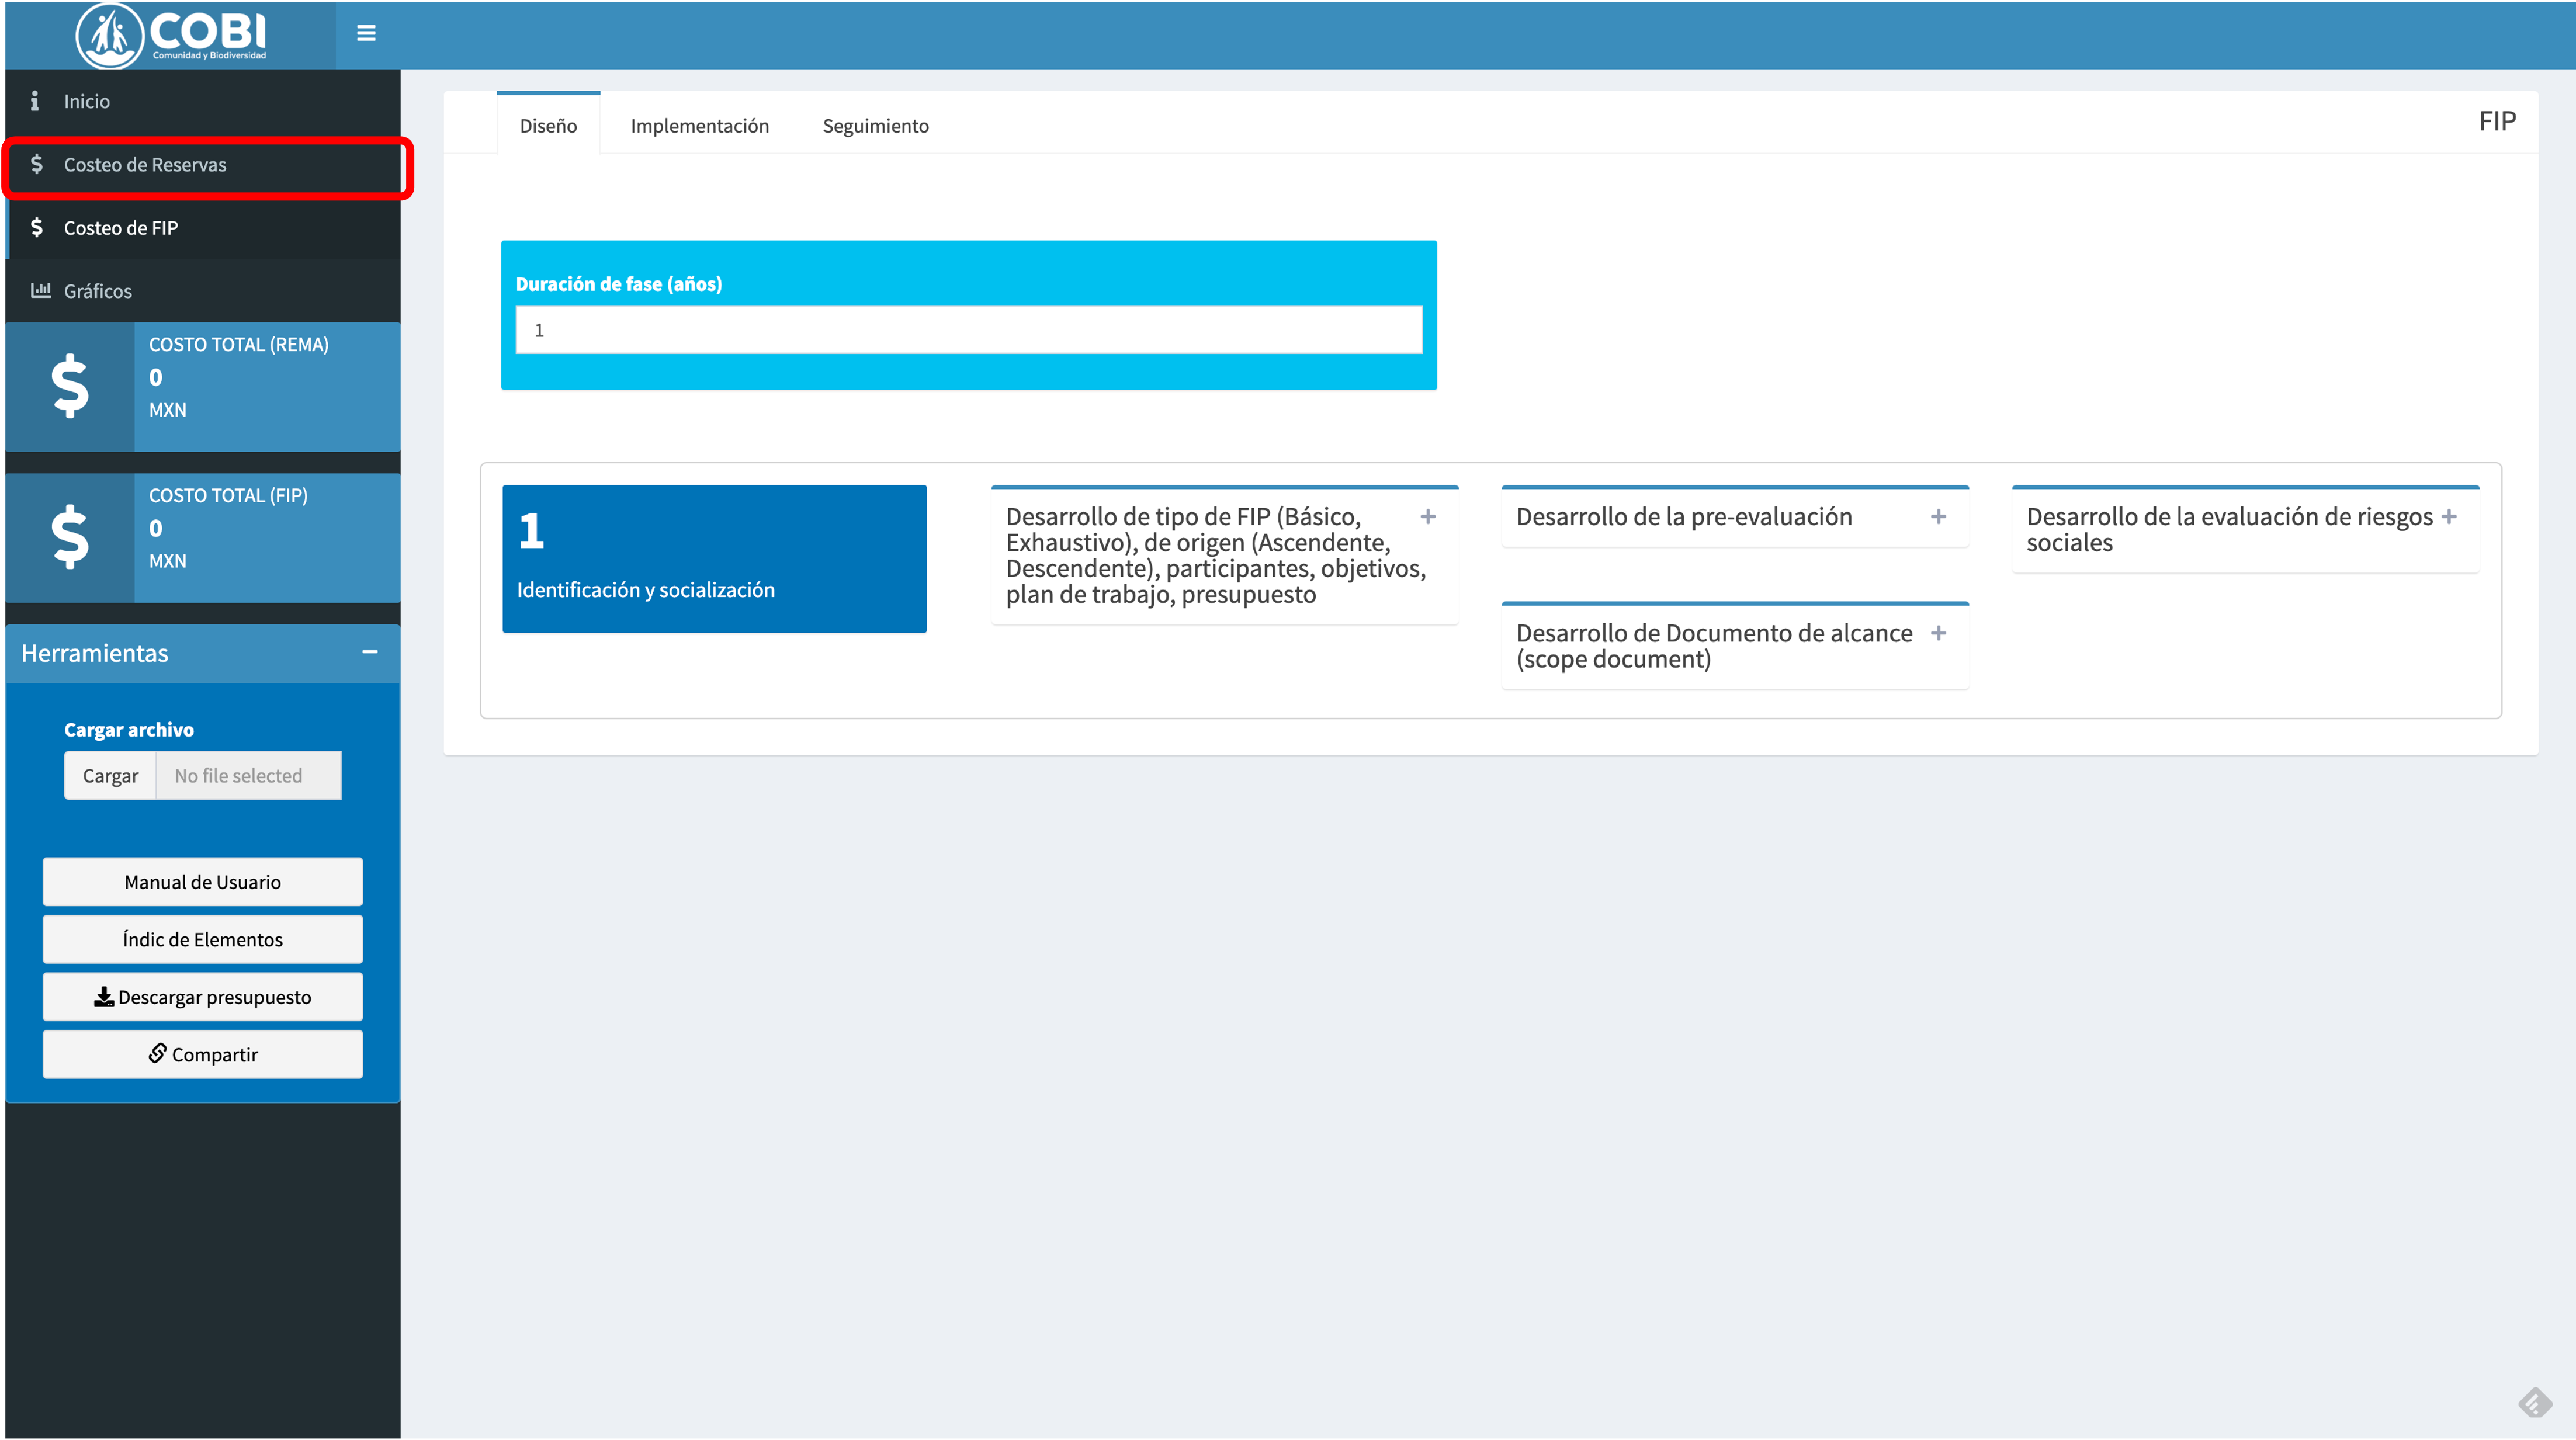
\includegraphics{images/fip-imp-1.png}
\caption{\label{fig:fip-imp-1}Selecciona la sección.}
\end{figure}

\textbf{Paso 2 - } En el área de trabajo de FIP, selecciona la pestaña de ``Implementación'' en la parte superior de la pantalla. (Fig \ref{fig:fip-imp-2}).

\begin{figure}
\centering
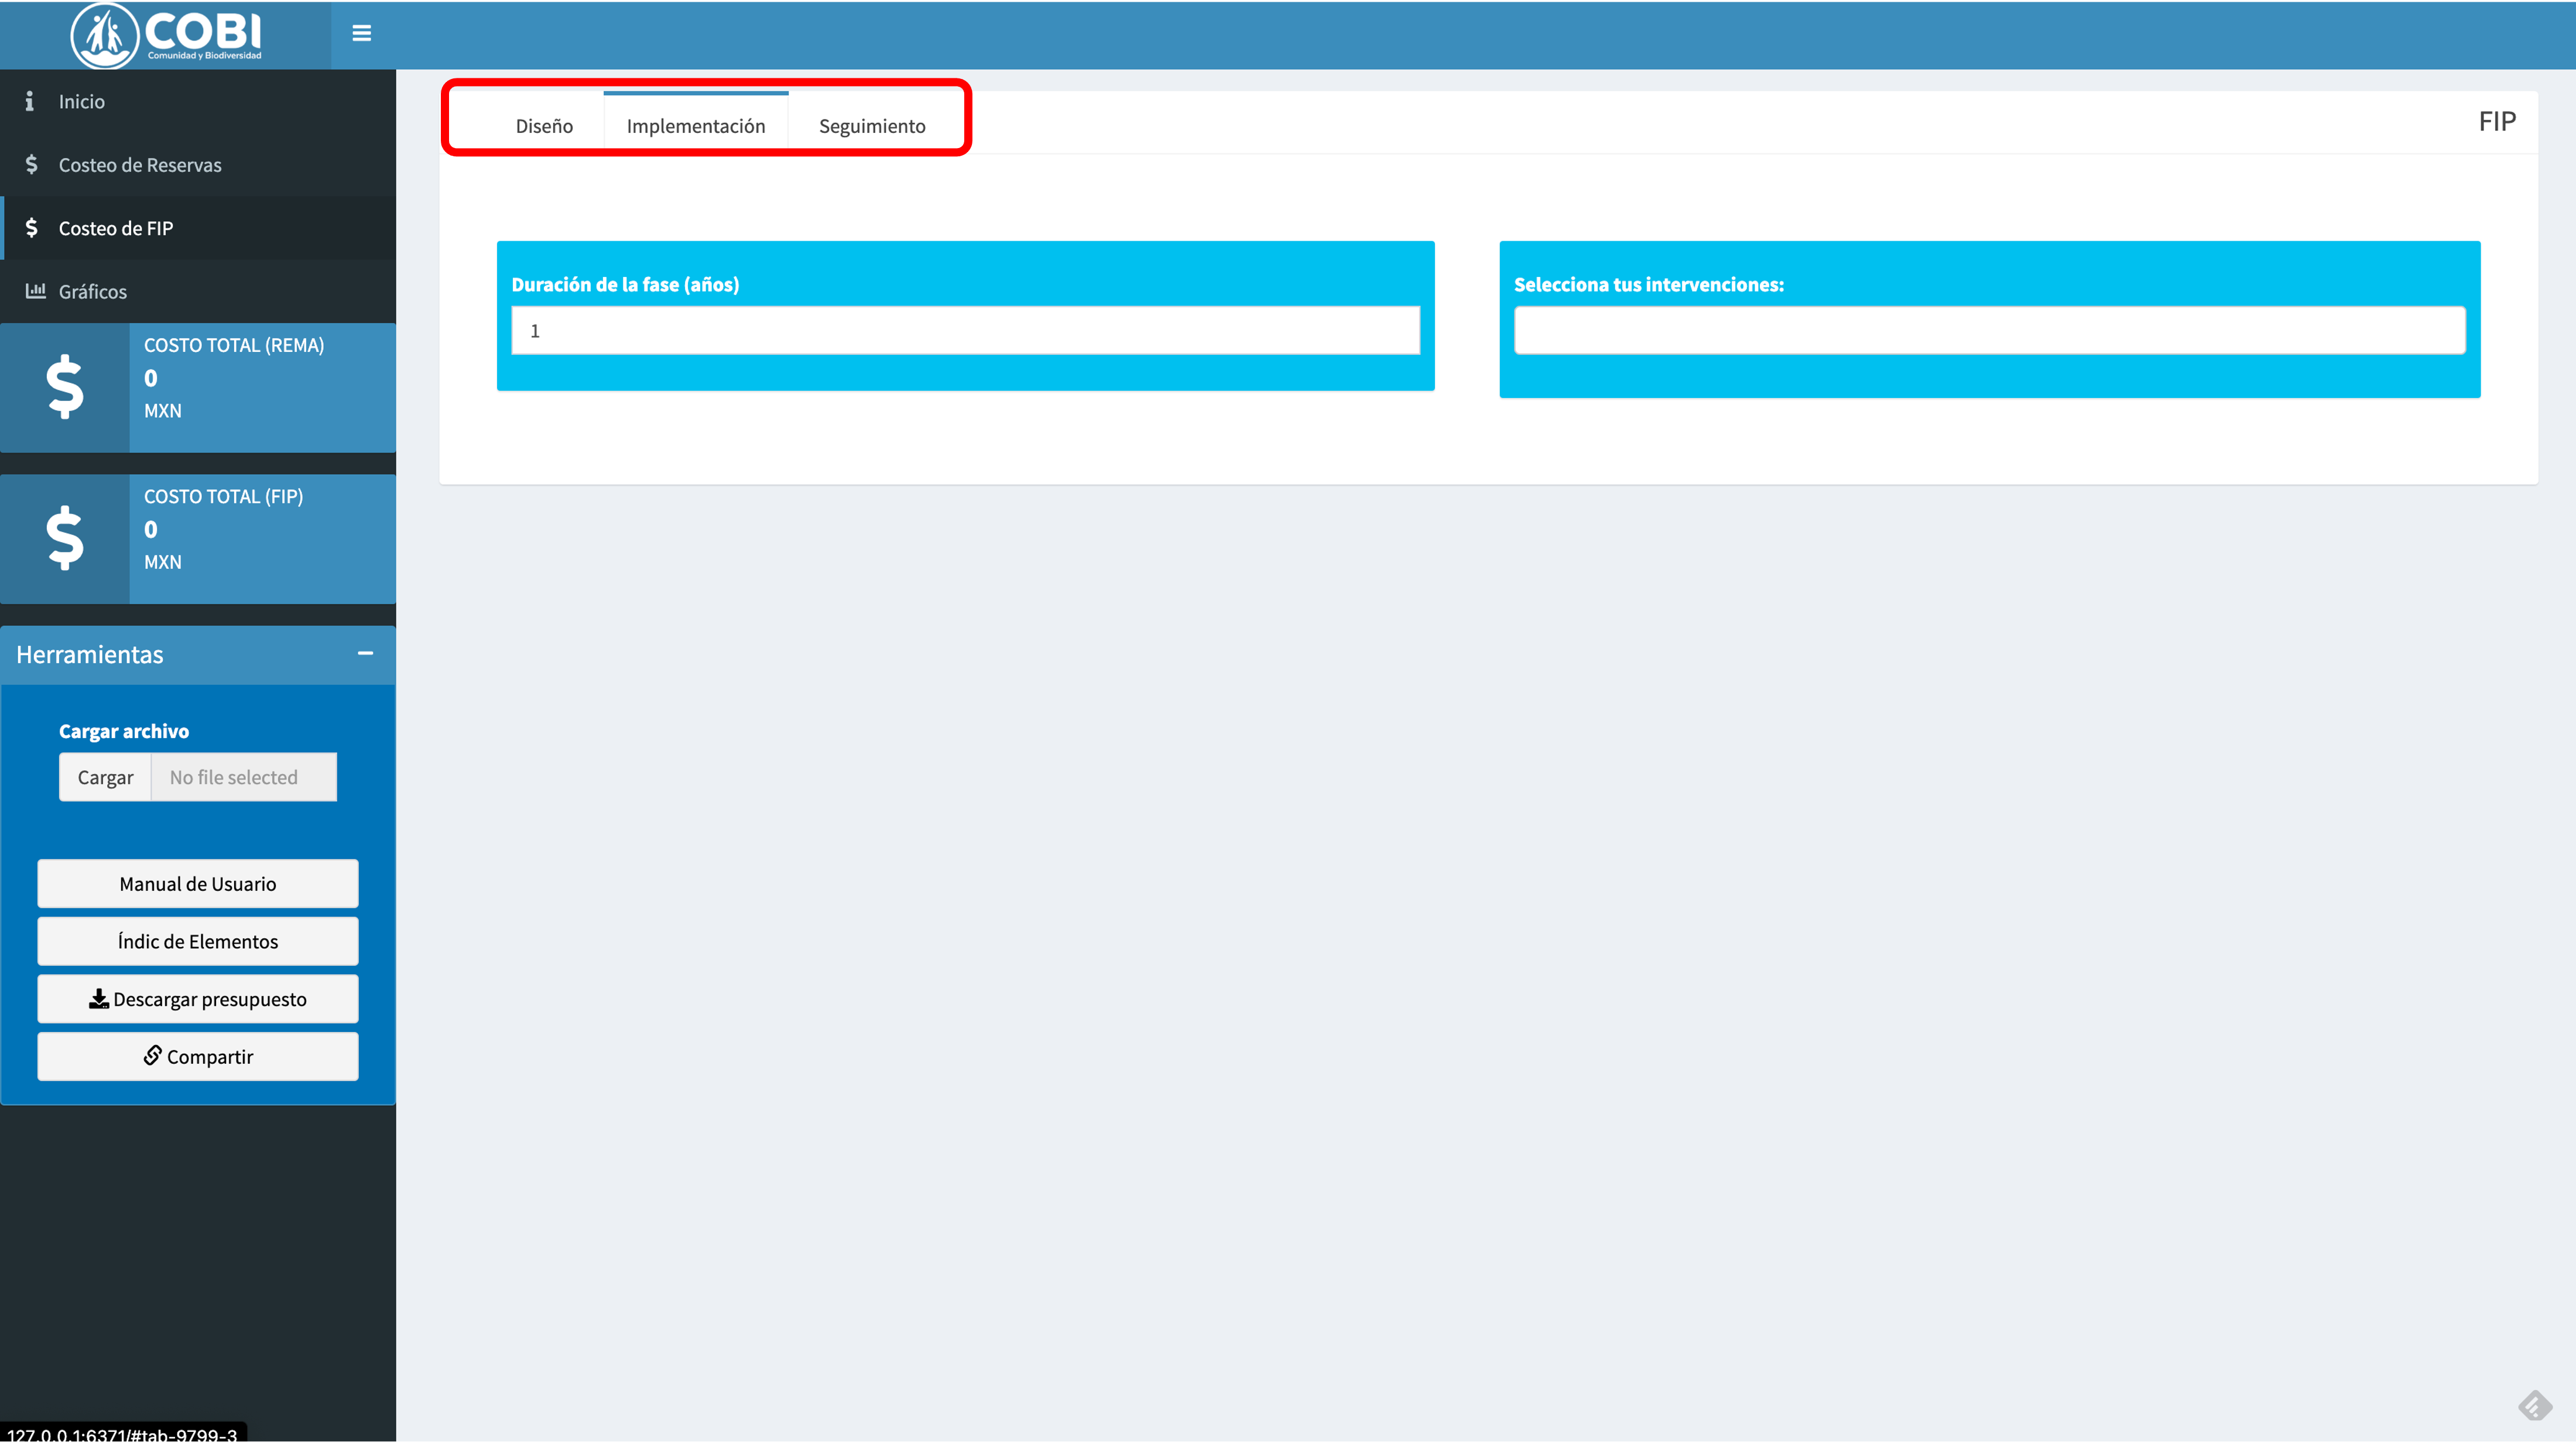
\includegraphics{images/fip-imp-2.png}
\caption{\label{fig:fip-imp-2}Selecciona la fase}
\end{figure}

\textbf{Paso 2 - } Ingresa la duración de la fase, en este caso de 2 años (Fig \ref{fig:fip-imp-3}).

\begin{figure}
\centering
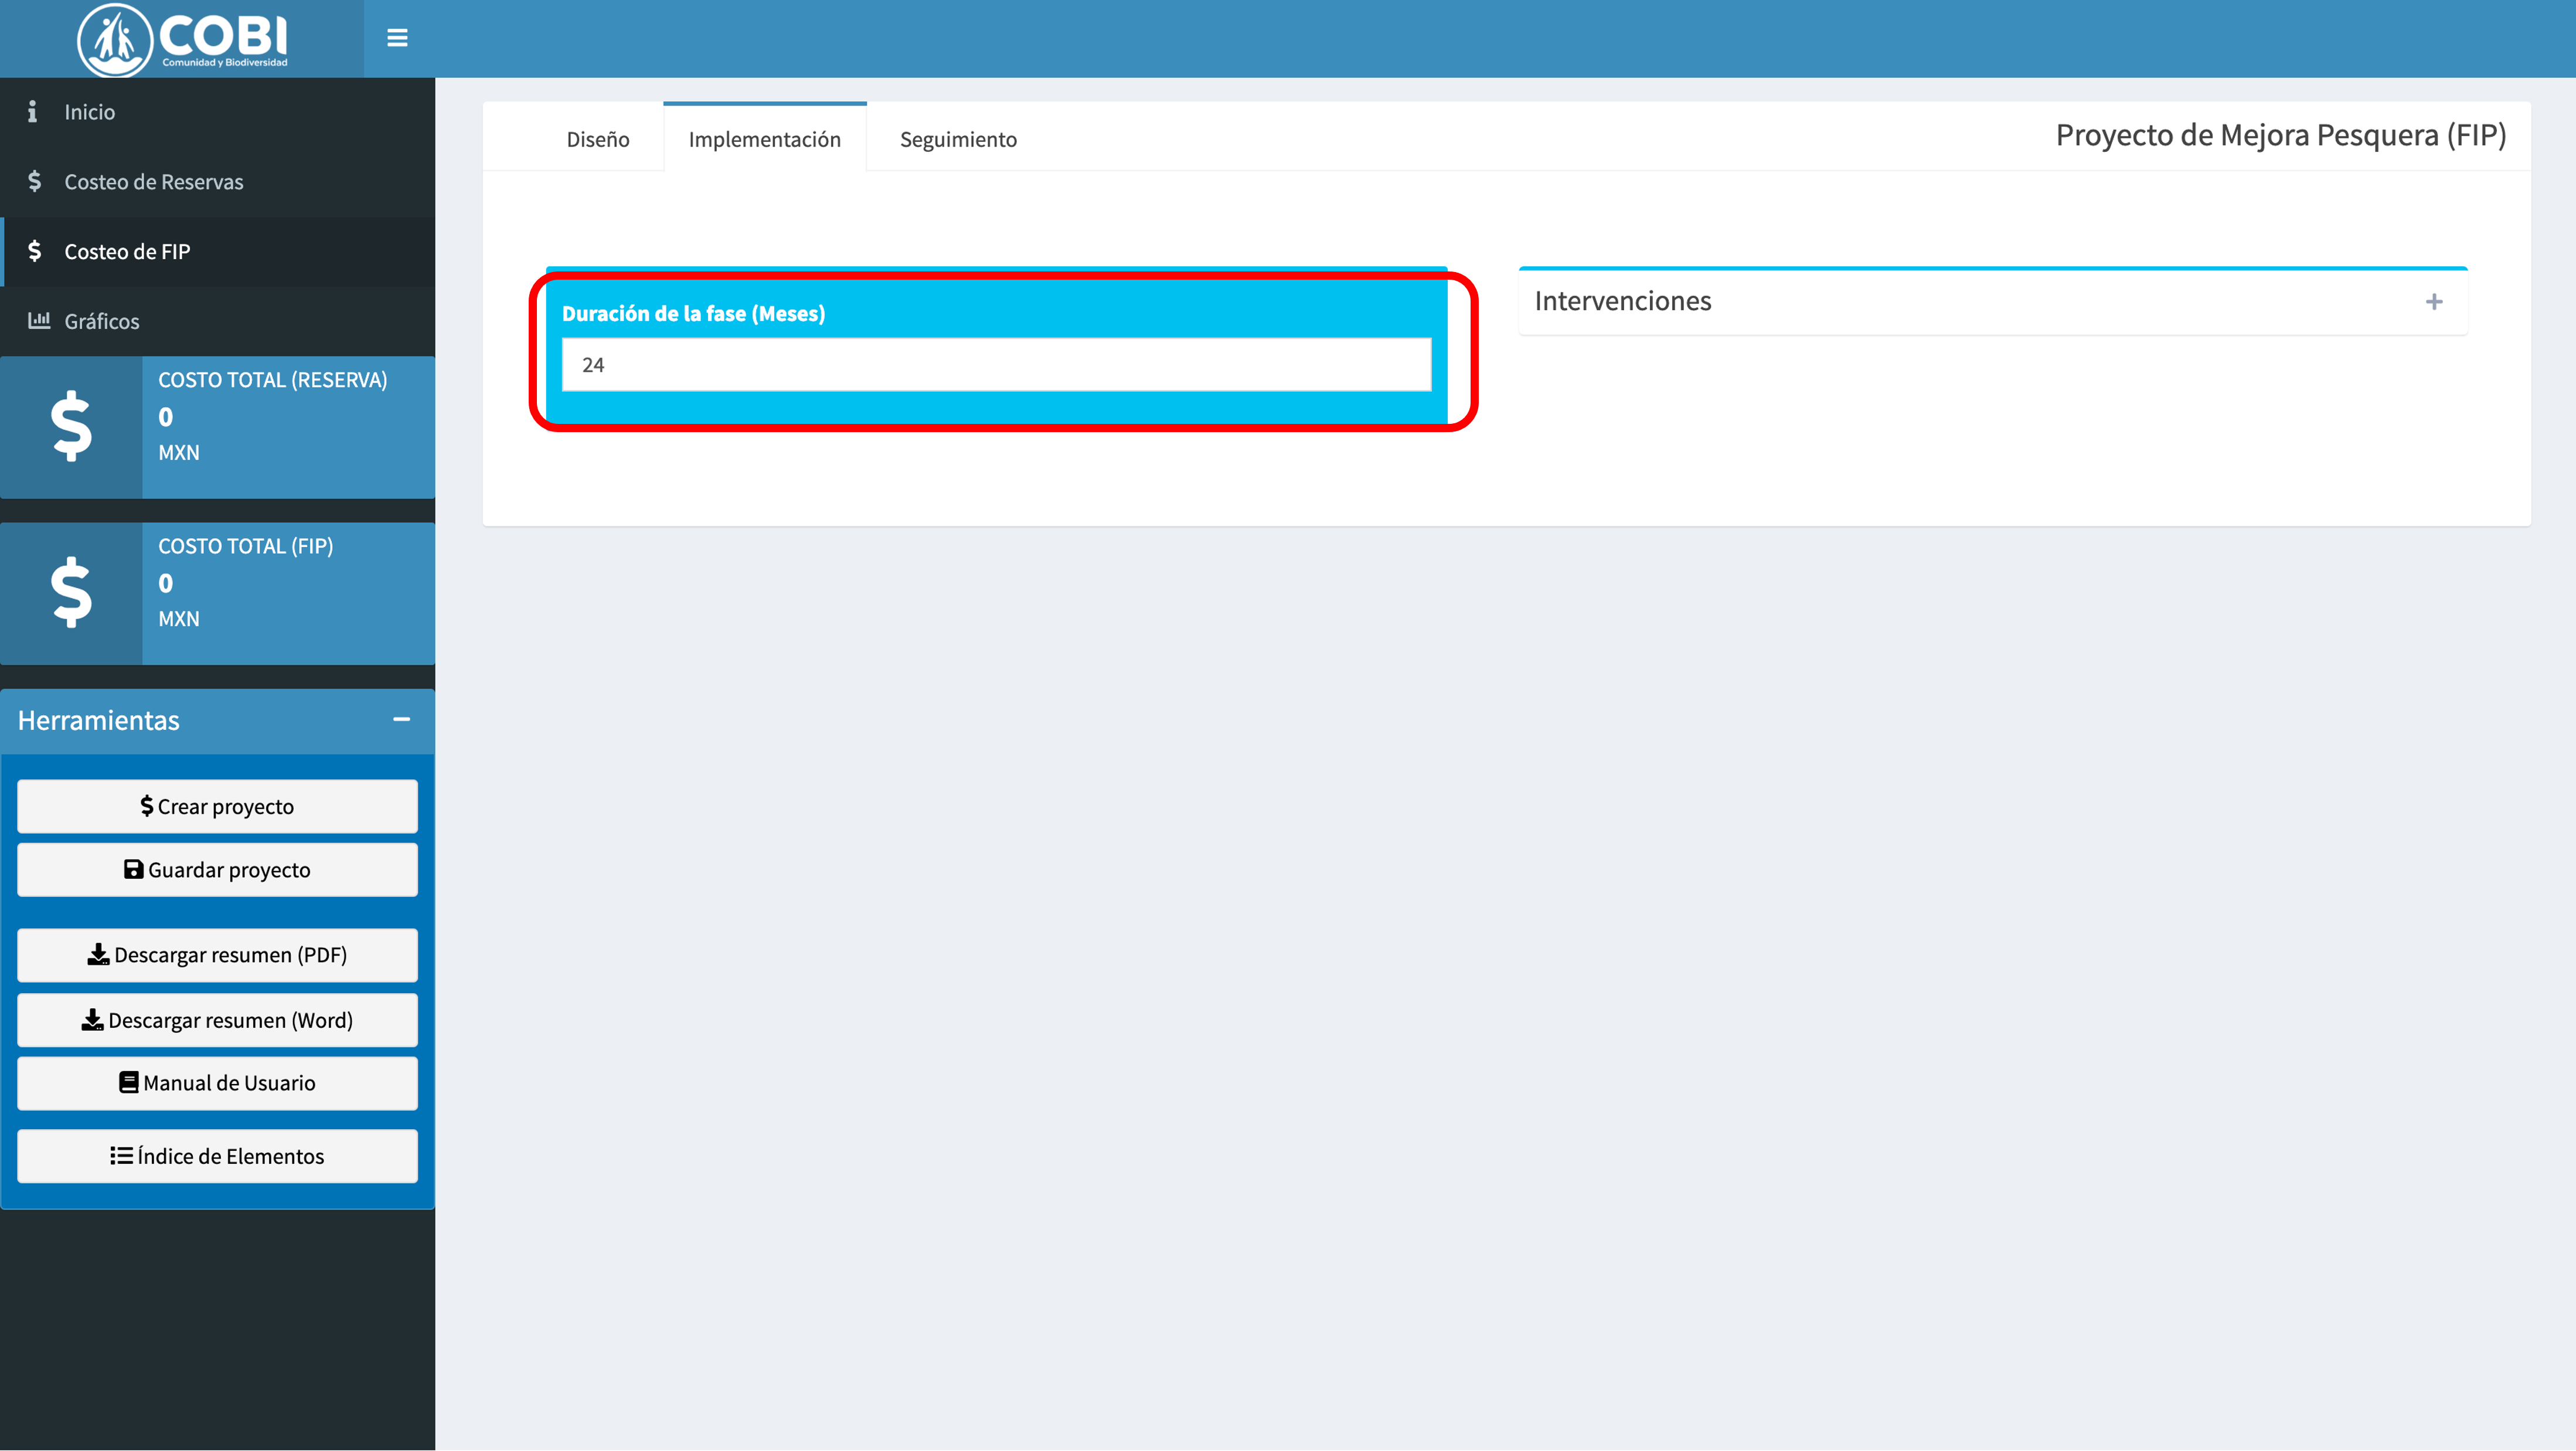
\includegraphics{images/fip-imp-3.png}
\caption{\label{fig:fip-imp-3}Selecciona la duración de la fase.}
\end{figure}

\textbf{Paso 4 - } Un FIP puede tener diferentes intervenciones. Usa el menú desplegable del lado derecho para seleccionar las intervenciones que corresponden a tu programa (Fig \ref{fig:fip-imp-4}).

\begin{figure}
\centering
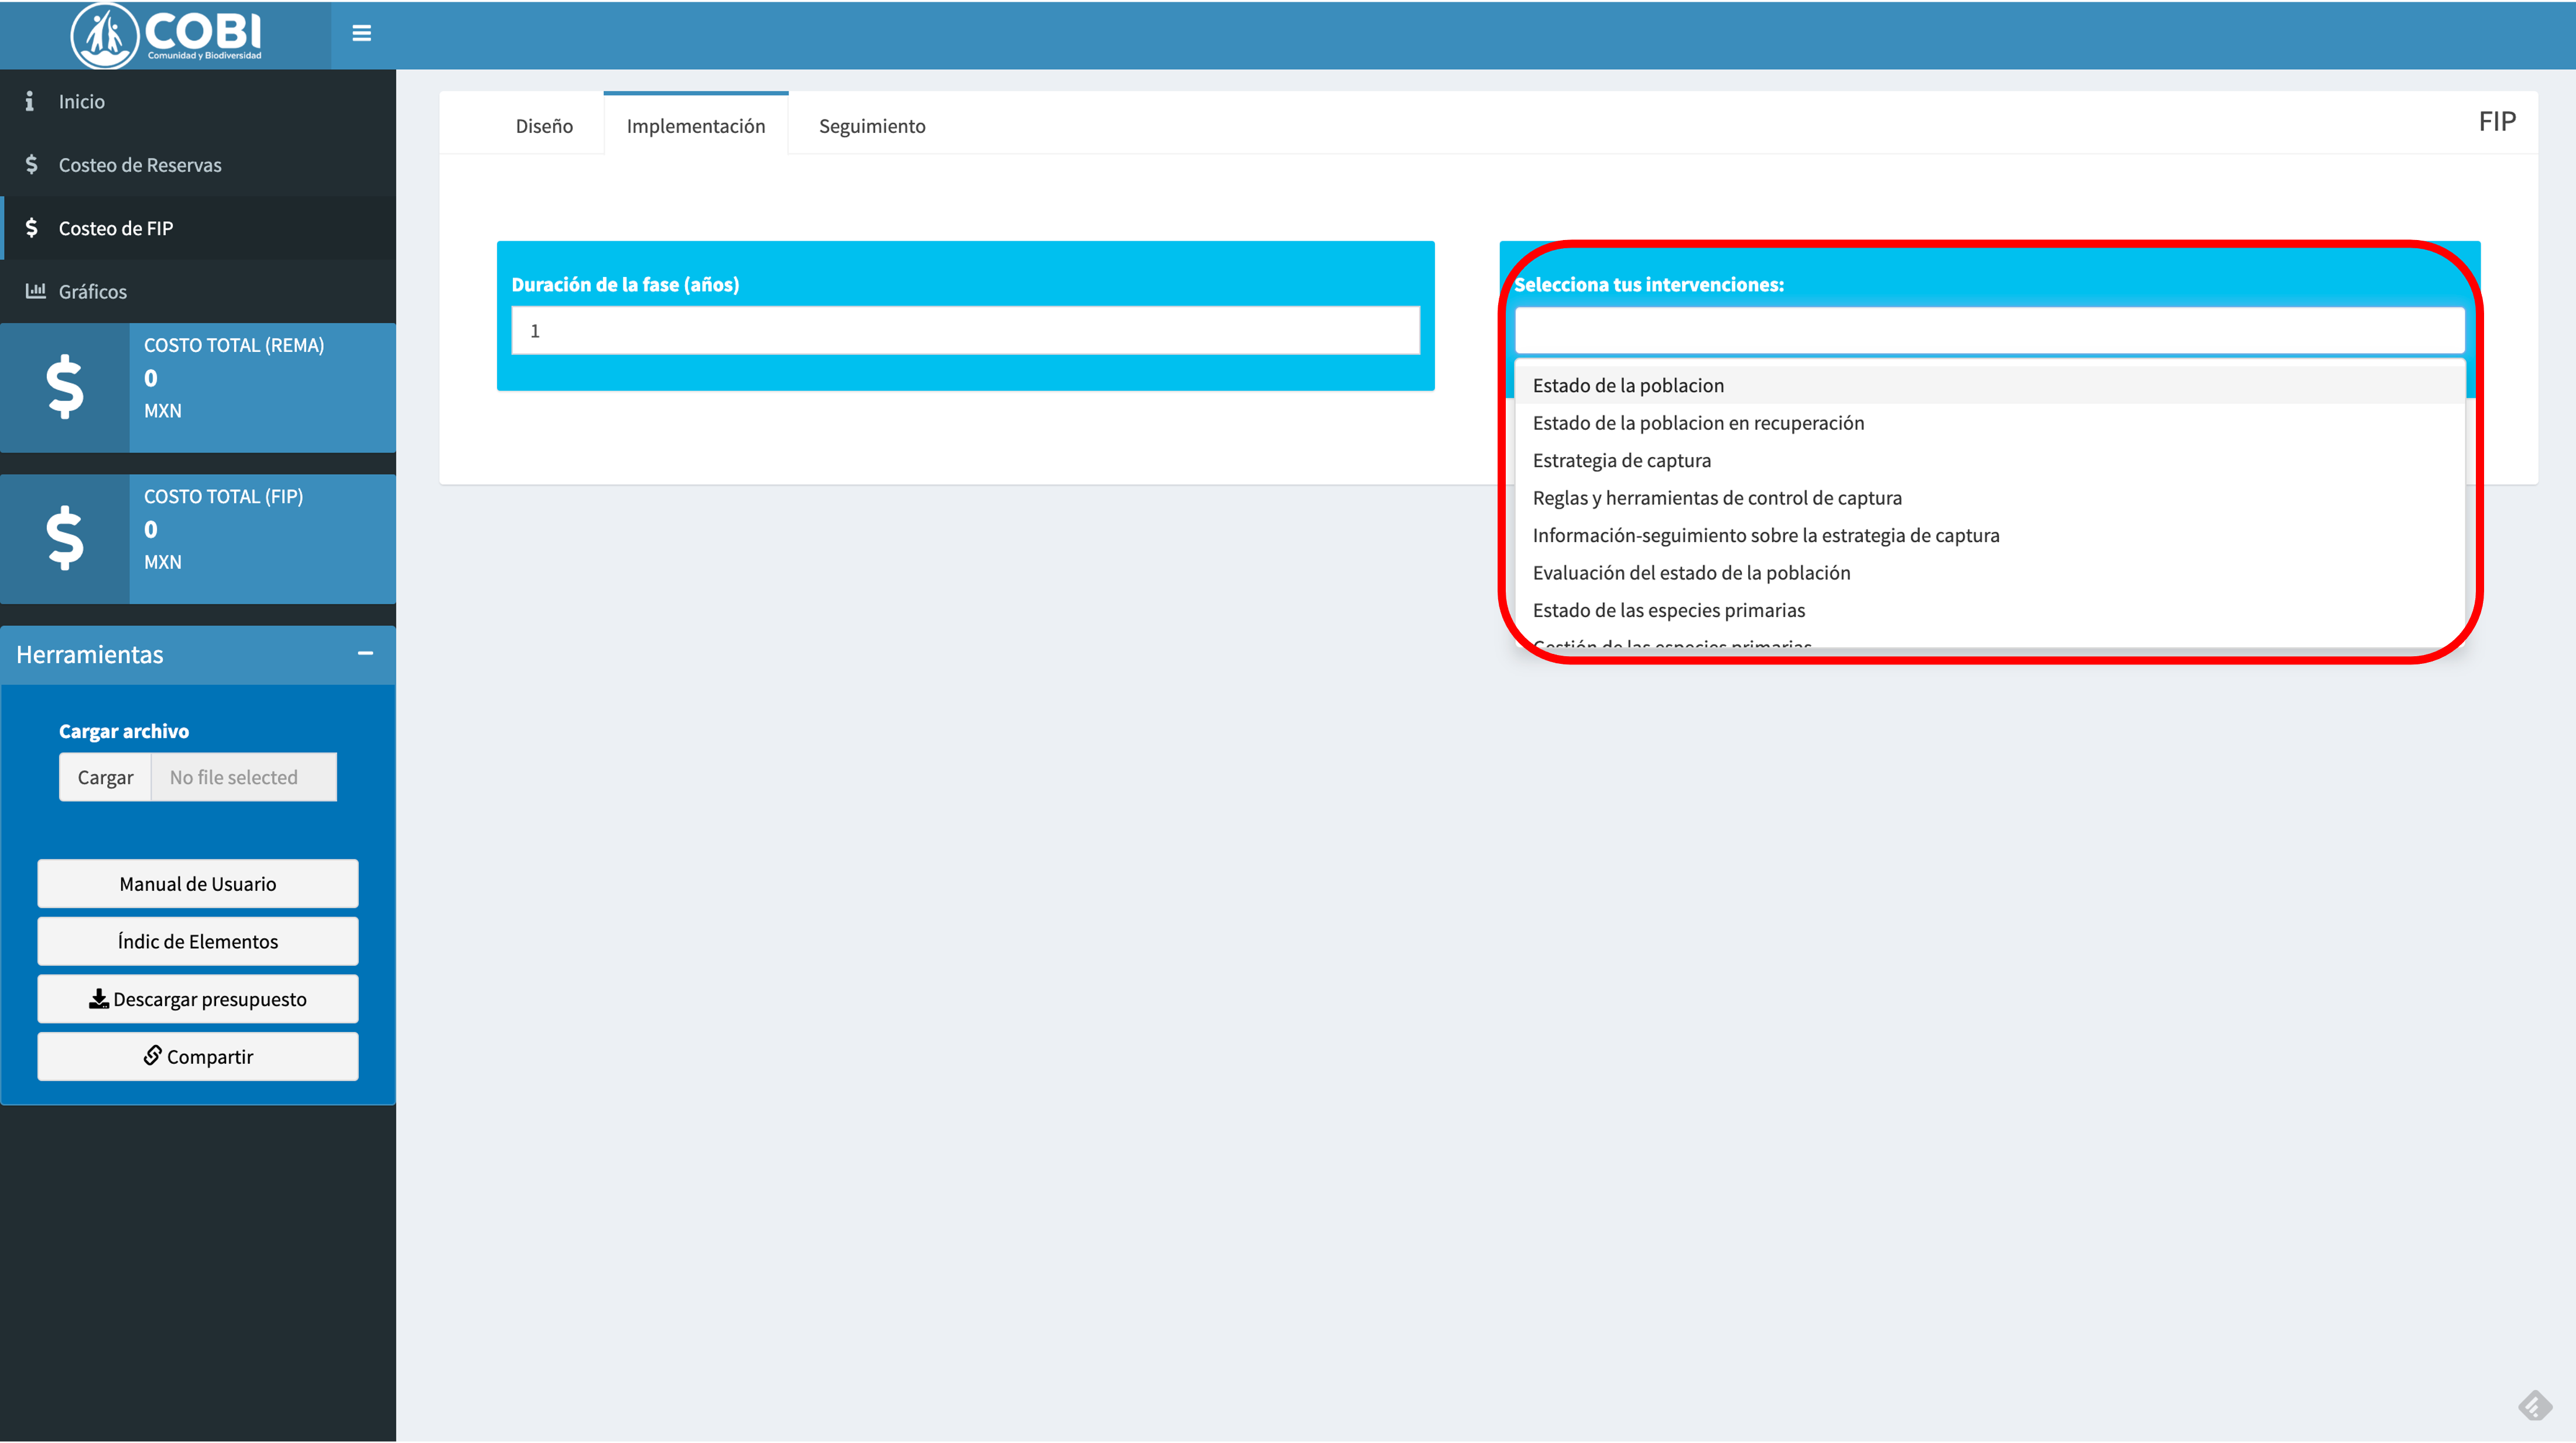
\includegraphics{images/fip-imp-4.png}
\caption{\label{fig:fip-imp-4}Selecciona tus acciones.}
\end{figure}

\textbf{Paso 5 - } Al seleccionar las acciones de intervención, el área de trabajo automáticamente generará una subfase para cada una, con las actividades correspondientes (Fig \ref{fig:fip-imp-5}).

\begin{figure}
\centering
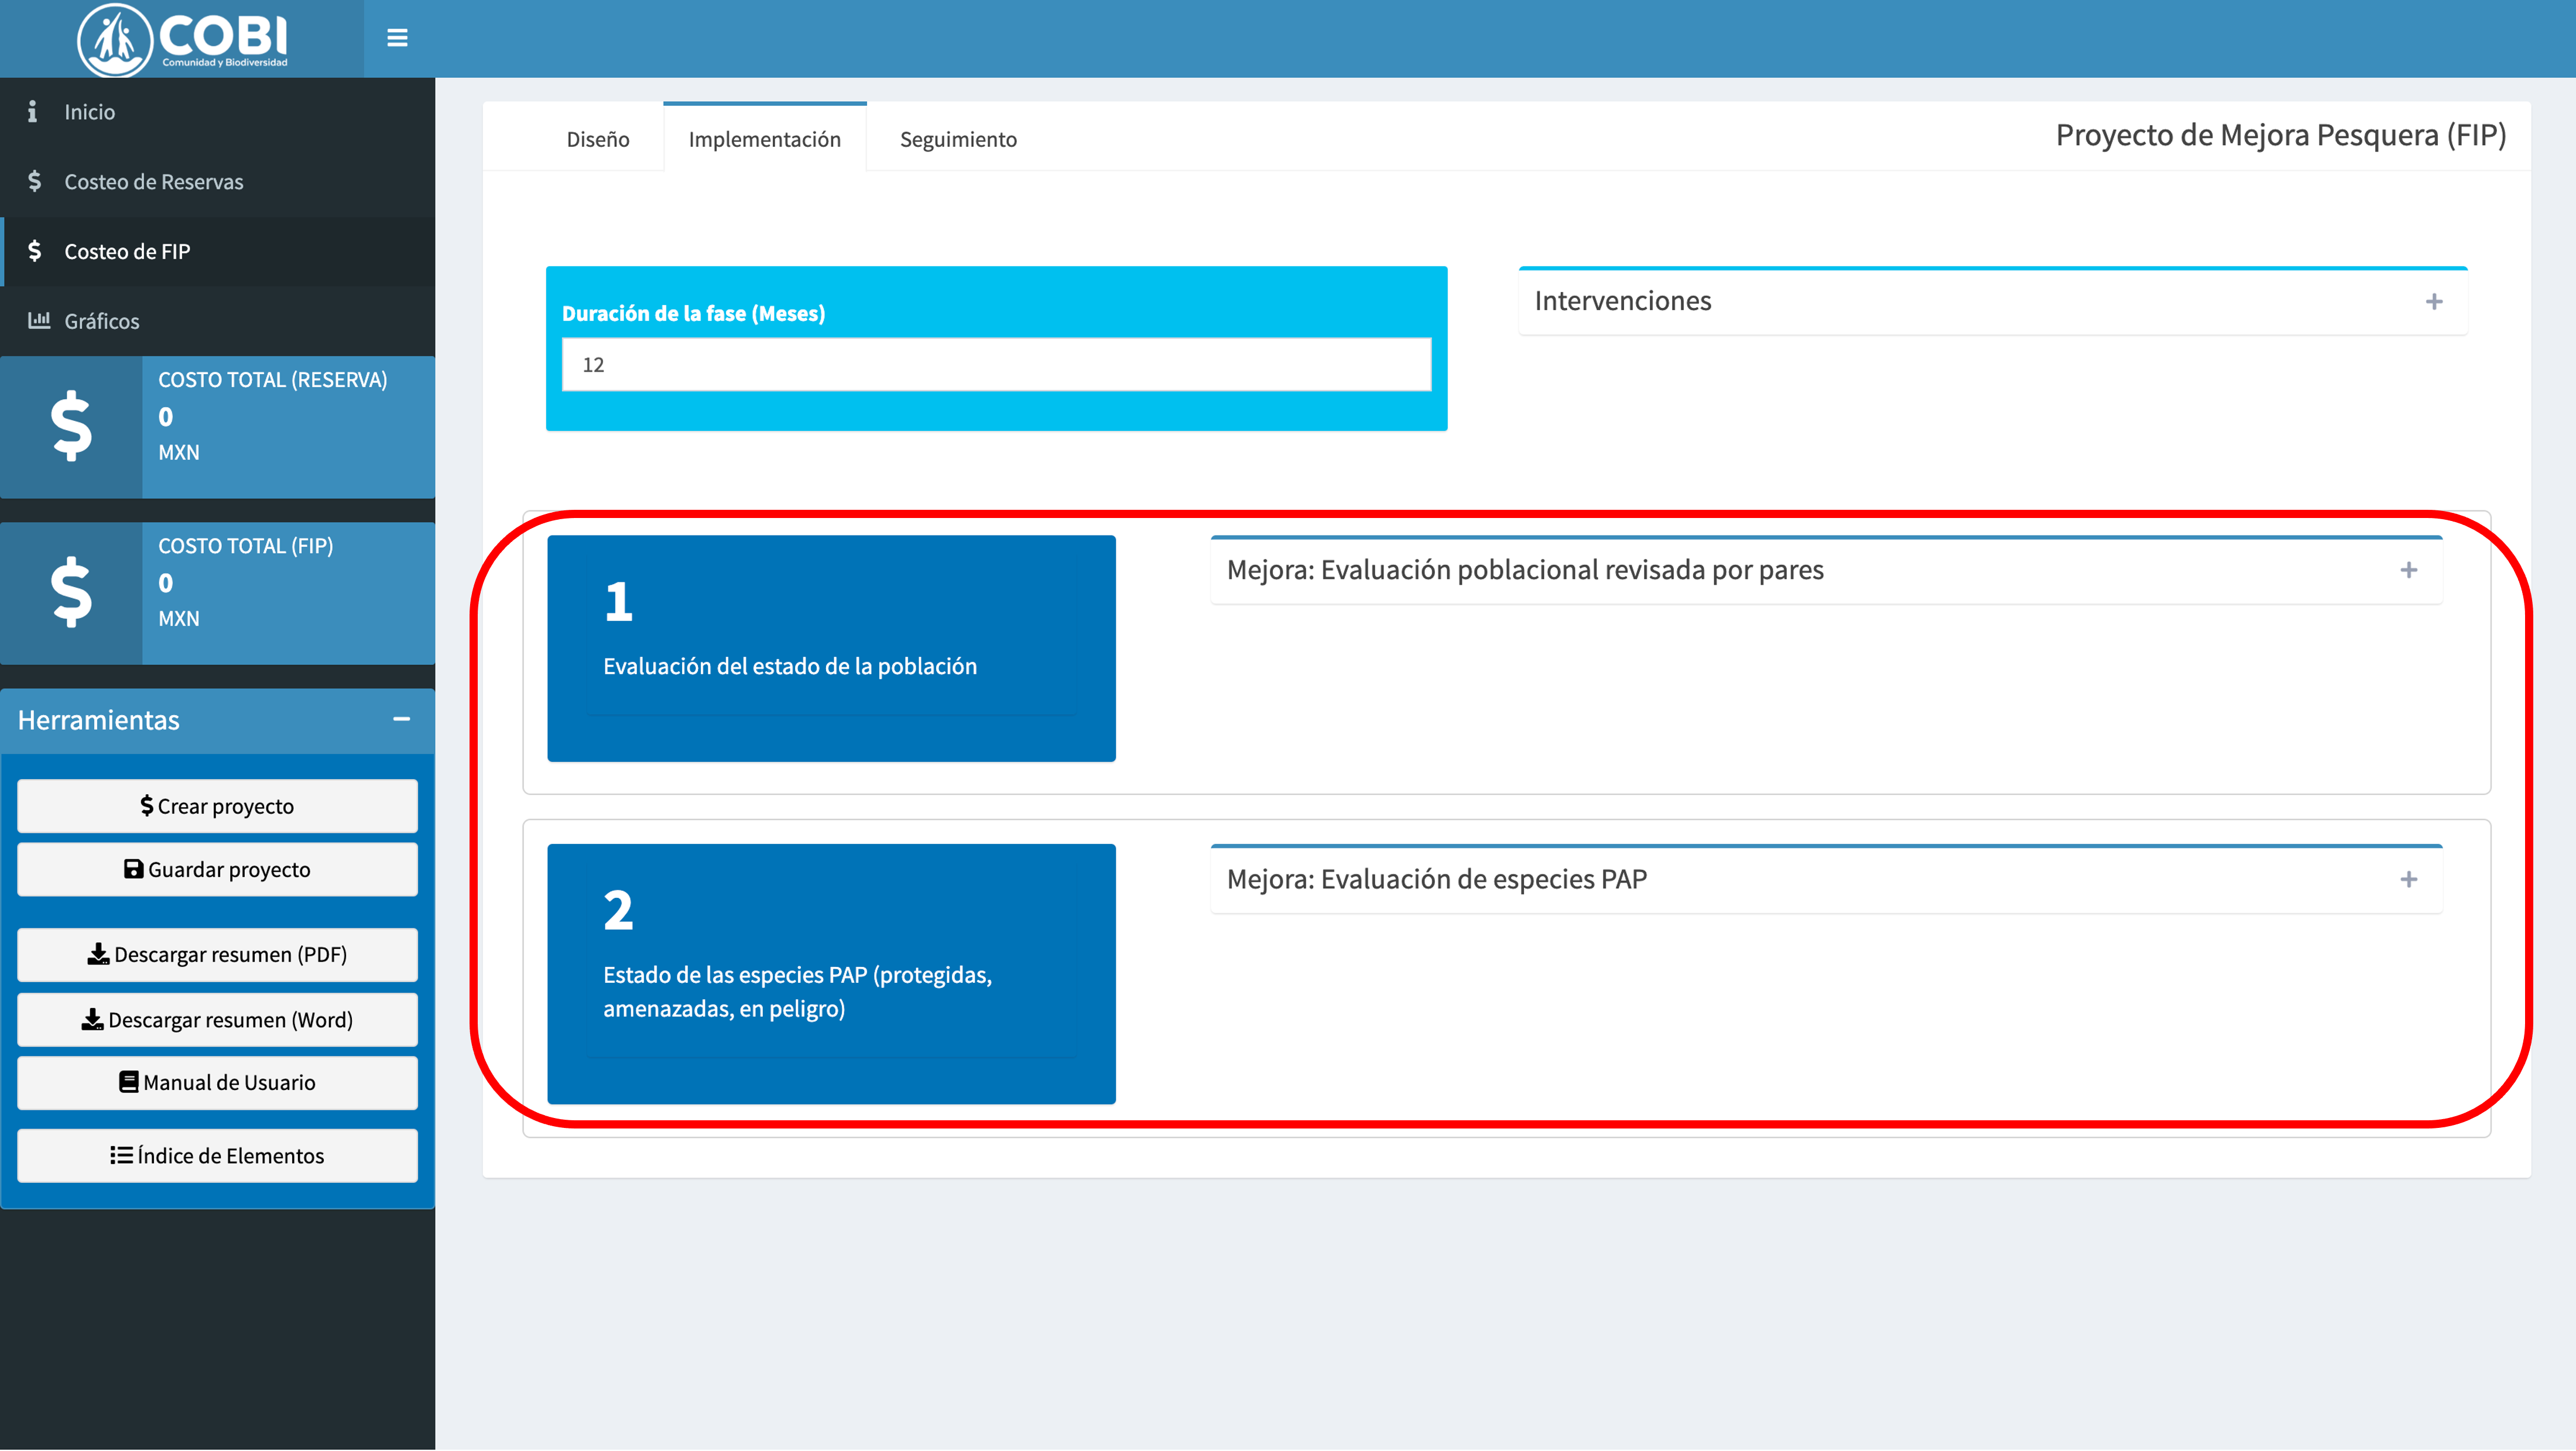
\includegraphics{images/fip-imp-5.png}
\caption{\label{fig:fip-imp-5}Generación de subfases y actividades.}
\end{figure}

\textbf{Paso 6 - } Al igual que en el caso de REMA, utiliza el botón de \textbf{+} para desplegar los elementos de la actividad y actualiza la frecuencia de la actividad (Fig \ref{fig:fip-imp-6}). En este caso es un evento único, por lo que no importa la duración de la fase, este evento no se repetirá en el tiempo.

\begin{figure}
\centering
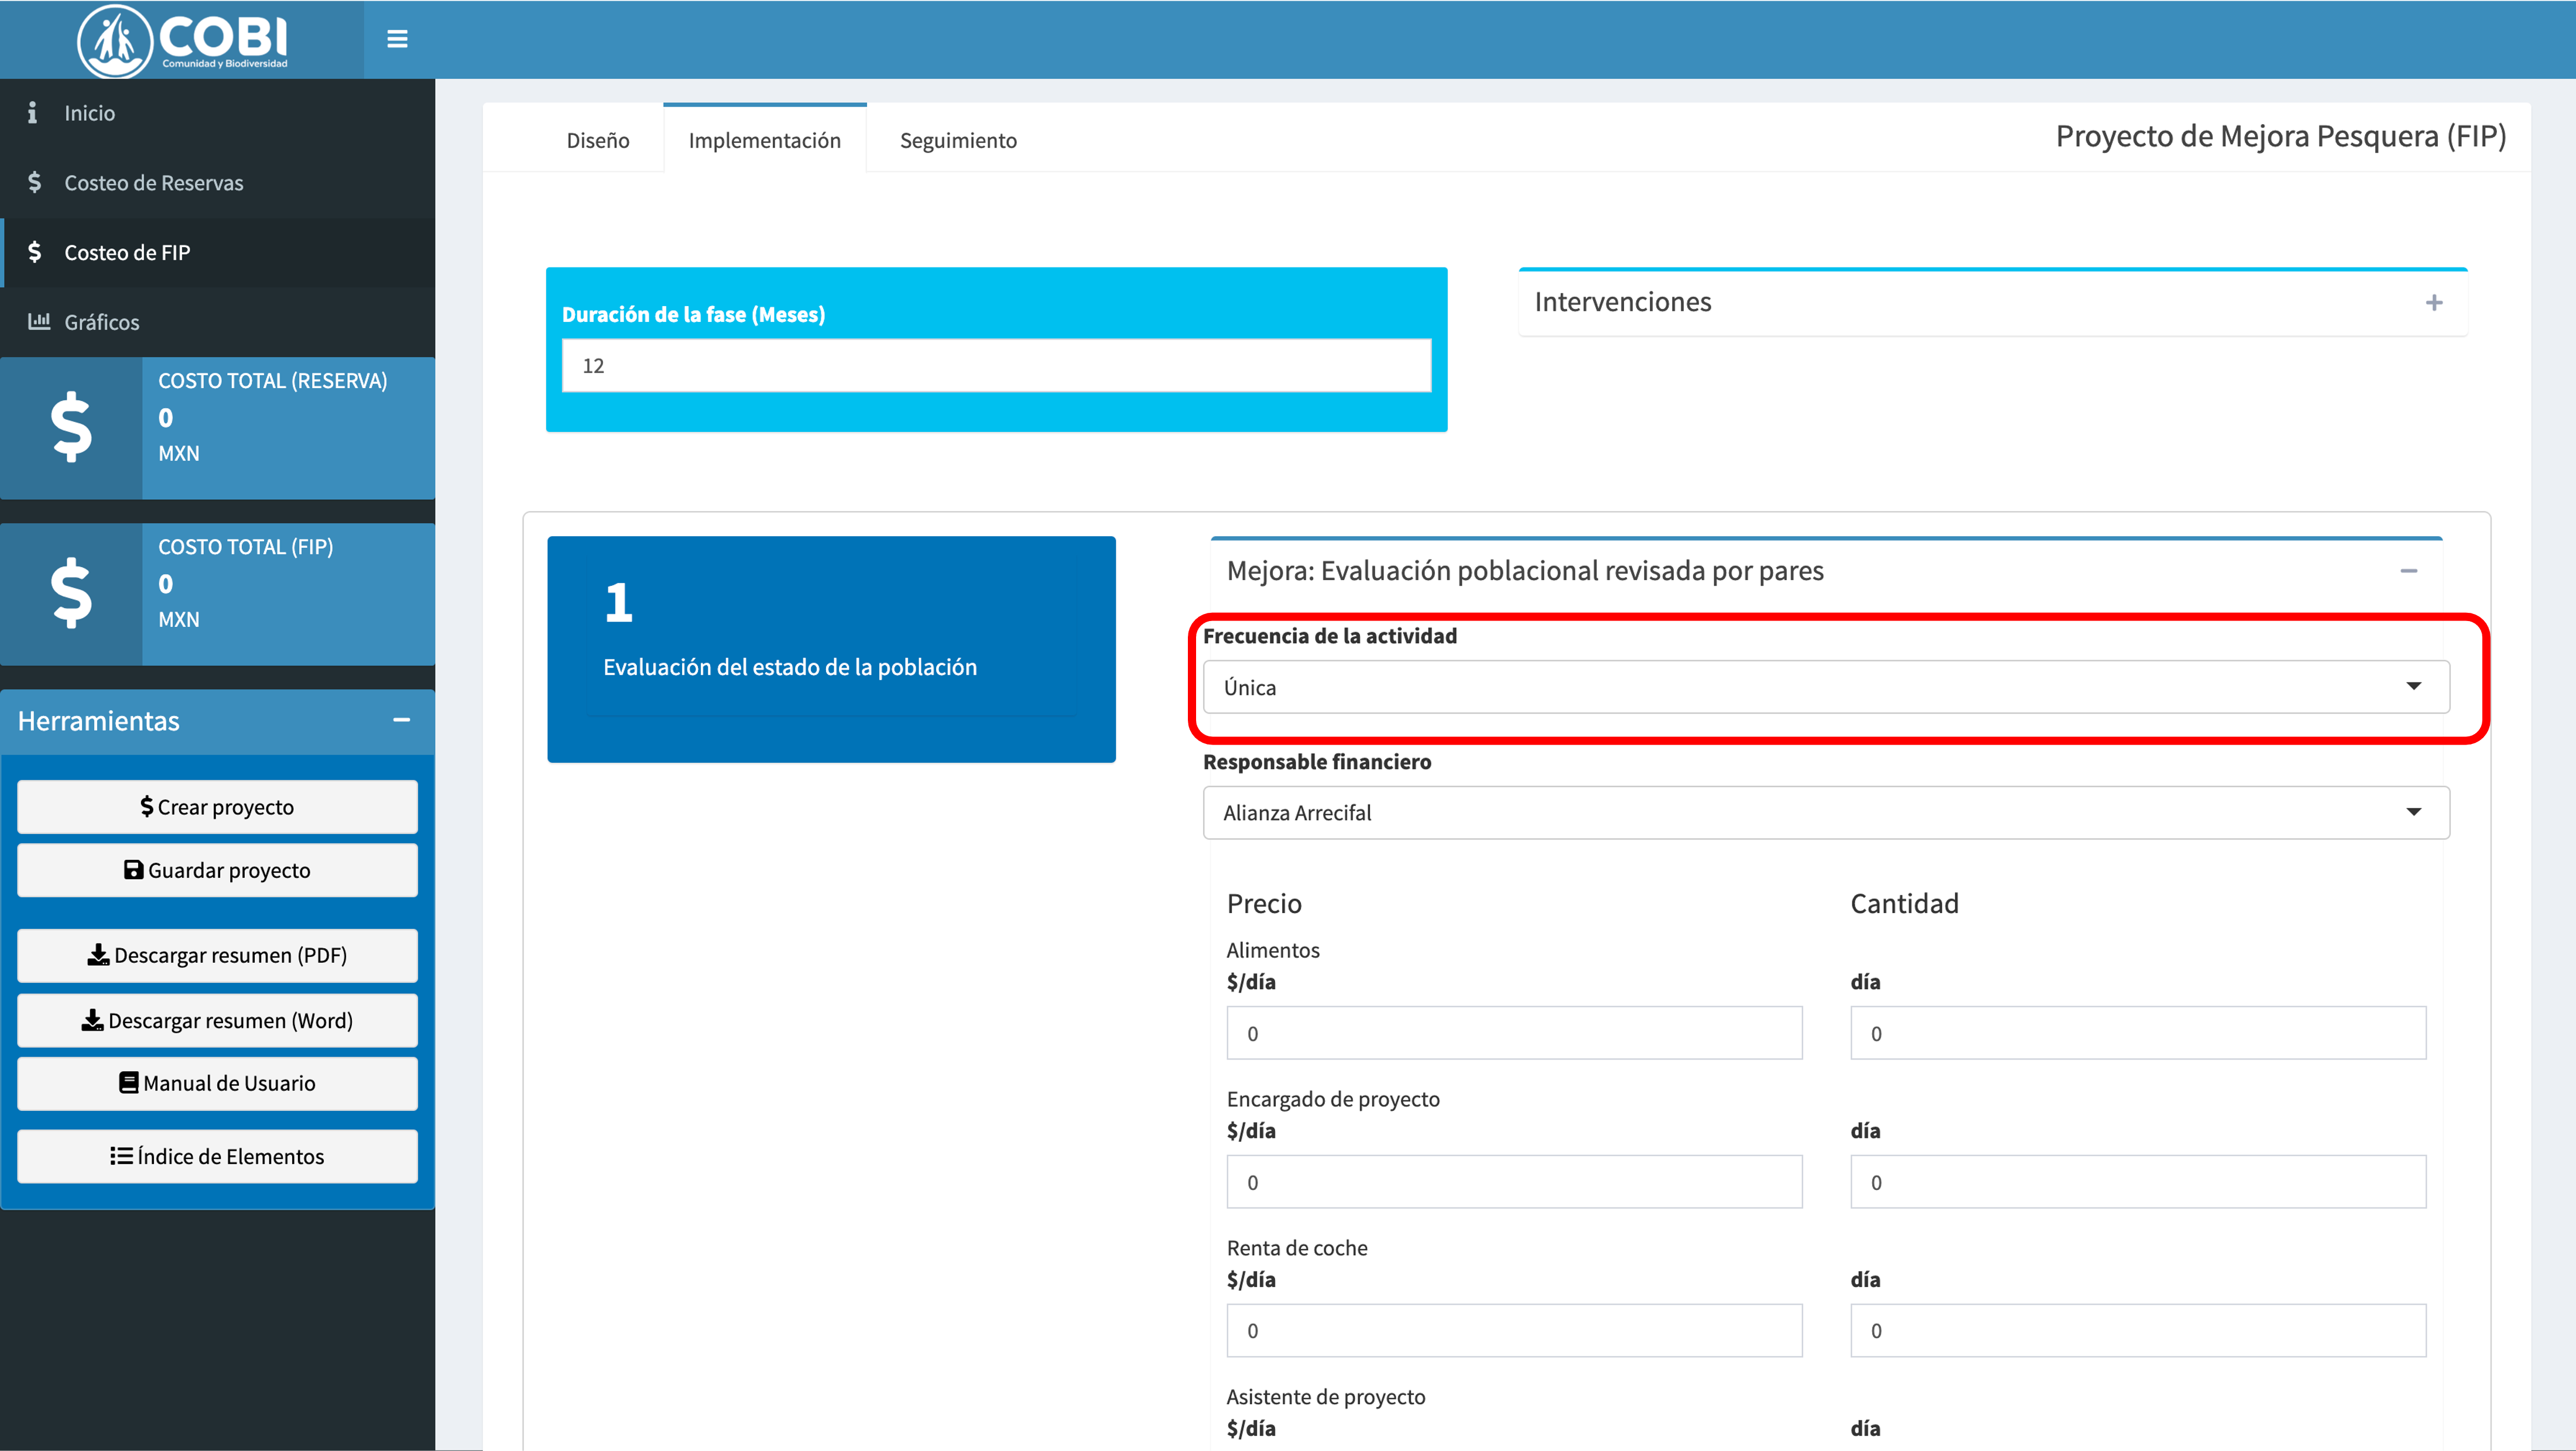
\includegraphics{images/fip-imp-6.png}
\caption{\label{fig:fip-imp-6}Selecciona la frecuencia.}
\end{figure}

\textbf{Paso 7 - } Llena los costos y cantidades de cada uno de los elementos de la actividad y observa cómo el panel izquierdo se actualiza para reflejar el costo total (Fig \ref{fig:fip-imp-7}).

\begin{figure}
\centering
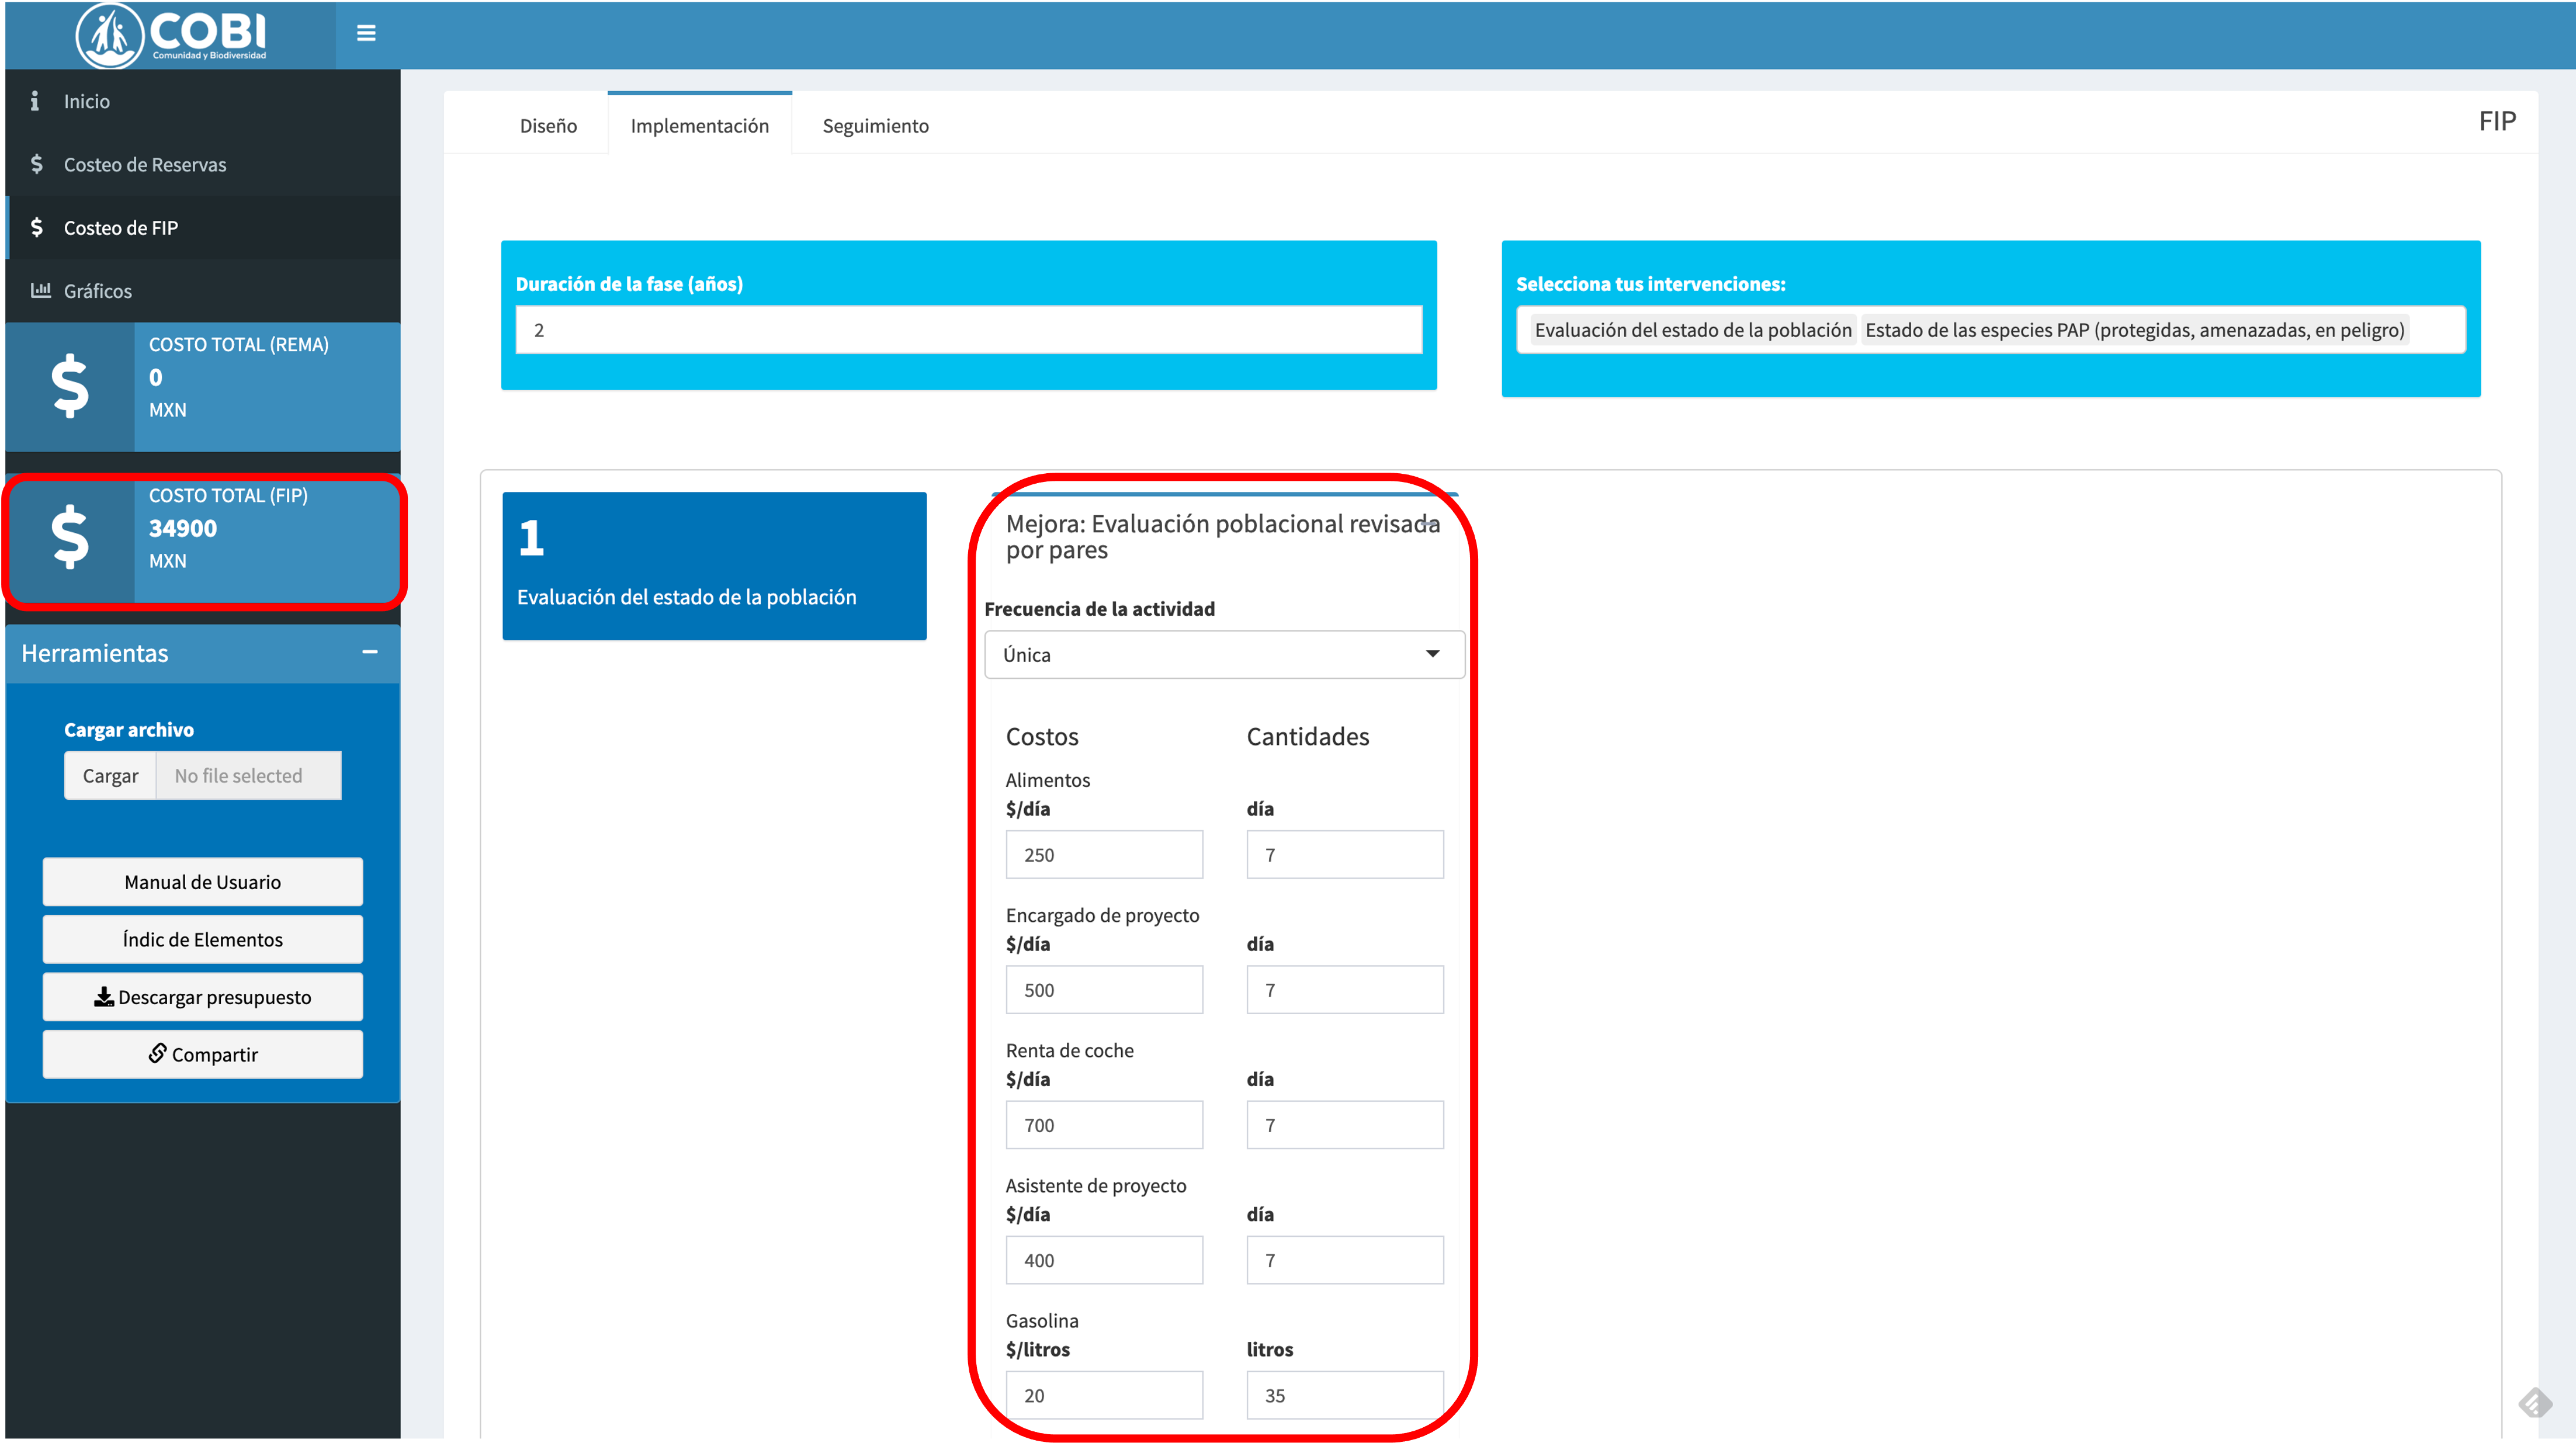
\includegraphics{images/fip-imp-7.png}
\caption{\label{fig:fip-imp-7}Llenado de datos.}
\end{figure}

\hypertarget{explorar}{%
\chapter{Explorar el presupuesto}\label{explorar}}

En el capítulo anterior vimos cómo llenar los datos. Aquí cubriremos cómo explorar las visualizaciones dentro de la app. Supongamos que ya llenamos toda la información necesaria , como lo hicimos en los ejemplos de REMA y FUP (Secciones \ref{rema} y \ref{fip}). Por lo tanto, la palicación se ve como la Figura \ref{fig:exp-1}.

\textbf{Paso 1 - } Llena los datos como lo hicimos en el capítulo anterior (Fig \ref{fig:exp-1}).

\begin{figure}
\centering
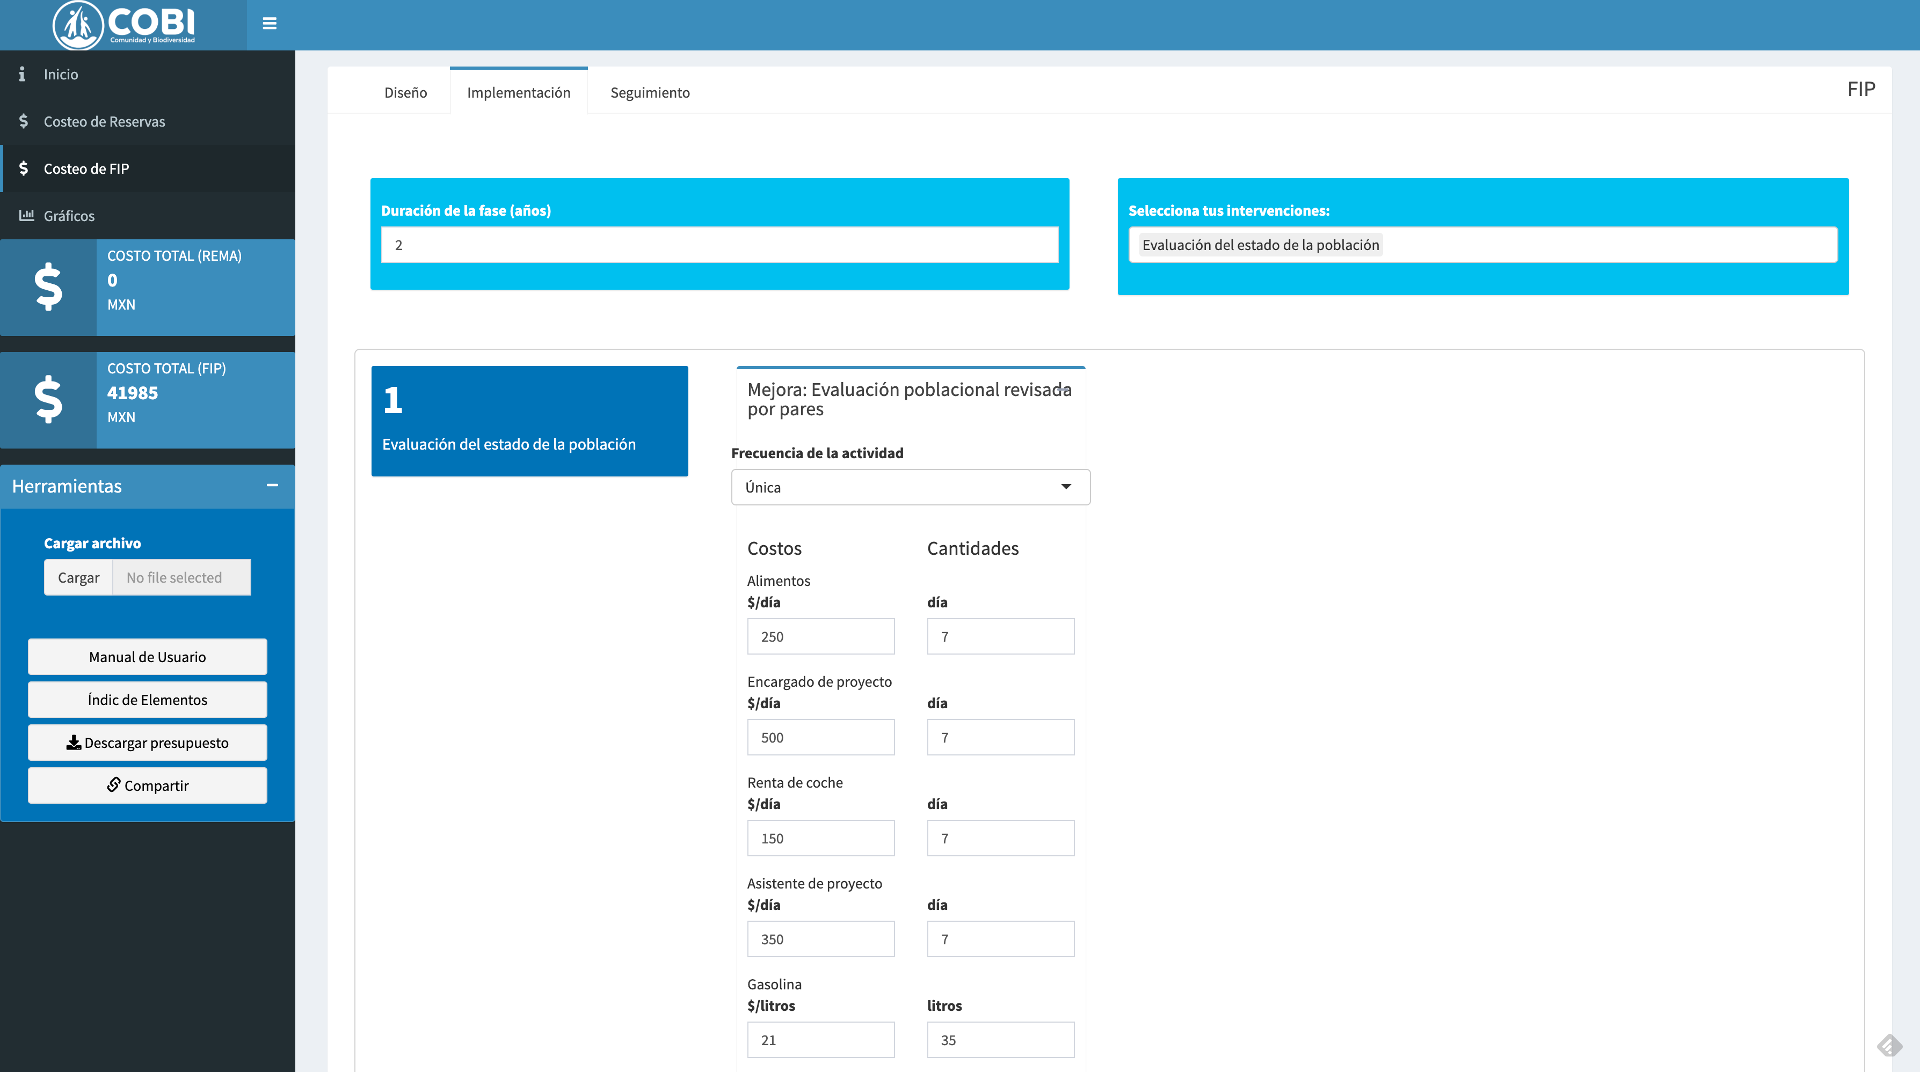
\includegraphics{images/exp-1.png}
\caption{\label{fig:exp-1}Llena el formato.}
\end{figure}

\textbf{Paso 2 - } Para explorar el presupuesto, haz click en la sección ``Gráficos'' en el panel lateral (Fig \ref{fig:exp-2}). Esto te llevará al área de trabajo de exploración. El primer panel te permite conrolar el tamaño del texto en las gráficas y cambiar el esquema de colores. El segundo te permite ver el presupuesto por fases. En este caso solamente tenemos datos para la fase de implementación, pero un presupuesto completo tendría 3 columnas (diseño, implementación y seguimiento). Los colores corresponden a los diferentes conceptos. Un ``concepto'' responde a la pregunta: ¿En qué estamos gatando el dinero?

\begin{figure}
\centering
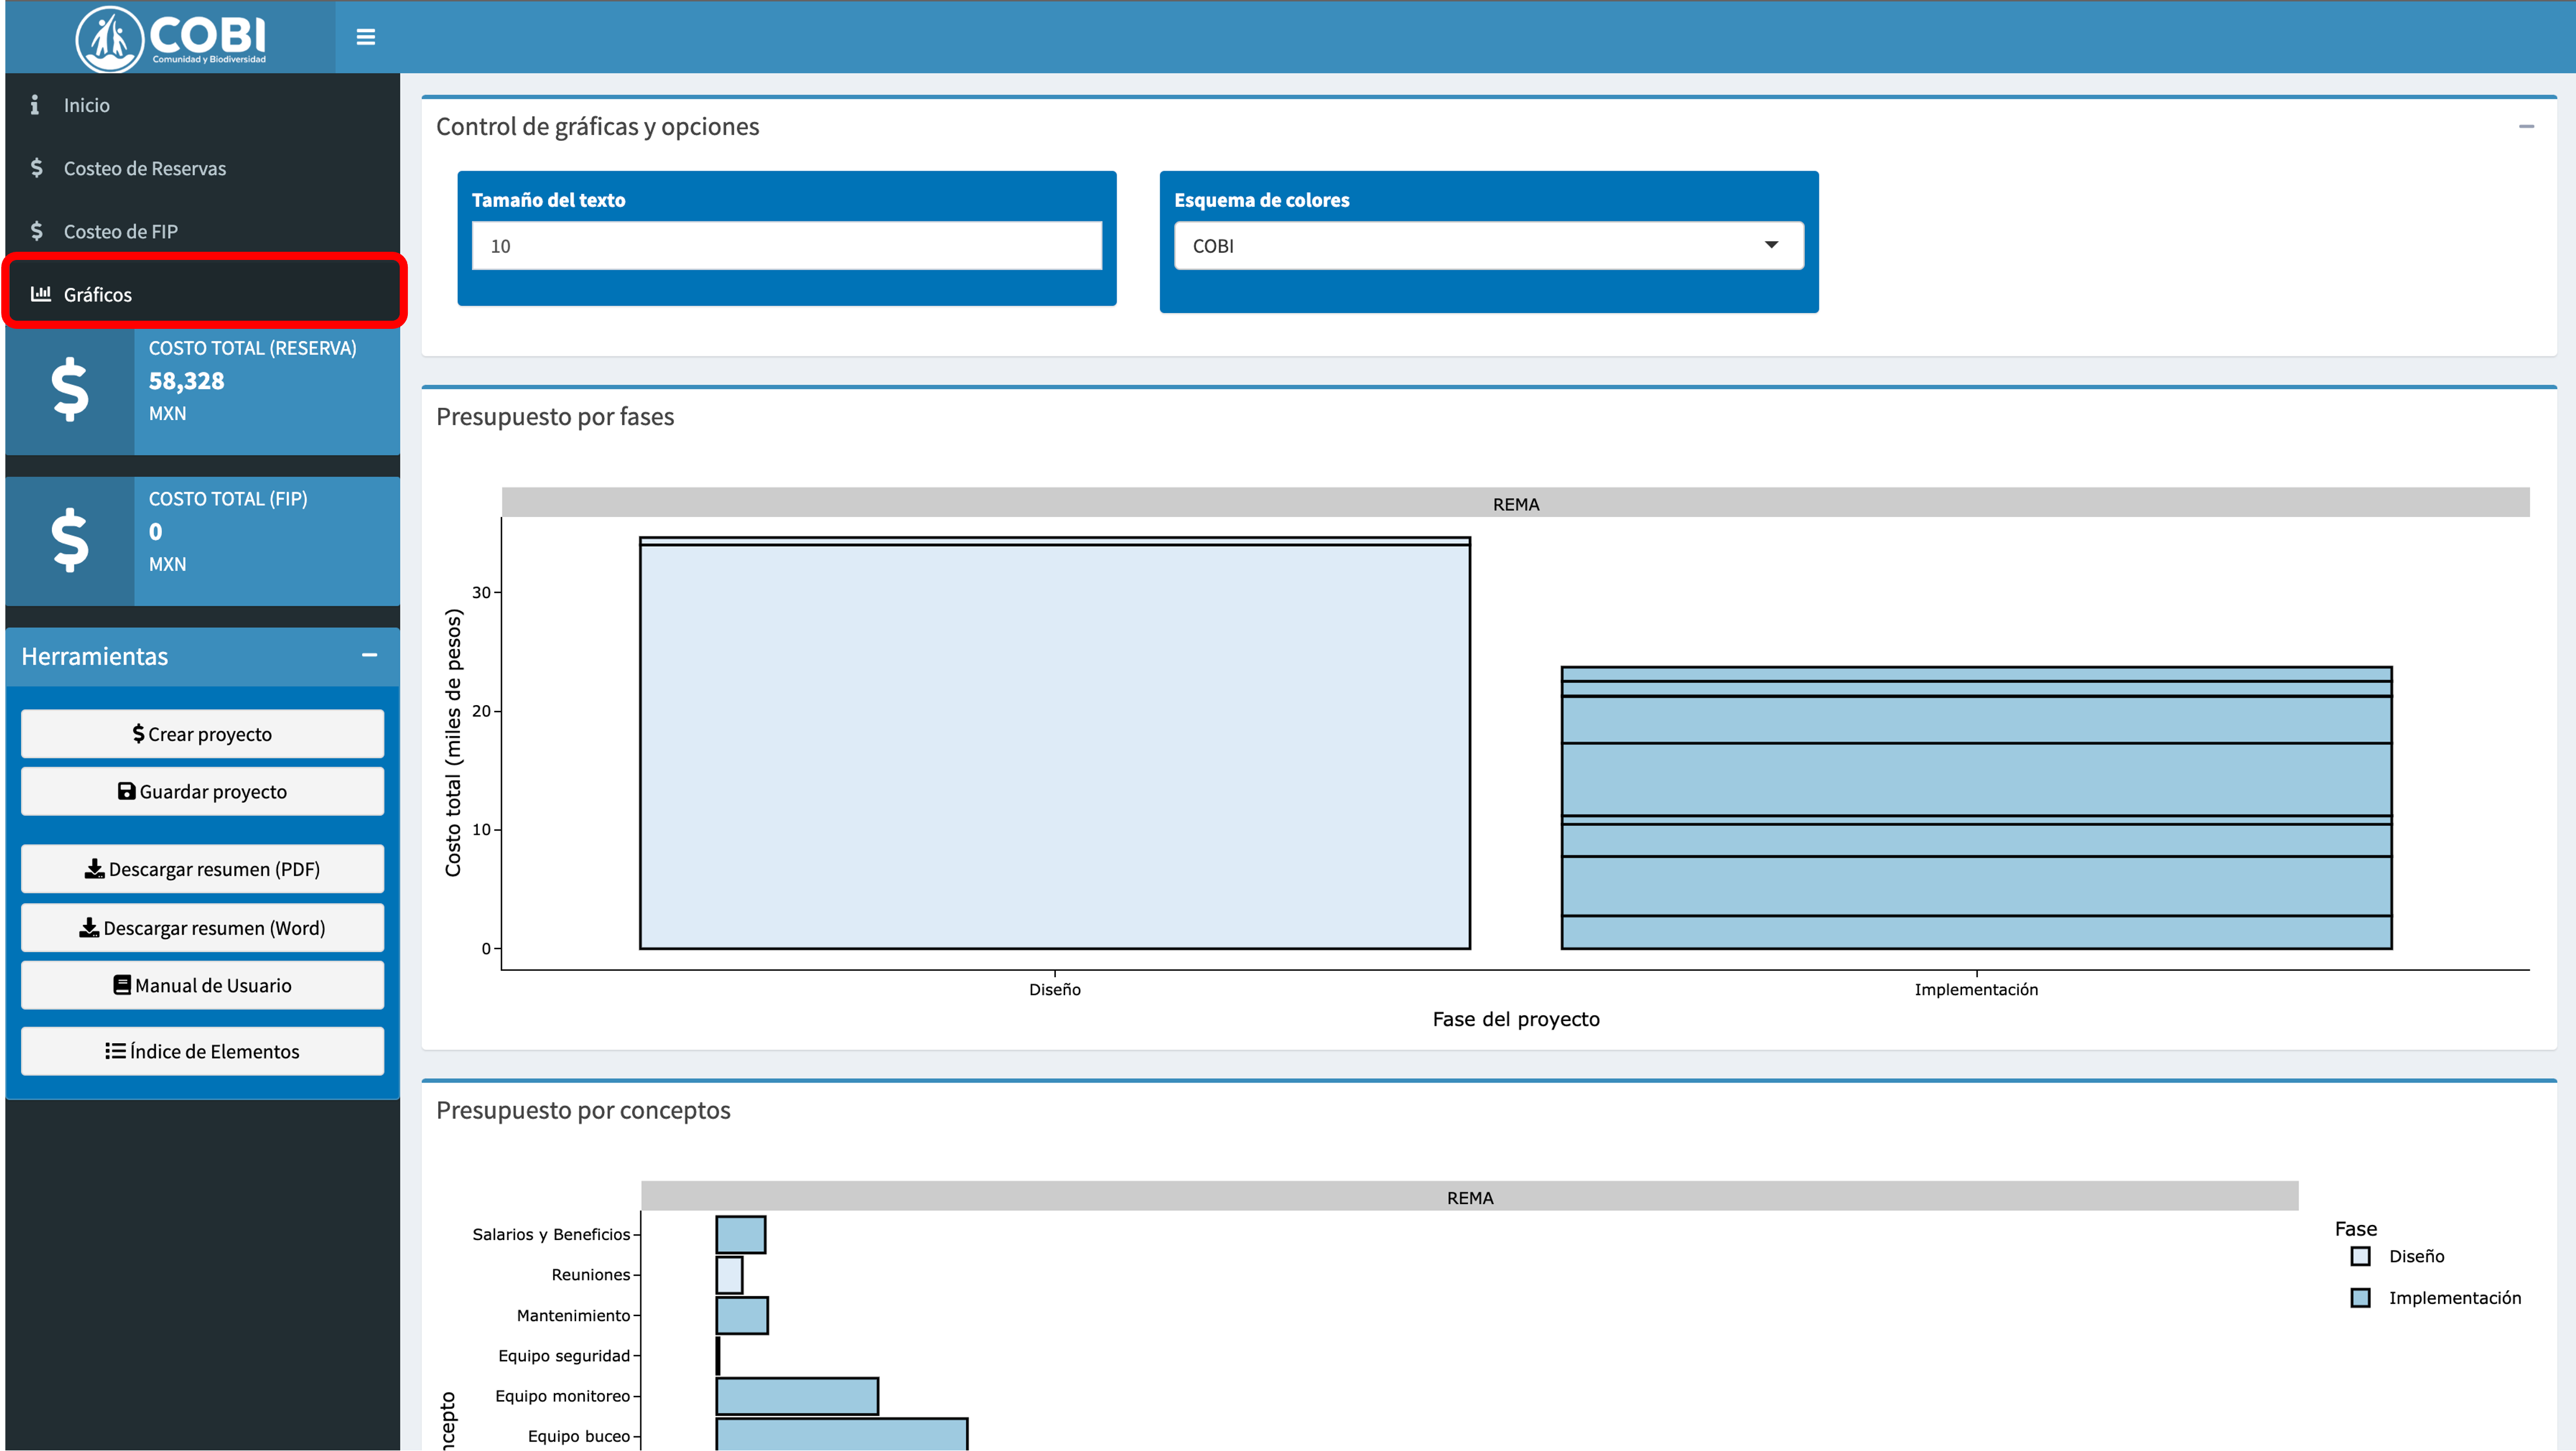
\includegraphics{images/exp-2.png}
\caption{\label{fig:exp-2}Navega a la sección de gráficos.}
\end{figure}

\textbf{Paso 3 - } Explora las gráficas con tu cursor. Al nevegar sobre los diferentes colores, puedes ver venanas con información (Fig \ref{fig:exp-3}). Por ejemplo, podemos ver que más de la mitad del presupuesto está destinado al concepto de ``Viajes y salidas a campo''.

\begin{figure}
\centering
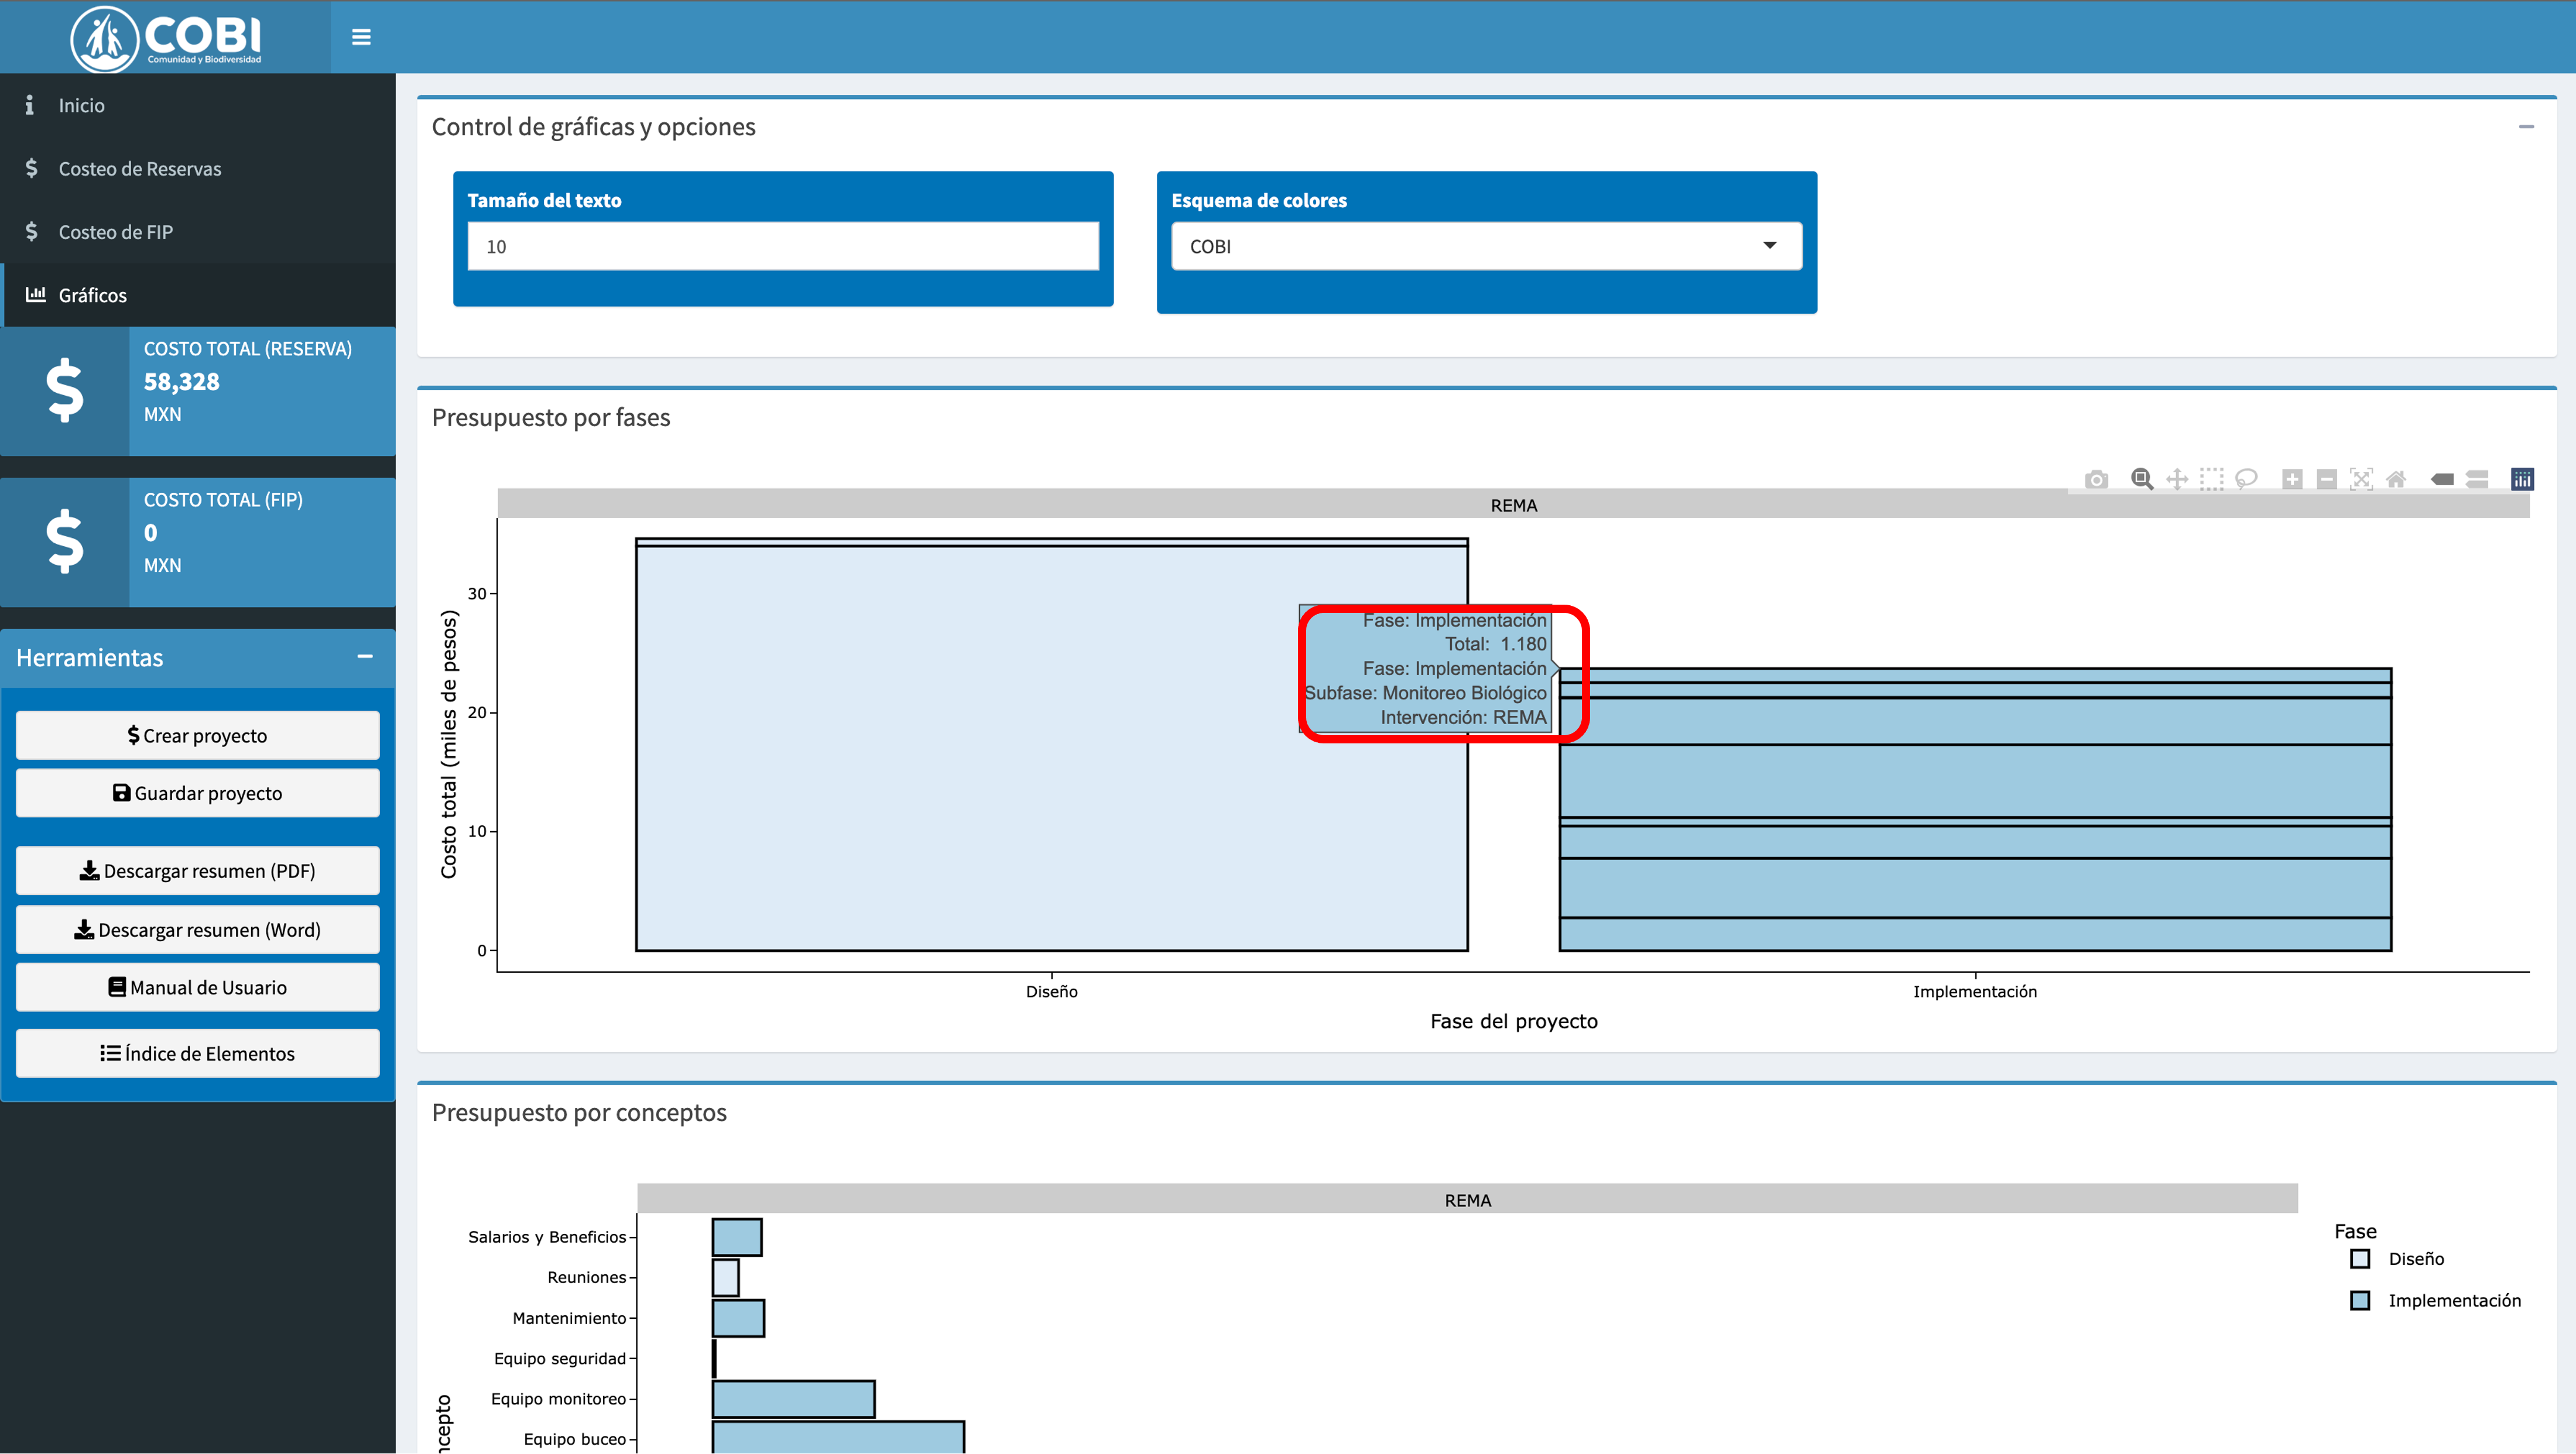
\includegraphics{images/exp-3.png}
\caption{\label{fig:exp-3}Explora los costos for fase.}
\end{figure}

\textbf{Paso 4 - } La segunda figura te muestra el resupuesto por conceptos (en el eje vertical) y el color está dado por las fases. La tercer figura te permite asignar diferentes contribuciones a los diferentes actores (Fig \ref{fig:exp-4}).

\begin{figure}
\centering
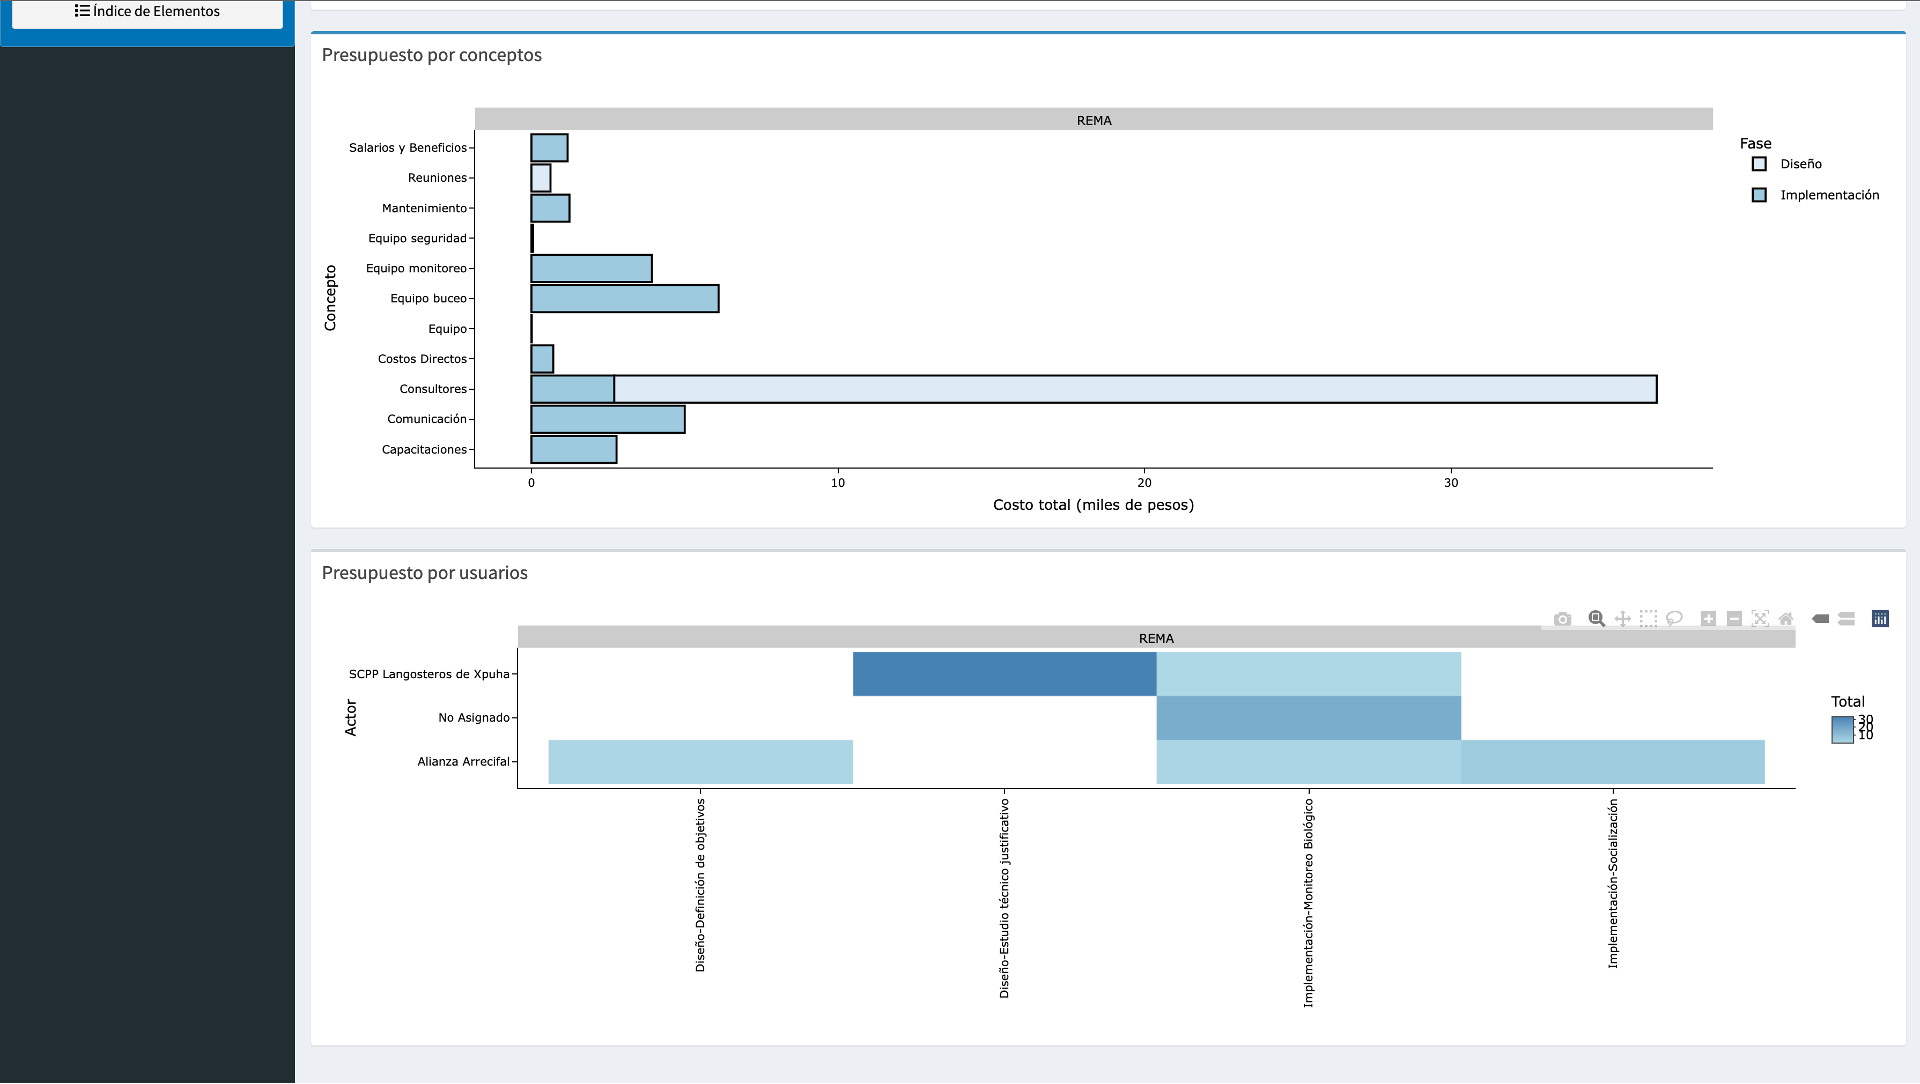
\includegraphics{images/exp-4.png}
\caption{\label{fig:exp-4}Otras gráficas.}
\end{figure}

\textbf{Paso 5 - } Modifica la división del presupuesto con 3 actores, y asigna nombres y porcentajes de conribución a cada uno (Fig \ref{fig:exp-5}).

\begin{figure}
\centering
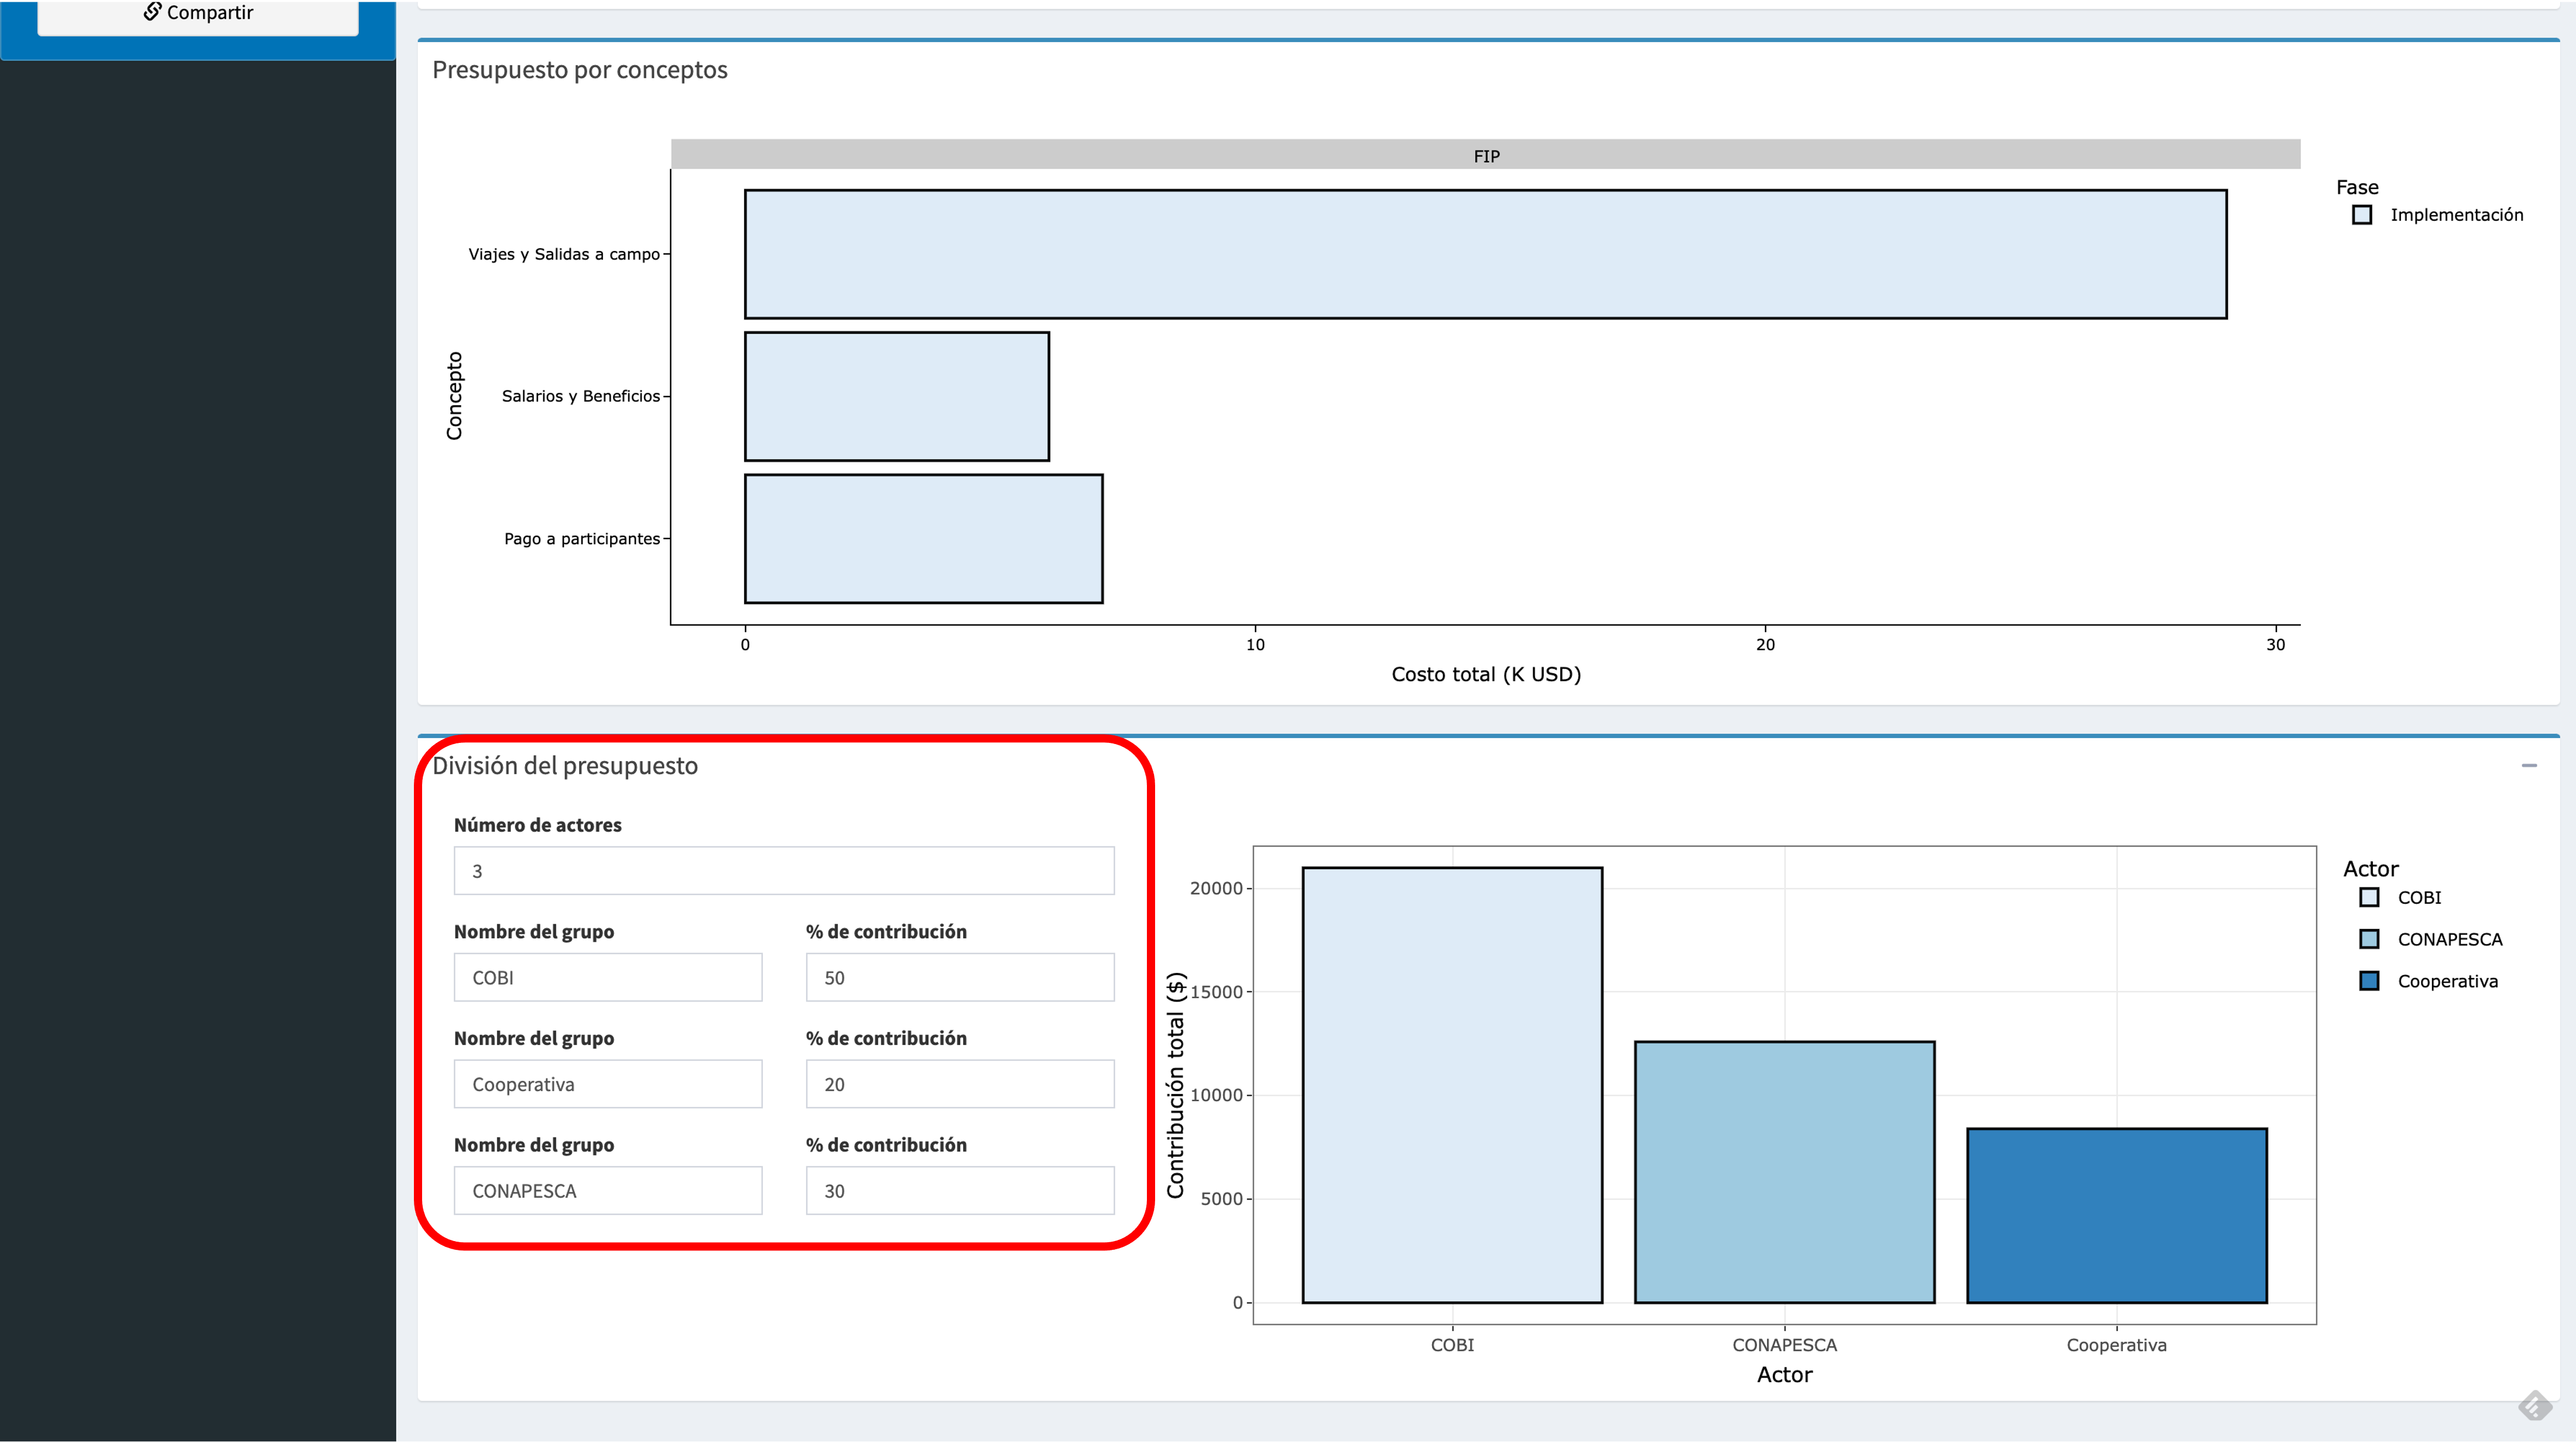
\includegraphics{images/exp-5.png}
\caption{\label{fig:exp-5}Asignar presupuesto a actores.}
\end{figure}

\hypertarget{guardar}{%
\chapter{Guardar el progreso de un presupuesto}\label{guardar}}

Una vez que llenaste y exploraste el presupuesto, puedes descargar una hoja de Excel con todos sus contenidos. Esto puede ser útil para compartir el presupuesto con alguien, o para guardar tu progreso si planeas terminar el presupuesto en otro momento.

Para descargar el presupuesto, simplemente haz click en el botón de ``Descargar presupuesto'' en el planel lateral izquierdo (Fig \ref{fig:down-1}).

\begin{figure}
\centering
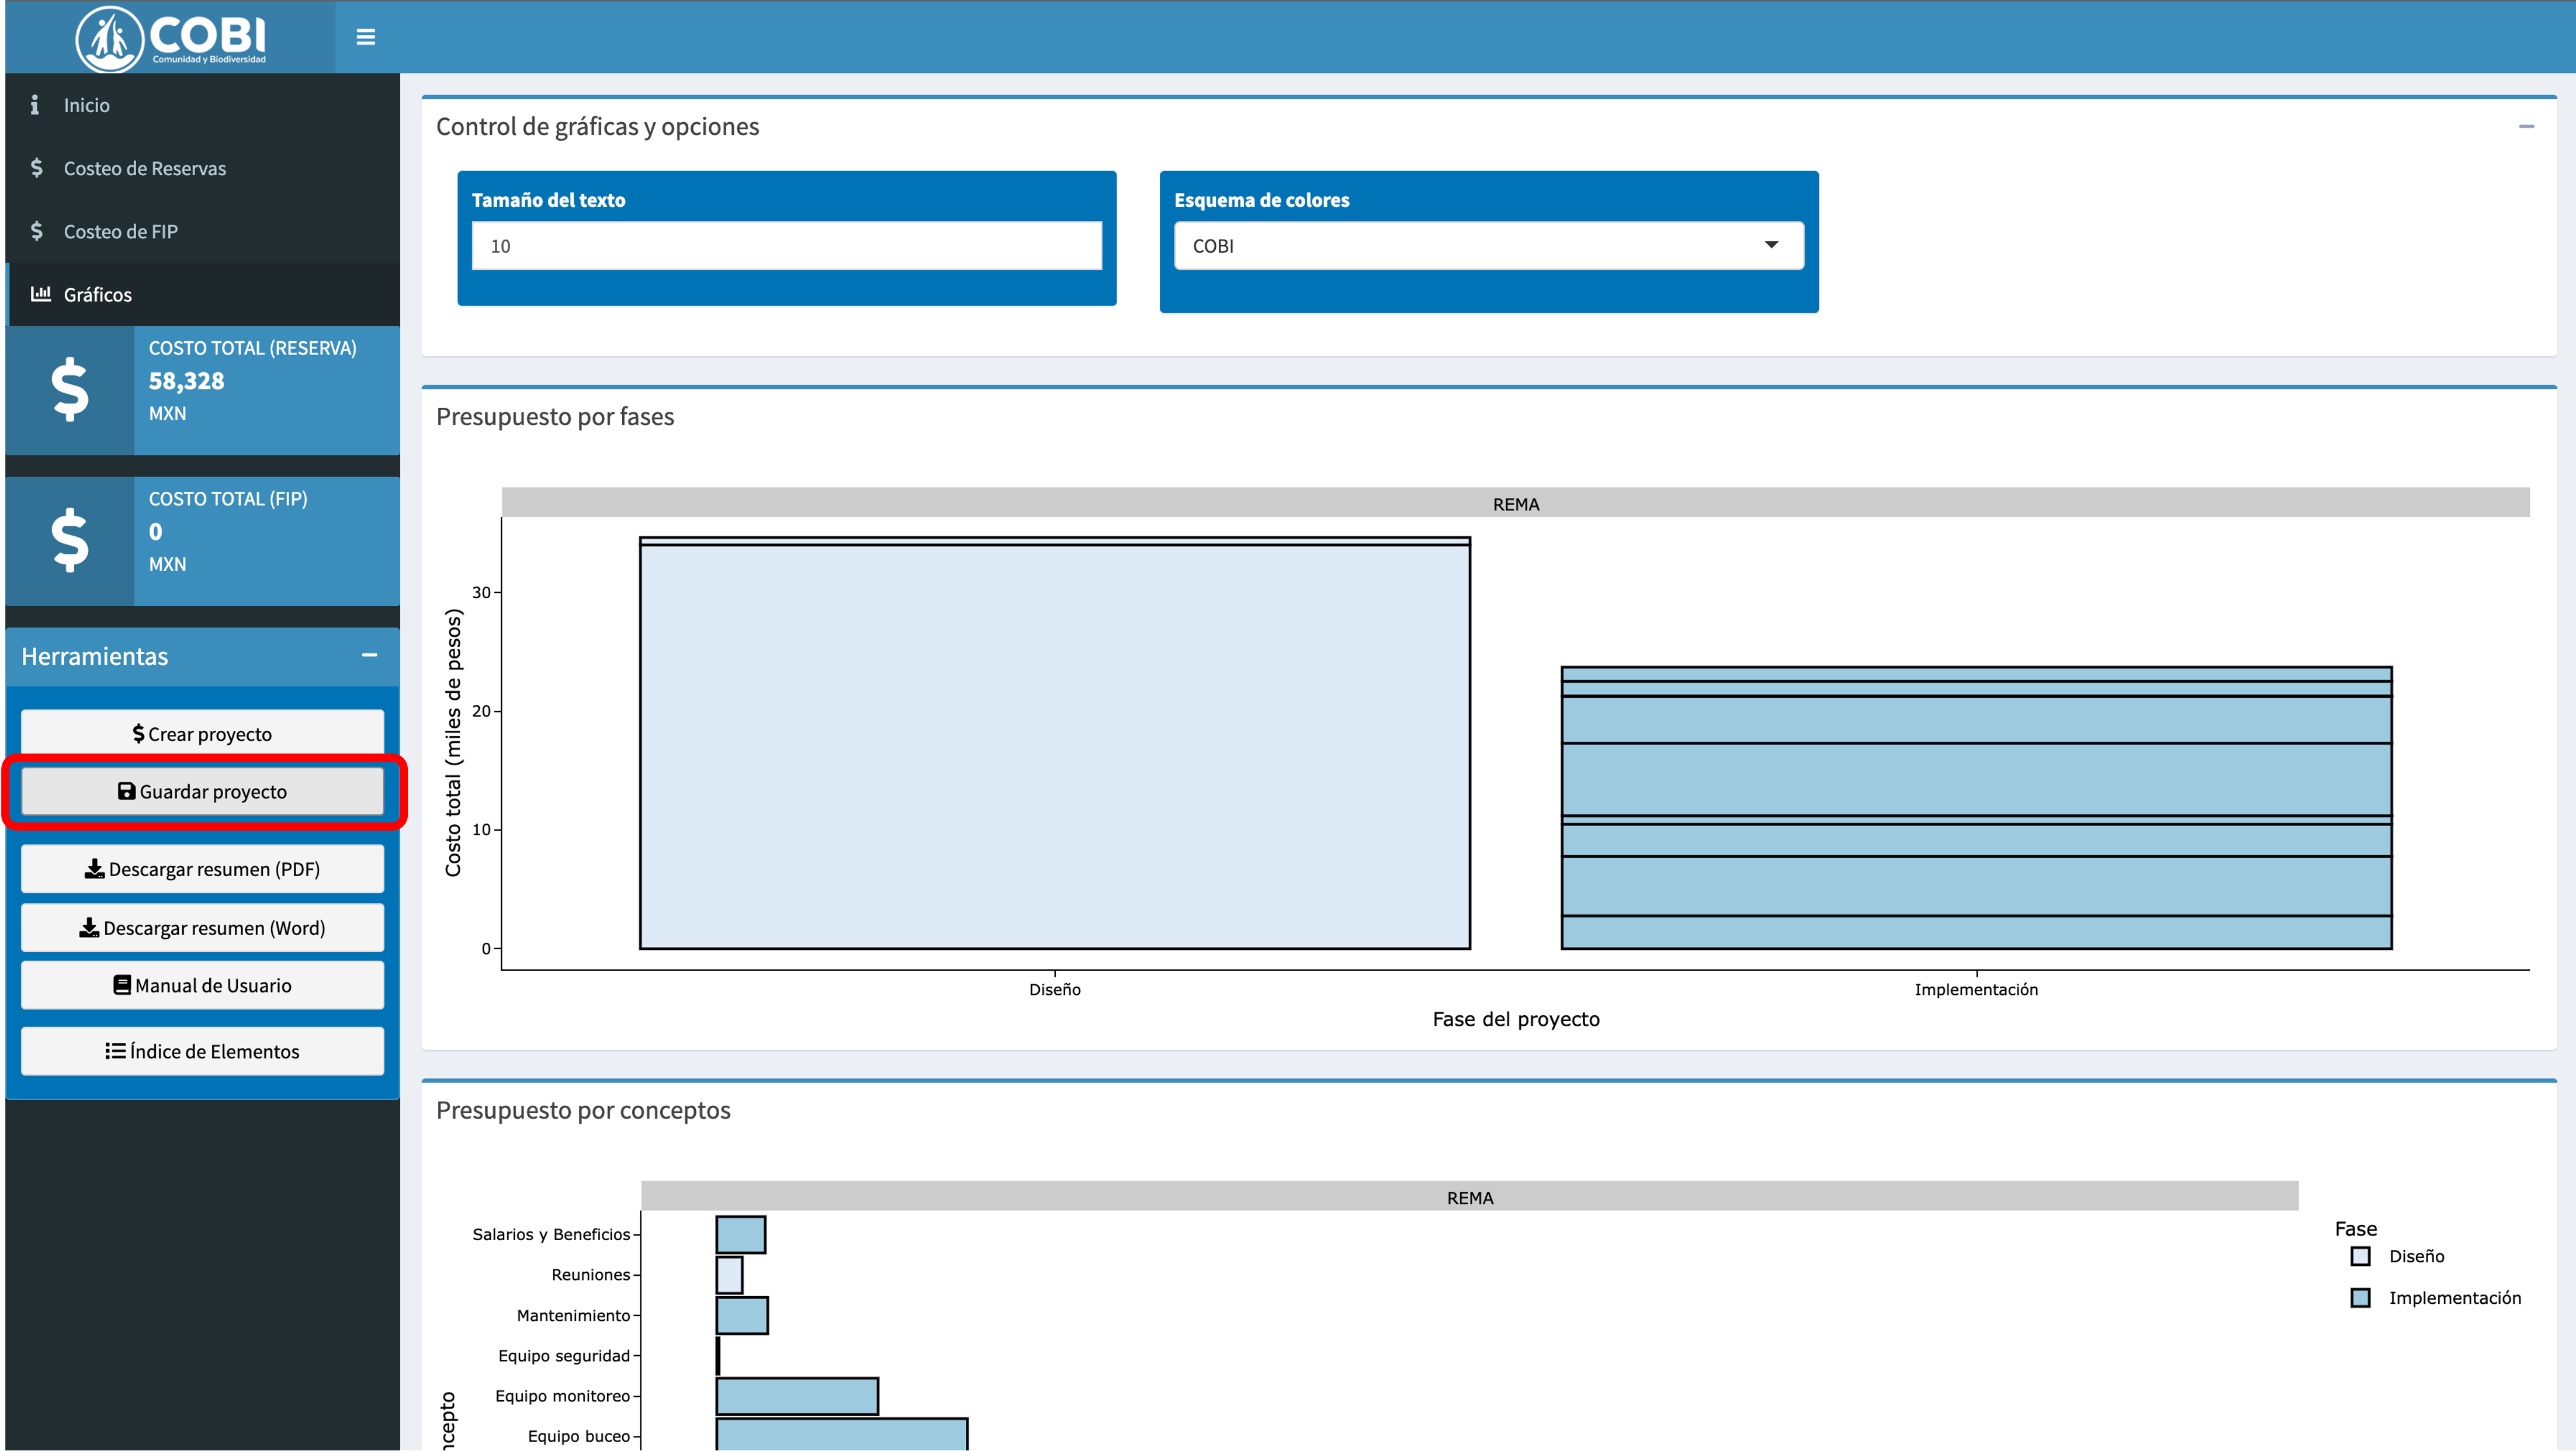
\includegraphics{images/down-1.png}
\caption{\label{fig:down-1}Botón para descargar.}
\end{figure}

Dependiendo de las opciones de tu explorador, el archivo se va a descargar a tu folder de descargas, o un explorador se abrirá para permitirte elegir un lugar para descargar los datos y asignar un nombre al archivo (Fig \ref{fig:down-2}). \textbf{NOTA IMPRTANTE: Si planeas re-utilizar este presupuesto para continuar modificaciones, es importante NO modificar manualmente los contenidos.}

\begin{figure}
\centering
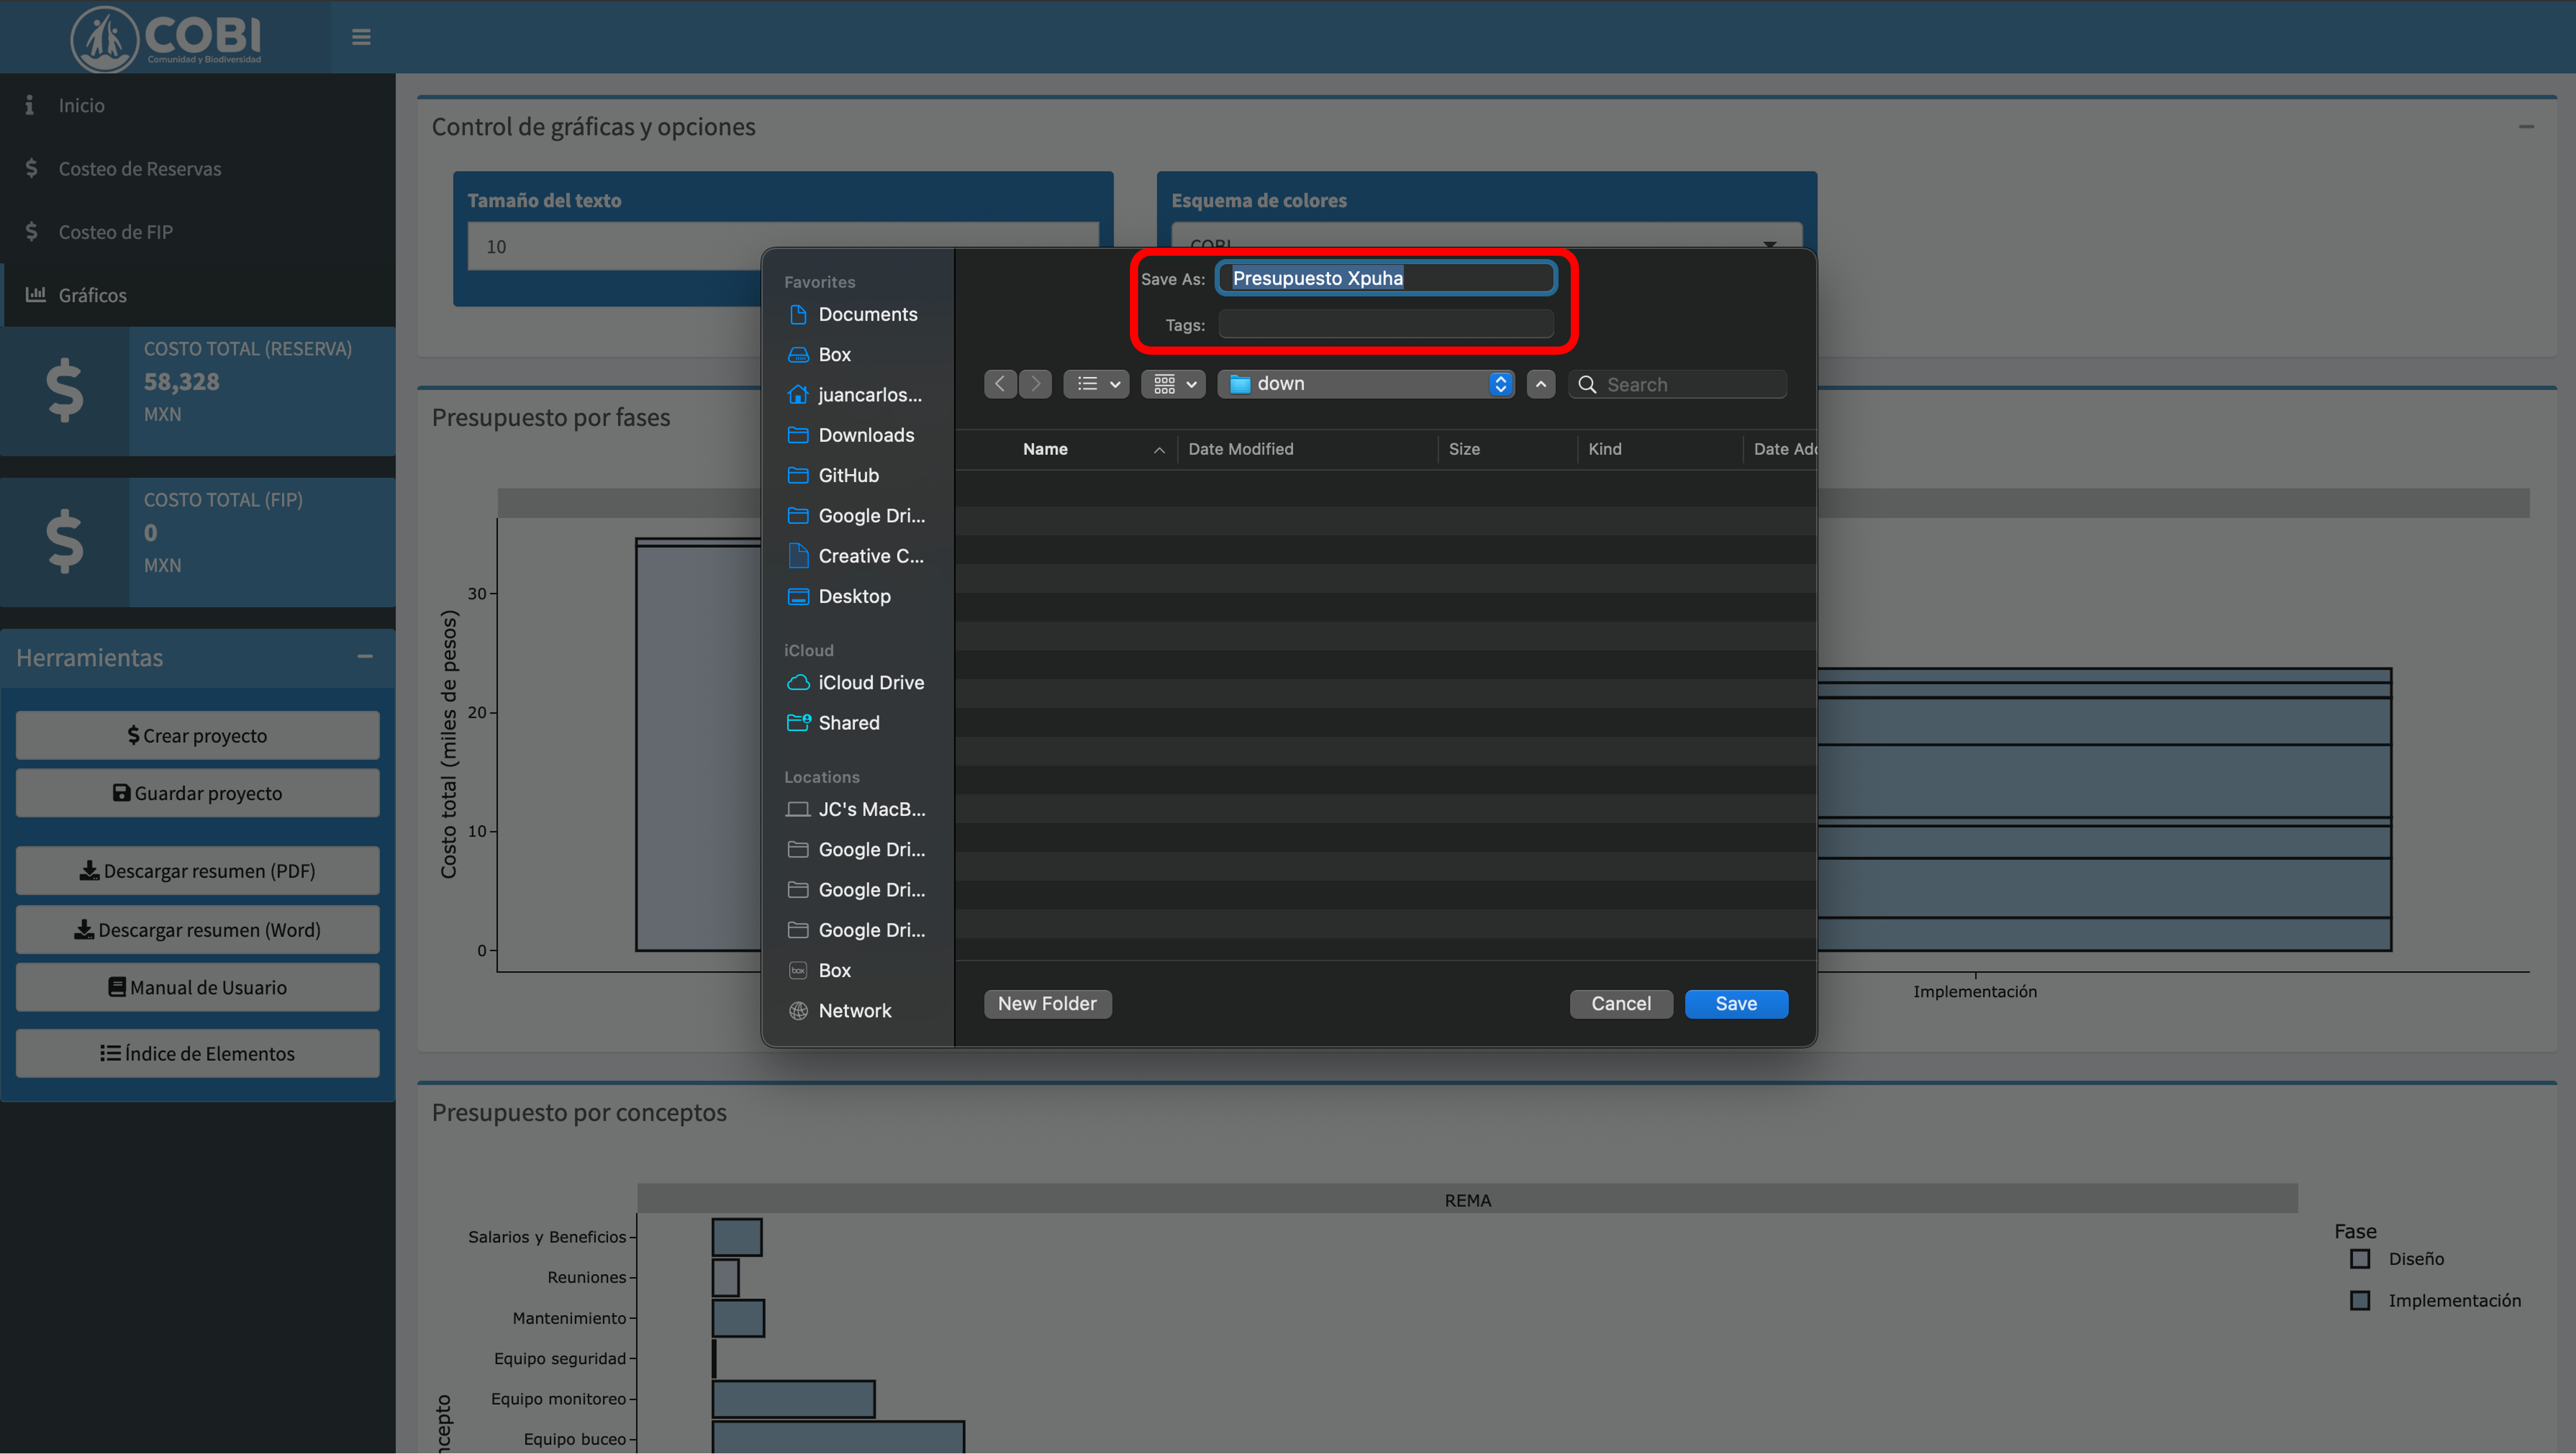
\includegraphics{images/down-2.png}
\caption{\label{fig:down-2}Ventana de descarga.}
\end{figure}

\hypertarget{cargar}{%
\chapter{Cargar el estado de un presupuesto anterior}\label{cargar}}

La nueva versión de la app te permite cargar un archivo de presupuesto para automáticamente llenar los campos de la app. Esto puede ser útil si trabajarás varios días en la elaboración de un presupuesto y necesitas hacerlo en varias sesiones. También puede ser útil si tu organización desea elaborar un formato predeterminado de costos y cantidades para ciertas actividades.

\textbf{Paso 1 - } Para cargar un presupuesto, empeiza con una sesión nueva donde todos los campos estén vacíos. En el panel lateral izquierdo, haz click n el botón de ``Cargar'' \ref{fig:up-1}).

\begin{figure}
\centering
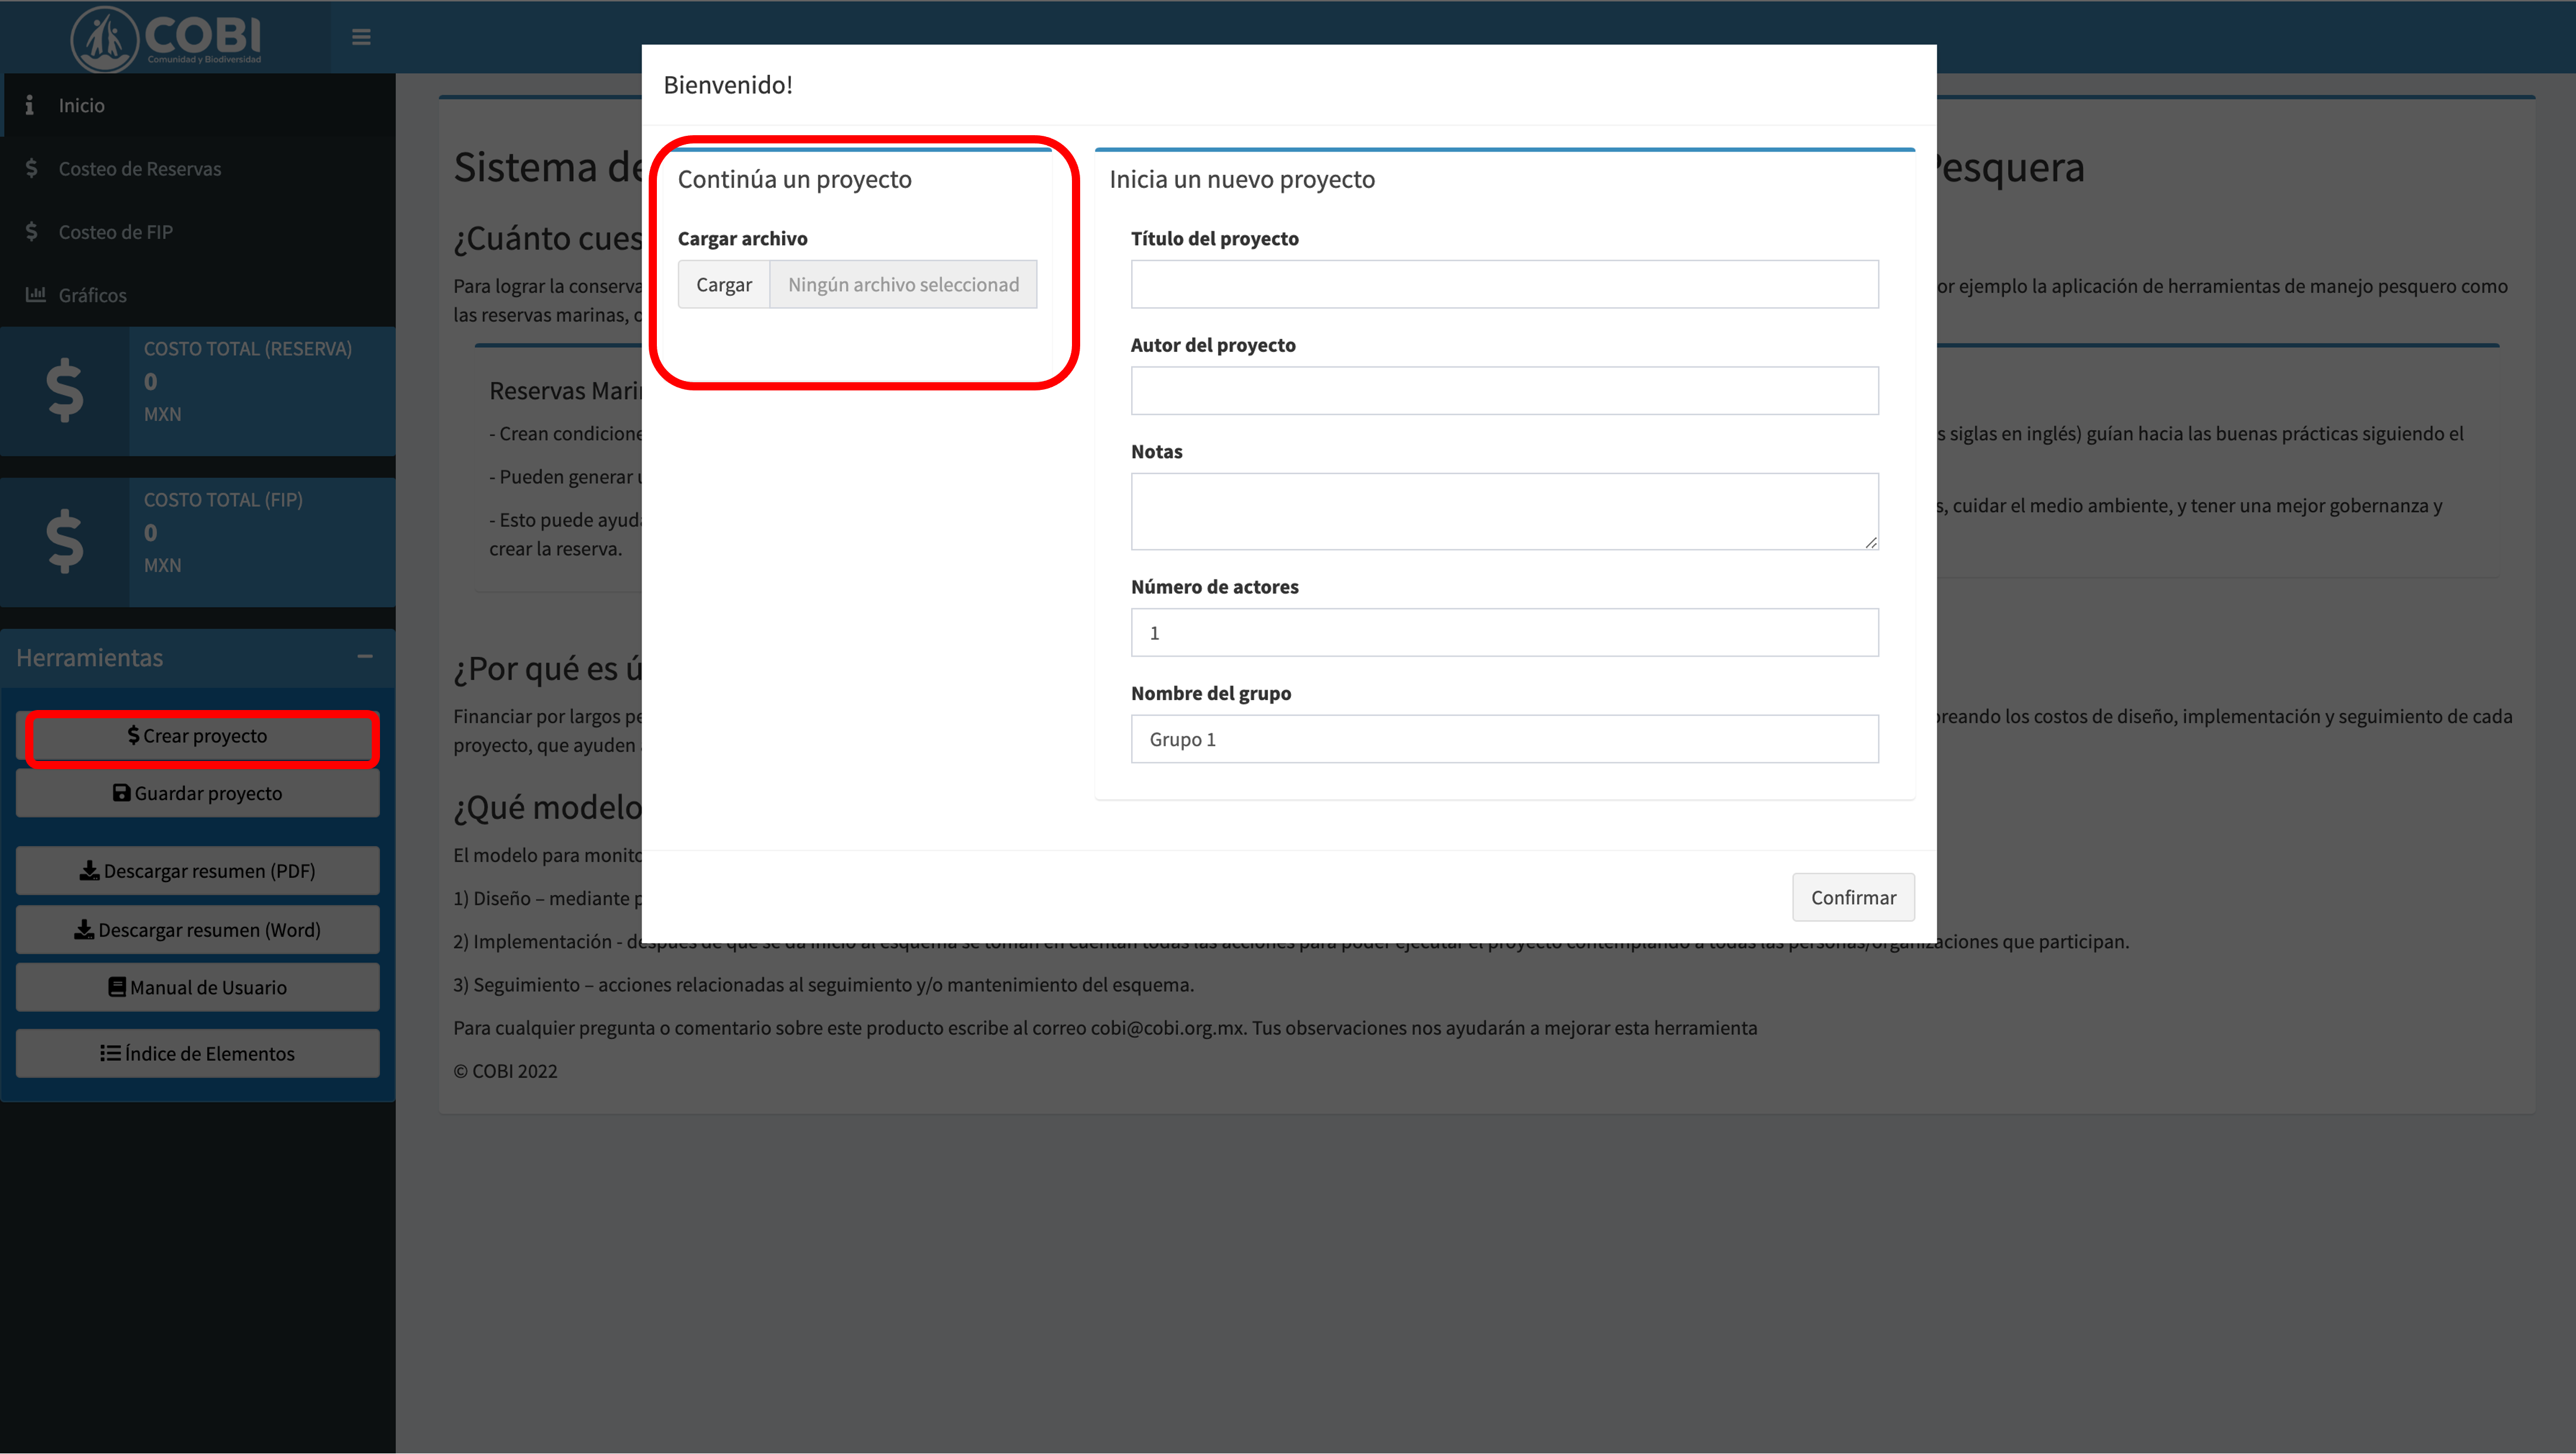
\includegraphics{images/up-1.png}
\caption{\label{fig:up-1}Empieza con una sesión nueva.}
\end{figure}

\textbf{Paso 2 - } Selecciona el archivo de presupuesto que deseas cargar \ref{fig:up-2}). En este ejemplo, estoy seleccionando un presupuesto de FIP, que se enfoca en la fase de implementación de una evaluación del estado del recurso.

\begin{figure}
\centering
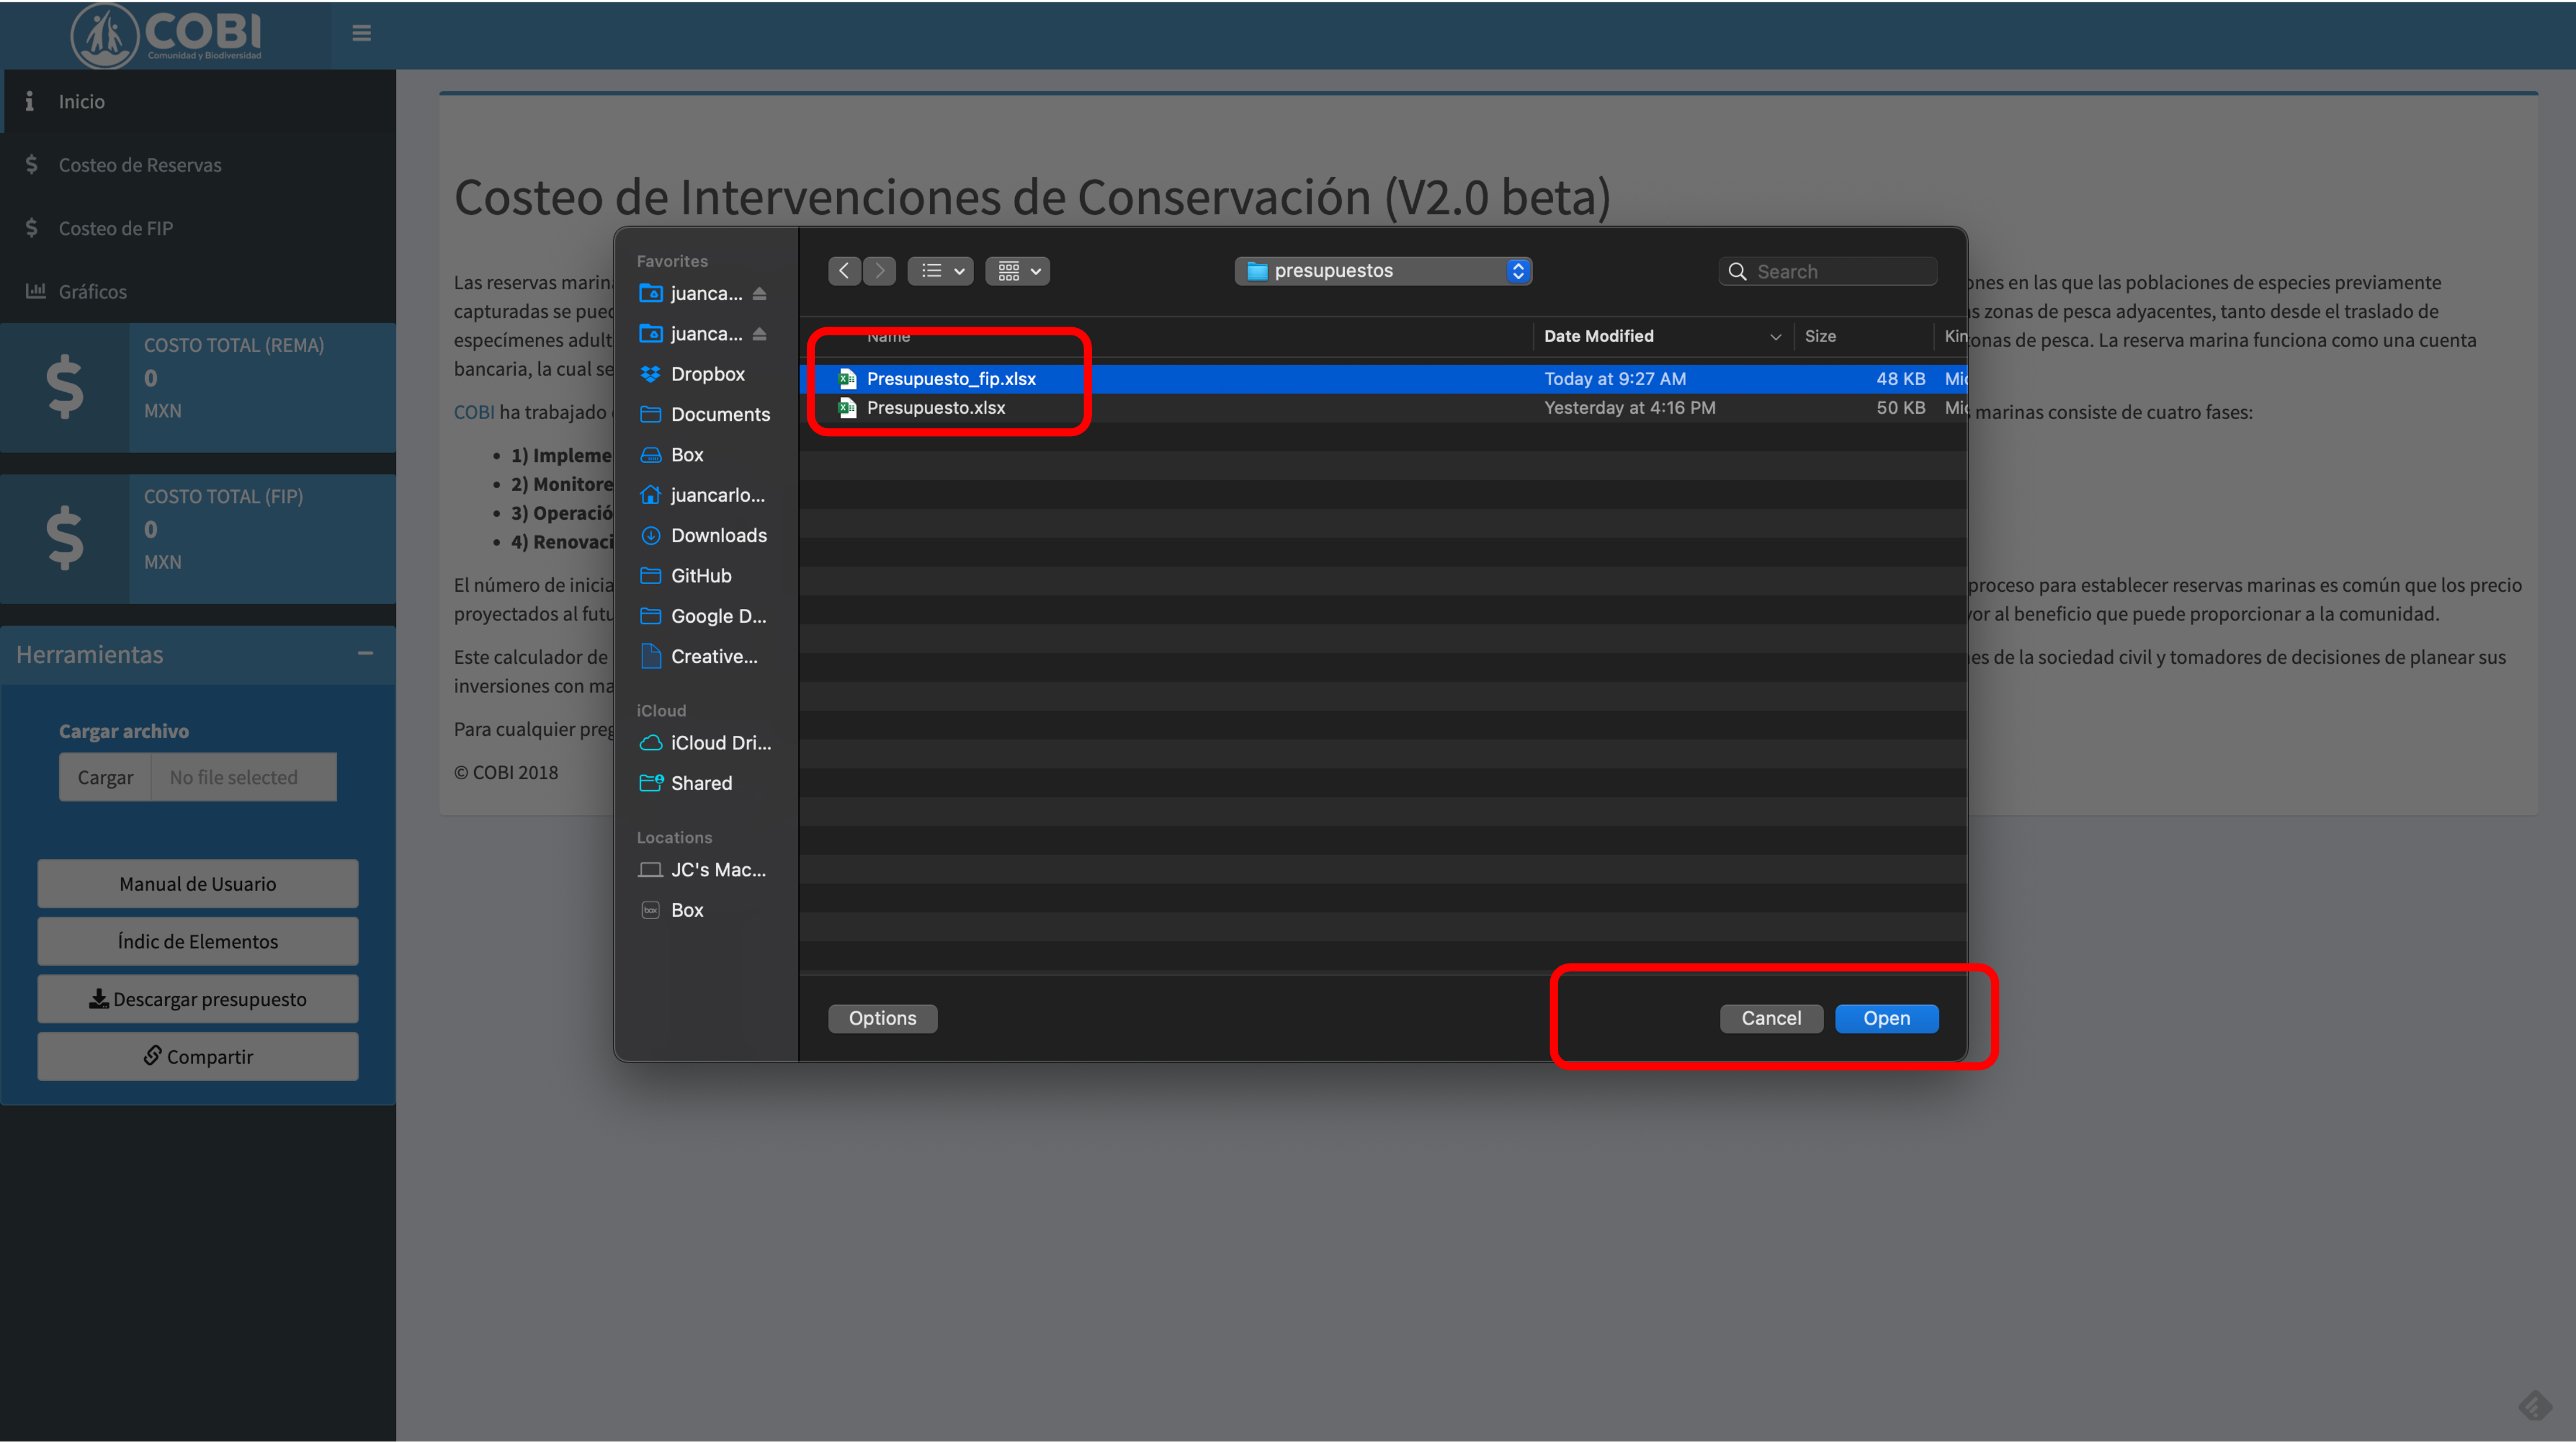
\includegraphics{images/up-2.png}
\caption{\label{fig:up-2}Asignar presupuesto a actores.}
\end{figure}

\textbf{Paso 3 - } Confirma ue el archivo fue cargado en el panel lateral \ref{fig:up-3}).

\begin{figure}
\centering
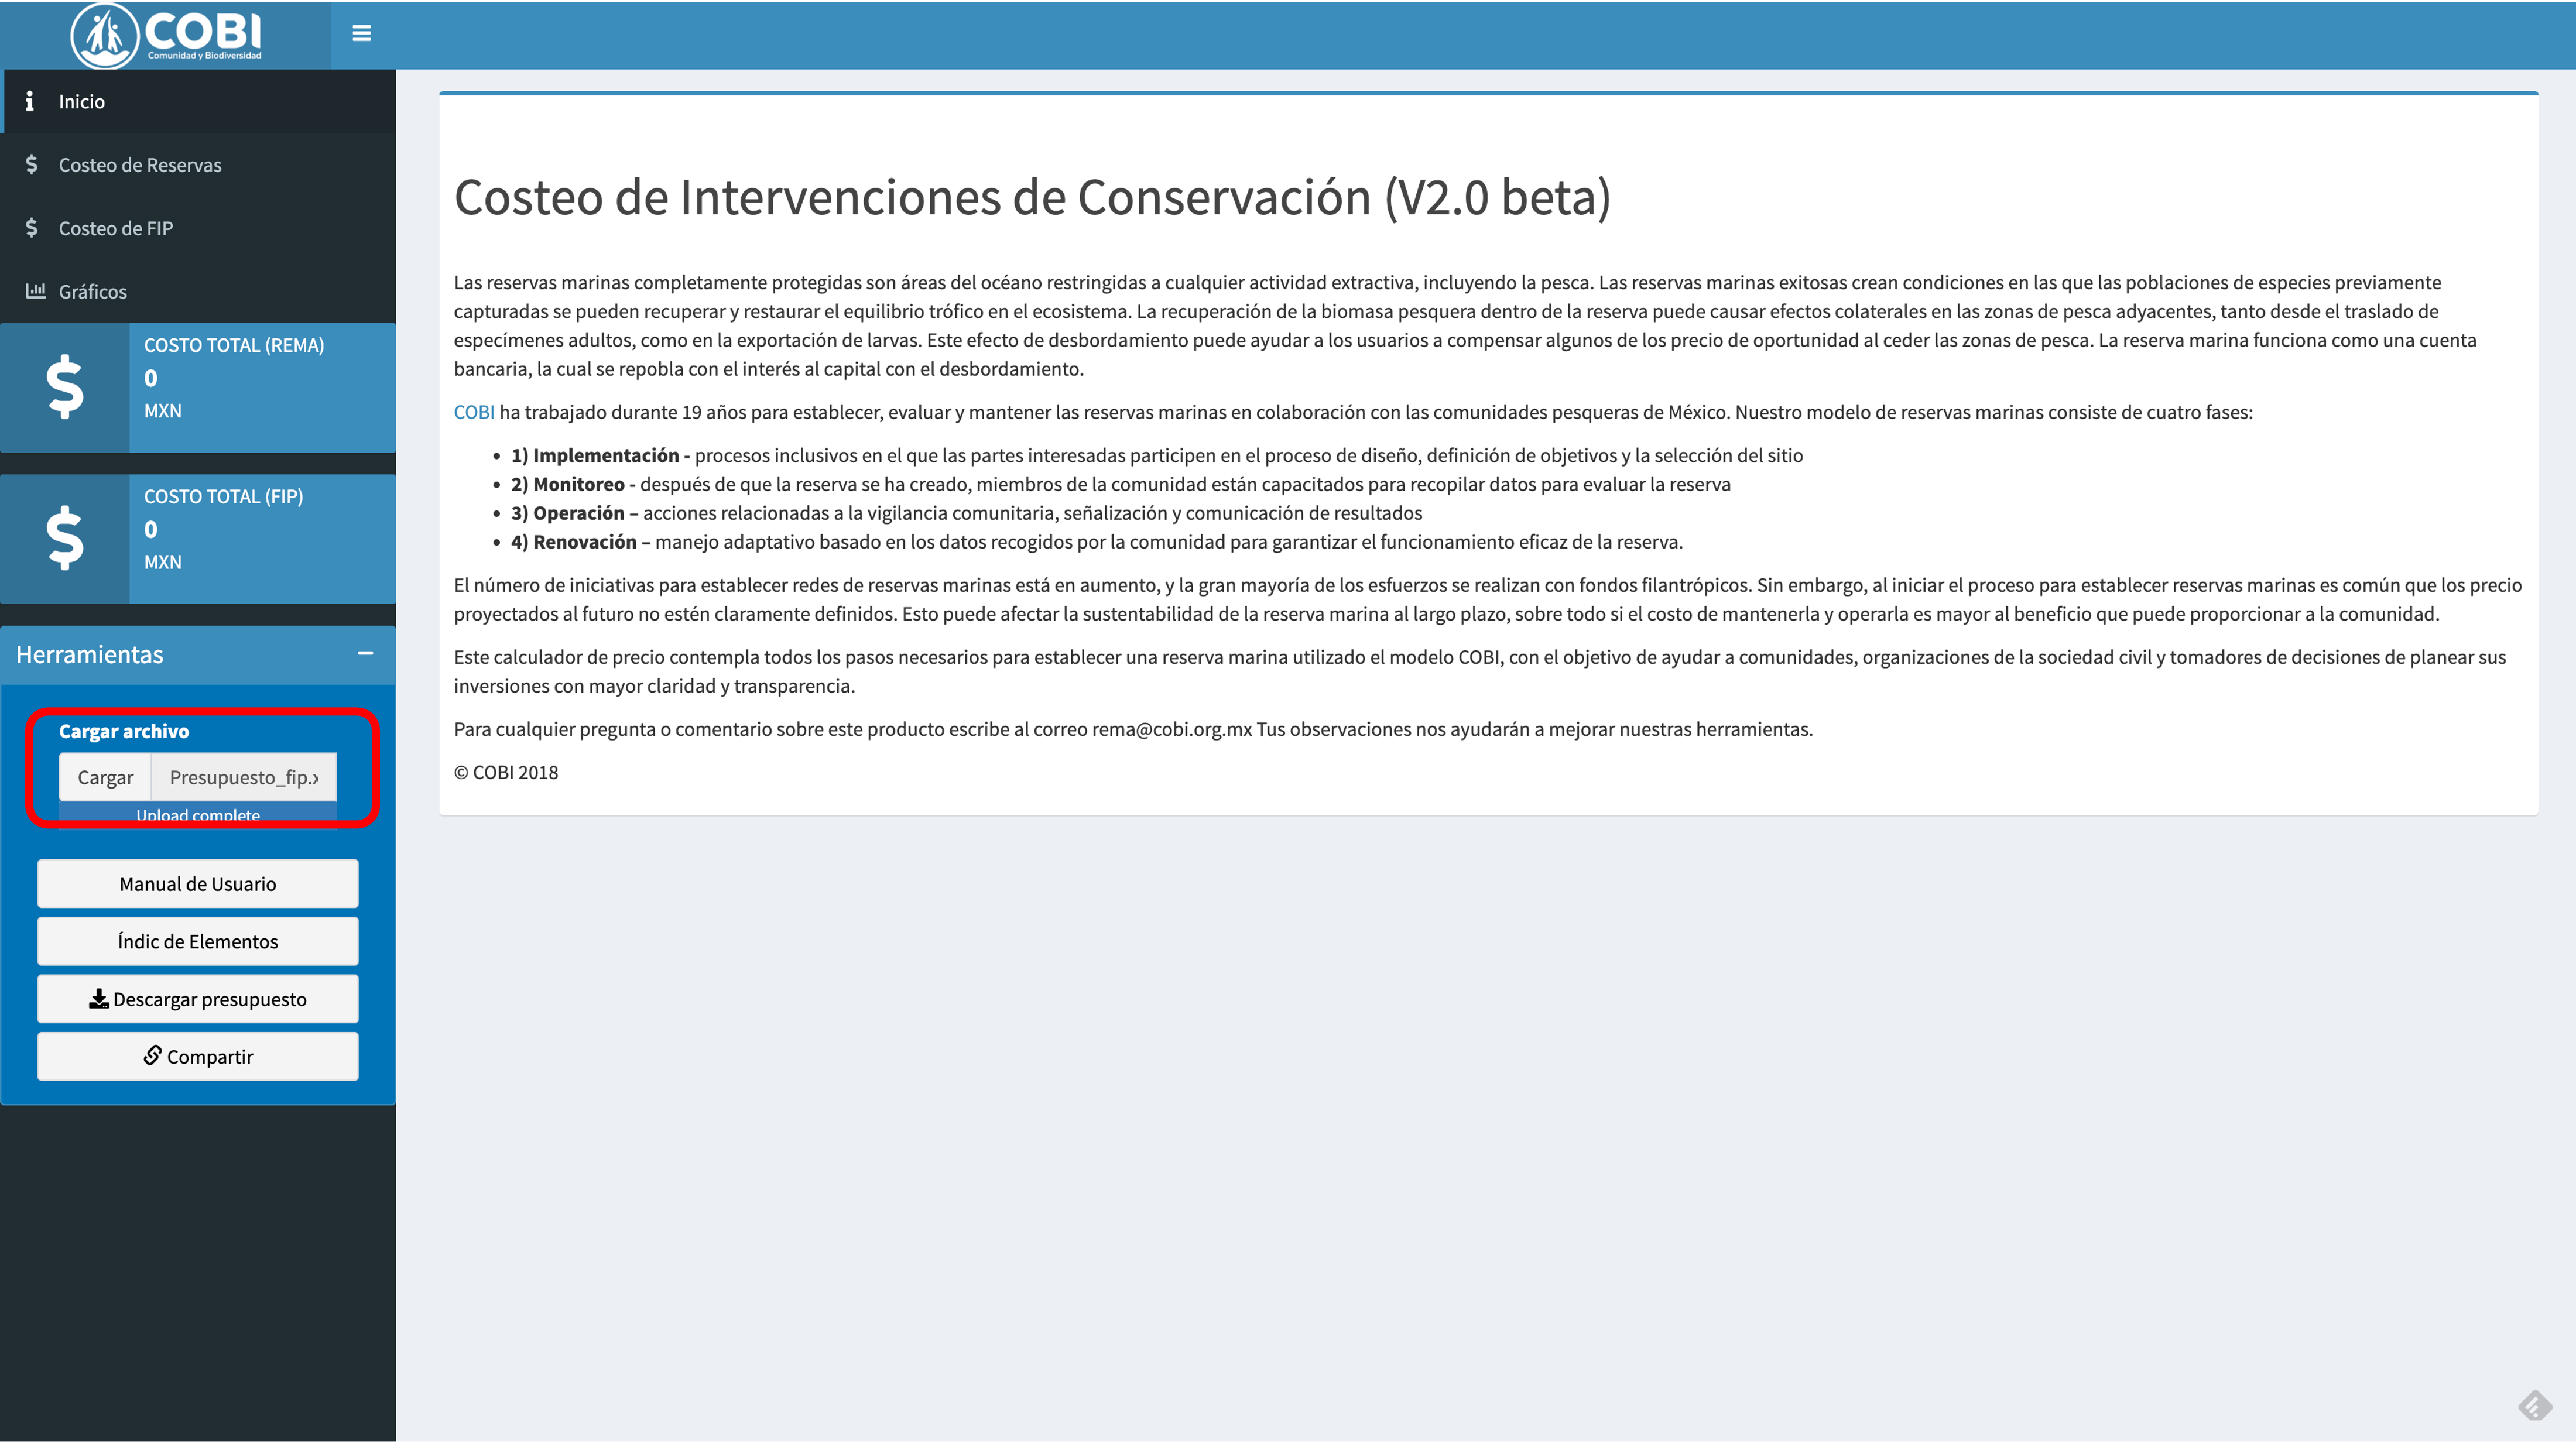
\includegraphics{images/up-3.png}
\caption{\label{fig:up-3}Asignar presupuesto a actores.}
\end{figure}

\textbf{Paso 4 - } Navega a la sección de FIP, fase de implementaión y selecciona las intervenciones correspondientes \ref{fig:up-4}). Los elementos se poblarán automáticamente con los valores que cargaste. Ahora puedes continuar editando tu progreso. Cuando hayas terminado o necesites un descanso, simplemente descarga la versión actualizada de tu presupuesto como lo vimos en el capítulo anterior.

\begin{figure}
\centering
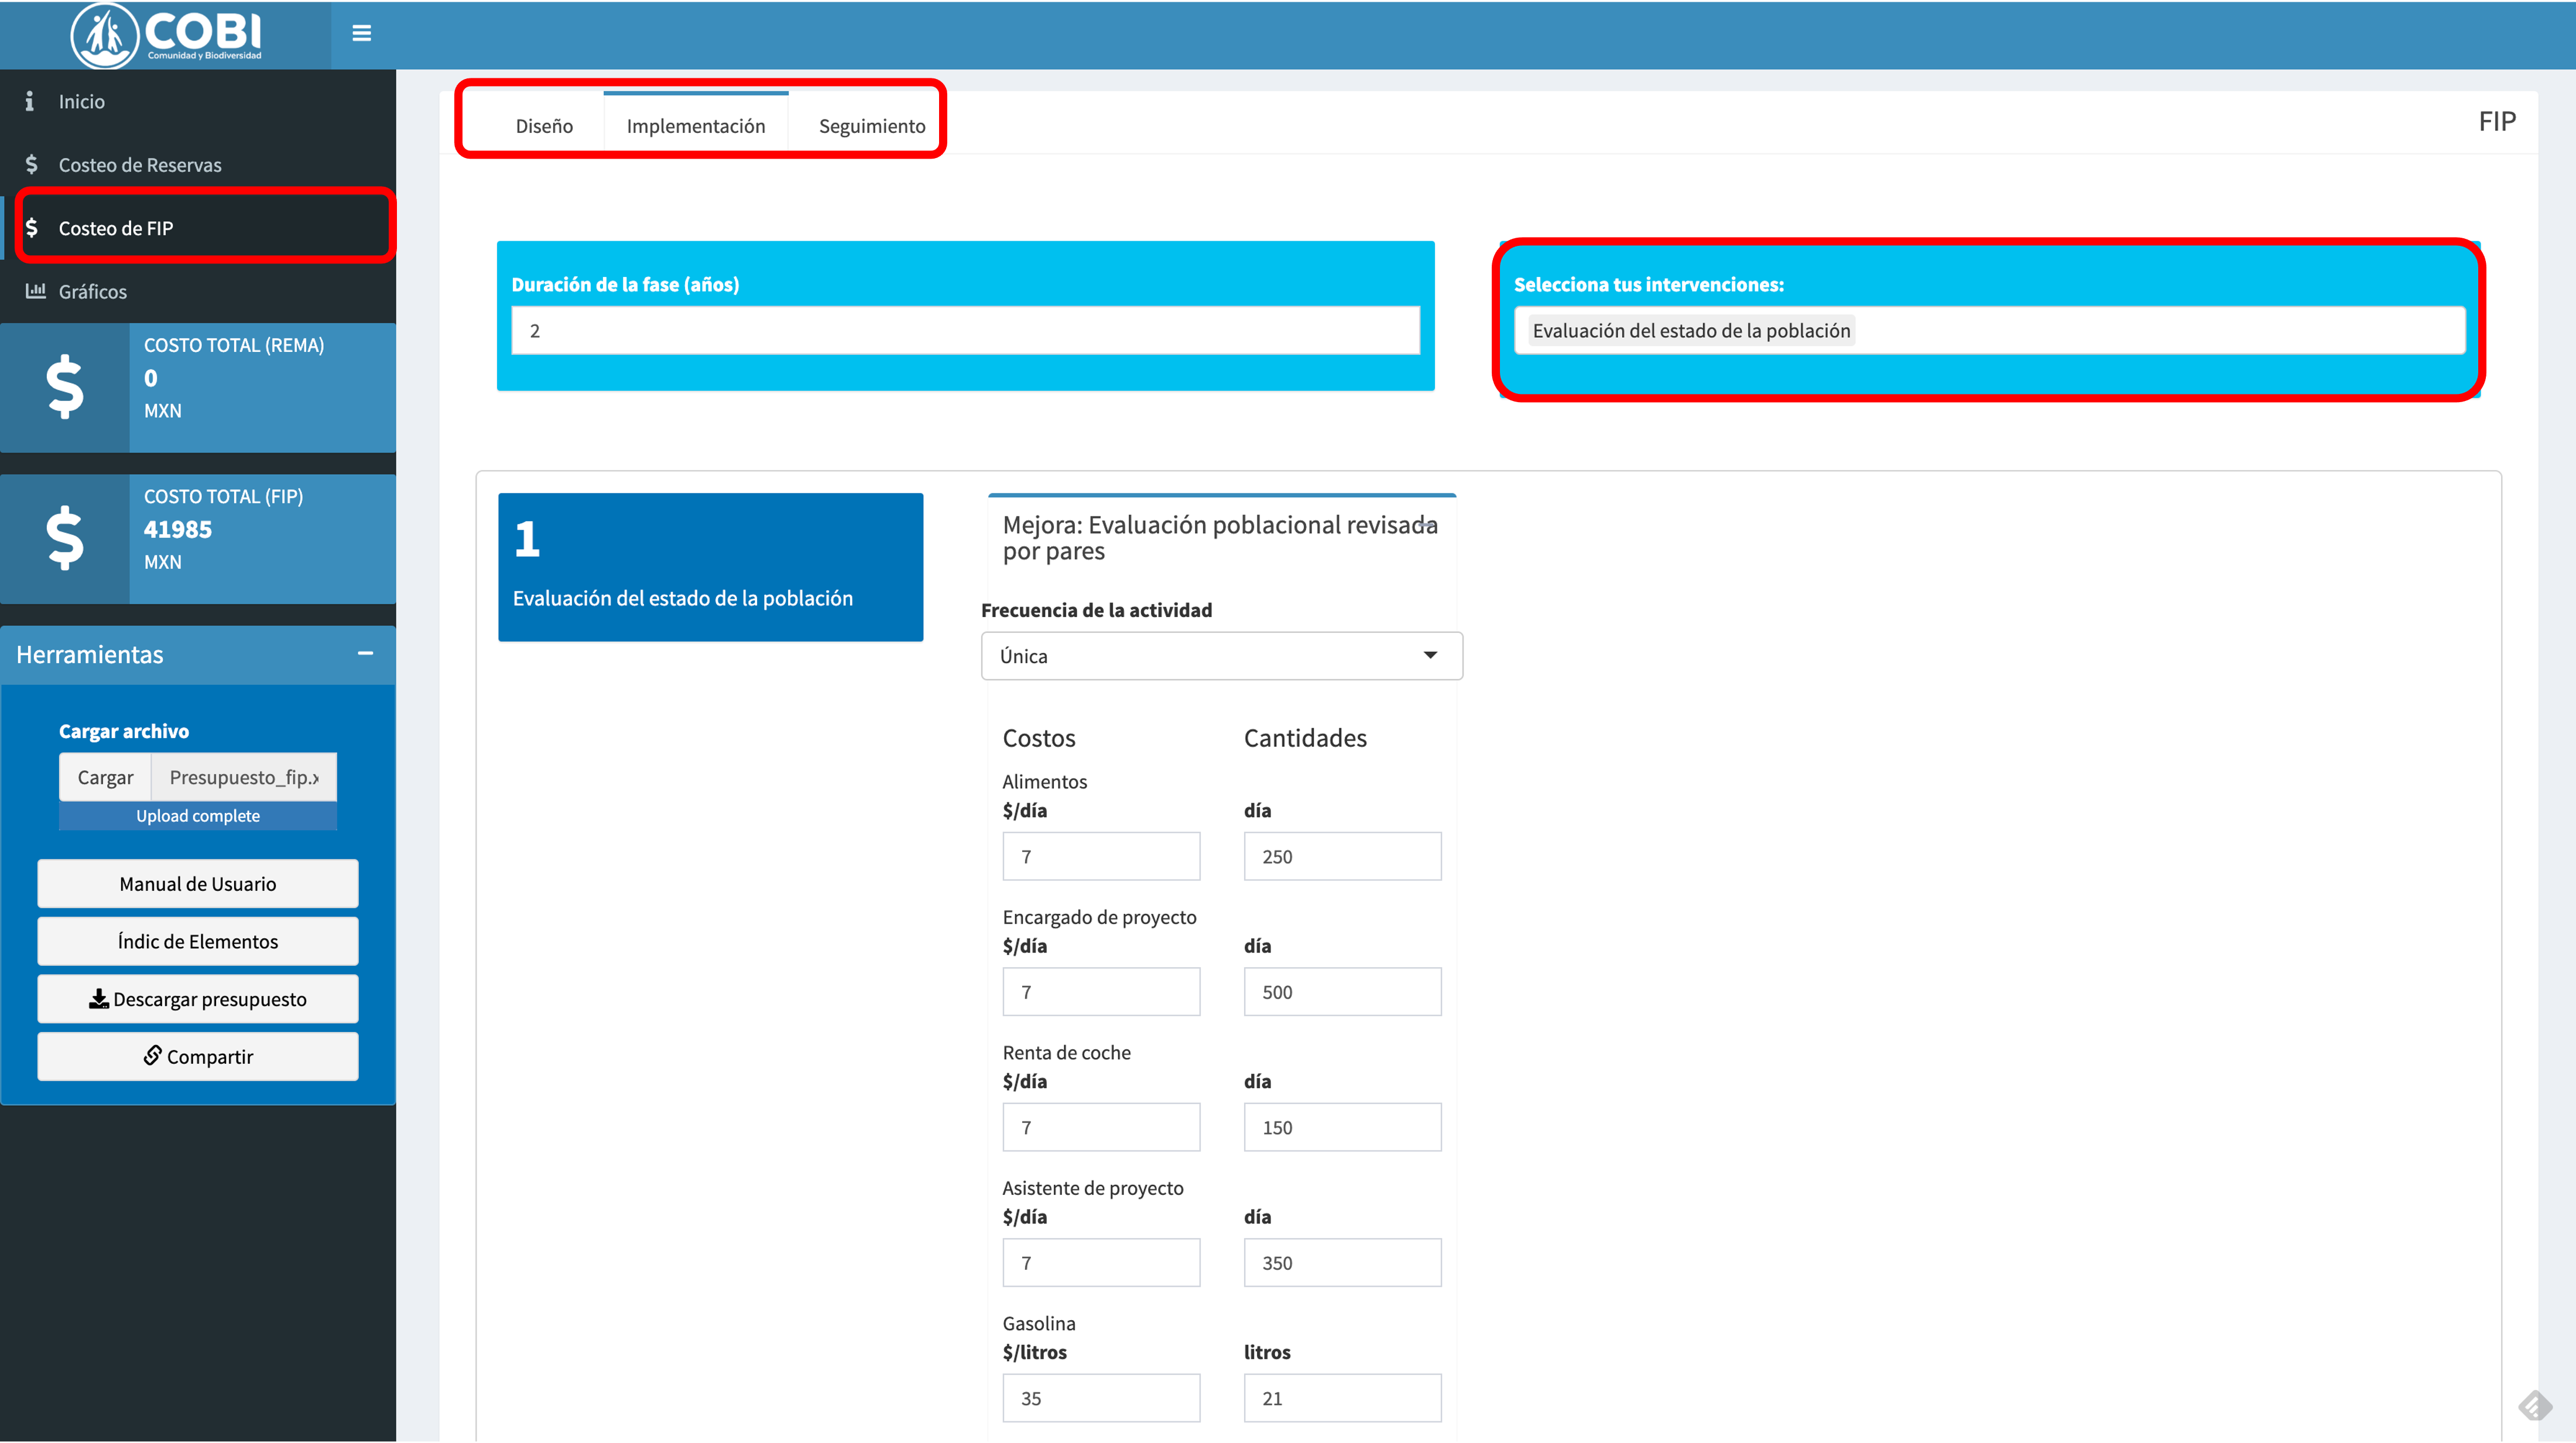
\includegraphics{images/up-4.png}
\caption{\label{fig:up-4}Asignar presupuesto a actores.}
\end{figure}

  \bibliography{book.bib,packages.bib}

\end{document}
